\documentclass[12pt,letterpaper,oneside]{book}

\usepackage[T1]{fontenc}
\usepackage[utf8]{inputenc}
\usepackage{lmodern}
\usepackage[margin=1.15in]{geometry}
\usepackage{amsmath,amssymb,amsthm}
\usepackage{booktabs}
\usepackage{multirow}
\usepackage{graphicx}
\usepackage{microtype}
\usepackage{siunitx}
\usepackage{hyperref}
\usepackage{cleveref}
\usepackage{natbib}
\usepackage{caption}
\usepackage{subcaption}
\usepackage{xcolor}
\usepackage{listings}

\hypersetup{
  colorlinks=true,
  linkcolor=black,
  citecolor=blue!50!black,
  urlcolor=blue!50!black,
  pdftitle={Constrained Selection and the Limits of the Decider Claim},
  pdfauthor={Arpit Uppal}
}

\graphicspath{{figures/}}

\newcommand{\bits}{\,\mathrm{bits/byte}}
\newcommand{\DN}{D/N}

% Every figure in the prose comes from thesis/tables/macros.tex, generated from
% result files by thesis/gen_tables.py. Nothing here is typed in by hand.
% generated by thesis/gen_tables.py — do not edit by hand
\newcommand{\CorpusTokens}{1{,}633{,}580{,}647}
\newcommand{\CorpusGB}{3.27}
\newcommand{\CorpusSha}{\texttt{9267a2ea071a5178\ldots}}
\newcommand{\CorpusDocs}{339{,}841}
\newcommand{\HoldoutPct}{2.03}
\newcommand{\HoldoutTokens}{33{,}232{,}664}
\newcommand{\TrainTokens}{1{,}600{,}347{,}983}
\newcommand{\FourBDN}{0.41}
\newcommand{\FourBTokensB}{80.0}
\newcommand{\FourBGPUHours}{22{,}222}
\newcommand{\LargeDN}{14.4}
\newcommand{\FourBFactor}{35.3}
\newcommand{\ProtoOldSpread}{0.3520}
\newcommand{\ProtoPositions}{78{,}611}
\newcommand{\ProtoNewSpread}{\emph{pending}}
\newcommand{\ProtoRatio}{\emph{pending}}
\newcommand{\LargeHeldout}{\emph{pending}}
\newcommand{\LargeTrainBits}{\emph{pending}}
\newcommand{\LargeGap}{\emph{pending}}

% generated by thesis/gen_comparator.py — do not edit by hand
\newcommand{\CmpSeeds}{11}
\newcommand{\CmpTasks}{2}
\newcommand{\CmpScoreAcc}{0.6721}
\newcommand{\CmpDecodeAcc}{0.0722}
\newcommand{\CmpDecodeInvalid}{0.790}
\newcommand{\CmpLatScore}{21.7}
\newcommand{\CmpLatDecode}{158.5}
\newcommand{\CmpLatRatio}{7.3}
\newcommand{\CmpParams}{2{,}448{,}065}
\newcommand{\CmpMB}{9.8}
\newcommand{\BreakEvenRate}{6.3}
\newcommand{\BreakEvenHigh}{11.2}
\newcommand{\CdnSlope}{84.0}
\newcommand{\CdnRTwo}{1.0000}
\newcommand{\CdnPassageTokens}{84}
\newcommand{\CdnLatCold}{21.2}
\newcommand{\CdnLatWarm}{0.52}
\newcommand{\CdnLatSpeedup}{41}
\newcommand{\CdnBillTokens}{406}
\newcommand{\CdnVerdict}{per occurrence}
\newcommand{\CmpNewsSeeds}{3}
\newcommand{\CmpNewsK}{4}
\newcommand{\CmpNewsScore}{0.5011}
\newcommand{\CmpNewsScorePct}{50.1}
\newcommand{\CmpNewsDecode}{0.1444}
\newcommand{\CmpNewsDecodePct}{14.4}
\newcommand{\CmpNewsInvalid}{0.581}
\newcommand{\CmpNewsLatScore}{15.1}
\newcommand{\CmpNewsLatDecode}{68.6}
\newcommand{\CmpNewsGpuSec}{15.1}
\newcommand{\CmpNewsRows}{300}
\newcommand{\CmpNewsScoreLo}{0.444}
\newcommand{\CmpNewsScoreHi}{0.556}
\newcommand{\CmpNewsJevTokens}{360}
\newcommand{\CmpNewsJevCost}{0.0151}
\newcommand{\CmpNewsBreakEven}{3.6}
\newcommand{\CmpBankSeeds}{3}
\newcommand{\CmpBankK}{77}
\newcommand{\CmpBankScore}{0.8430}
\newcommand{\CmpBankScorePct}{84.3}
\newcommand{\CmpBankDecode}{0.0000}
\newcommand{\CmpBankDecodePct}{0.0}
\newcommand{\CmpBankInvalid}{0.998}
\newcommand{\CmpBankLatScore}{28.2}
\newcommand{\CmpBankLatDecode}{248.4}
\newcommand{\CmpBankGpuSec}{28.2}
\newcommand{\CmpBankRows}{3000}
\newcommand{\CmpBankScoreLo}{0.830}
\newcommand{\CmpBankScoreHi}{0.856}
\newcommand{\CmpBankGap}{-5.5}
\newcommand{\CmpBankVerdict}{overlaps the cited interval; no win demonstrated}
\newcommand{\CmpBankJevTokens}{952}
\newcommand{\CmpBankJevCost}{0.0400}
\newcommand{\CmpBankBreakEven}{5.1}

% generated by thesis/gen_scaling.py — do not edit by hand
\newcommand{\RowTinyBaseAcc}{72.3}
\newcommand{\RowTinyBaseLo}{70.7}
\newcommand{\RowTinyBaseHi}{73.9}
\newcommand{\RowTinyBaseSeeds}{3}
\newcommand{\RowTinyBaseRows}{3000}
\newcommand{\RowTinyBaseLat}{24.9}
\newcommand{\RowTinyWideAcc}{84.3}
\newcommand{\RowTinyWideLo}{83.0}
\newcommand{\RowTinyWideHi}{85.6}
\newcommand{\RowTinyWideSeeds}{3}
\newcommand{\RowTinyWideRows}{3000}
\newcommand{\RowTinyWideLat}{27.4}
\newcommand{\RowSmallBaseAcc}{70.9}
\newcommand{\RowSmallBaseLo}{69.2}
\newcommand{\RowSmallBaseHi}{72.5}
\newcommand{\RowSmallBaseSeeds}{3}
\newcommand{\RowSmallBaseRows}{3000}
\newcommand{\RowSmallBaseLat}{121.7}
\newcommand{\RowSmallWideAcc}{\emph{pending}}
\newcommand{\RowSmallWideLo}{\emph{pending}}
\newcommand{\RowSmallWideHi}{\emph{pending}}
\newcommand{\RowSmallWideSeeds}{\emph{pending}}
\newcommand{\RowSmallWideRows}{\emph{pending}}
\newcommand{\RowSmallWideLat}{\emph{pending}}
\newcommand{\ShipRung}{tiny}
\newcommand{\ShipRows}{8000}
\newcommand{\ShipAcc}{84.3}
\newcommand{\ShipLo}{83.0}
\newcommand{\ShipHi}{85.6}
\newcommand{\ShipParams}{2{,}448{,}065}
\newcommand{\ShipMB}{9.8}
\newcommand{\ShipP}{27.4}
\newcommand{\ShipTestN}{1000}
\newcommand{\ShipGpuSec}{27.4}
\newcommand{\ShipBreakEven}{5.3}
\newcommand{\ShipVerdict}{overlaps the cited interval; no win demonstrated}
\newcommand{\ShipGap}{5.5}
\newcommand{\ShipSignedGap}{+5.5}
\newcommand{\ShipGapSentence}{It sits 5.5 points above the cited point estimate, but the intervals overlap, so this is not a demonstrated win; the cross-harness caveat below governs what it can be called}
\newcommand{\ShipAtJev}{yes}
\newcommand{\ShipHeadline}{Azurite is above the cited Jev point estimate but its interval overlaps the cited one: 84.3\% (95\% Wilson 83.0--85.6) against 78.8\% (73.1--83.6); this is not a demonstrated win}
\newcommand{\ShipFuture}{The remaining work is a paired harness on the same rows, which this comparison cannot provide}
\newcommand{\ShipAtNinety}{89.7}
\newcommand{\ShipAtFifty}{98.4}
\newcommand{\RowTinyGain}{+12.0}
\newcommand{\RowSmallGain}{\emph{pending}}
\newcommand{\RowRungGain}{-1.5}
\newcommand{\RowRungBase}{70.9}
\newcommand{\RowRungTiny}{72.3}
\newcommand{\RowRungGainWide}{\emph{pending}}

% generated by thesis/gen_tables.py — do not edit by hand
\newcommand{\TransferBankGain}{+42.1}
\newcommand{\TransferAgGain}{+1.13}
\newcommand{\TransferAgLo}{-2.60}
\newcommand{\TransferAgHi}{+4.80}
\newcommand{\TransferAgVerdict}{inconclusive}

% generated by thesis/gen_suite.py from results/suite_dual/SUITE.json — do not edit by hand
\newcommand{\SuiteTasks}{9}
\newcommand{\SuiteComparatorCells}{8}
\newcommand{\SuiteSmallAtOrAbove}{4}
\newcommand{\SuiteMidAtOrAbove}{3}
\newcommand{\SuiteSmallClear}{3}
\newcommand{\SuiteMidClear}{3}
\newcommand{\SuiteSmallTie}{1}
\newcommand{\SuiteMidTie}{1}
\newcommand{\SuiteSmallBelow}{4}
\newcommand{\SuiteMidBelow}{5}
\newcommand{\SuiteLargerWorse}{8}
\newcommand{\SuiteChangedCells}{8}
\newcommand{\SuiteSmallCrossChanged}{4}
\newcommand{\SuiteMidCrossChanged}{4}
\newcommand{\SuiteSmallAlreadyDual}{5}
\newcommand{\SuiteMidAlreadyDual}{5}
\newcommand{\SuiteSmallExactControls}{3}
\newcommand{\SuiteMidMinusSmallAg}{+0.55}
\newcommand{\SuiteSmallAg}{83.15}
\newcommand{\SuiteMidAg}{83.70}
\newcommand{\SuiteCitedAg}{91.00}
\newcommand{\SuiteSmallGapAg}{-7.85}
\newcommand{\SuiteMidGapAg}{-7.30}
\newcommand{\SuiteSmallPriorAg}{76.70}
\newcommand{\SuiteMidPriorAg}{80.45}
\newcommand{\SuiteSmallDeltaAg}{+6.45}
\newcommand{\SuiteMidDeltaAg}{+3.25}
\newcommand{\SuiteSmallAgLo}{81.45}
\newcommand{\SuiteSmallAgHi}{84.73}
\newcommand{\SuiteMidAgLo}{82.02}
\newcommand{\SuiteMidAgHi}{85.25}
\newcommand{\SuiteSmallEmotion}{82.25}
\newcommand{\SuiteMidEmotion}{74.15}
\newcommand{\SuiteCitedEmotion}{48.00}
\newcommand{\SuiteSmallGapEmotion}{+34.25}
\newcommand{\SuiteMidGapEmotion}{+26.15}
\newcommand{\SuiteSmallPriorEmotion}{16.45}
\newcommand{\SuiteMidPriorEmotion}{20.00}
\newcommand{\SuiteSmallDeltaEmotion}{+65.80}
\newcommand{\SuiteMidDeltaEmotion}{+54.15}
\newcommand{\SuiteSmallEmotionLo}{80.51}
\newcommand{\SuiteSmallEmotionHi}{83.86}
\newcommand{\SuiteMidEmotionLo}{72.19}
\newcommand{\SuiteMidEmotionHi}{76.02}
\newcommand{\SuiteSmallBank}{88.05}
\newcommand{\SuiteMidBank}{86.50}
\newcommand{\SuiteCitedBank}{78.80}
\newcommand{\SuiteSmallGapBank}{+9.25}
\newcommand{\SuiteMidGapBank}{+7.70}
\newcommand{\SuiteSmallPriorBank}{88.05}
\newcommand{\SuiteMidPriorBank}{82.65}
\newcommand{\SuiteSmallDeltaBank}{+0.00}
\newcommand{\SuiteMidDeltaBank}{+3.85}
\newcommand{\SuiteSmallBankLo}{86.55}
\newcommand{\SuiteSmallBankHi}{89.40}
\newcommand{\SuiteMidBankLo}{84.93}
\newcommand{\SuiteMidBankHi}{87.93}
\newcommand{\SuiteSmallClinc}{86.80}
\newcommand{\SuiteMidClinc}{82.75}
\newcommand{\SuiteCitedClinc}{89.50}
\newcommand{\SuiteSmallGapClinc}{-2.70}
\newcommand{\SuiteMidGapClinc}{-6.75}
\newcommand{\SuiteSmallPriorClinc}{86.80}
\newcommand{\SuiteMidPriorClinc}{81.80}
\newcommand{\SuiteSmallDeltaClinc}{+0.00}
\newcommand{\SuiteMidDeltaClinc}{+0.95}
\newcommand{\SuiteSmallClincLo}{85.25}
\newcommand{\SuiteSmallClincHi}{88.21}
\newcommand{\SuiteMidClincLo}{81.03}
\newcommand{\SuiteMidClincHi}{84.34}
\newcommand{\SuiteSmallMassiveIntent}{79.20}
\newcommand{\SuiteMidMassiveIntent}{77.15}
\newcommand{\SuiteCitedMassiveIntent}{78.30}
\newcommand{\SuiteSmallGapMassiveIntent}{+0.90}
\newcommand{\SuiteMidGapMassiveIntent}{-1.15}
\newcommand{\SuiteSmallPriorMassiveIntent}{79.20}
\newcommand{\SuiteMidPriorMassiveIntent}{76.35}
\newcommand{\SuiteSmallDeltaMassiveIntent}{+0.00}
\newcommand{\SuiteMidDeltaMassiveIntent}{+0.80}
\newcommand{\SuiteSmallMassiveIntentLo}{77.37}
\newcommand{\SuiteSmallMassiveIntentHi}{80.92}
\newcommand{\SuiteMidMassiveIntentLo}{75.26}
\newcommand{\SuiteMidMassiveIntentHi}{78.94}
\newcommand{\SuiteSmallMassiveScenario}{84.15}
\newcommand{\SuiteMidMassiveScenario}{80.05}
\newcommand{\SuiteCitedMassiveScenario}{---}
\newcommand{\SuiteSmallGapMassiveScenario}{---}
\newcommand{\SuiteMidGapMassiveScenario}{---}
\newcommand{\SuiteSmallPriorMassiveScenario}{84.00}
\newcommand{\SuiteMidPriorMassiveScenario}{80.70}
\newcommand{\SuiteSmallDeltaMassiveScenario}{+0.15}
\newcommand{\SuiteMidDeltaMassiveScenario}{-0.65}
\newcommand{\SuiteSmallMassiveScenarioLo}{82.48}
\newcommand{\SuiteSmallMassiveScenarioHi}{85.68}
\newcommand{\SuiteMidMassiveScenarioLo}{78.24}
\newcommand{\SuiteMidMassiveScenarioHi}{81.74}
\newcommand{\SuiteSmallXnli}{43.85}
\newcommand{\SuiteMidXnli}{35.00}
\newcommand{\SuiteCitedXnli}{86.00}
\newcommand{\SuiteSmallGapXnli}{-42.15}
\newcommand{\SuiteMidGapXnli}{-51.00}
\newcommand{\SuiteSmallPriorXnli}{32.20}
\newcommand{\SuiteMidPriorXnli}{34.40}
\newcommand{\SuiteSmallDeltaXnli}{+11.65}
\newcommand{\SuiteMidDeltaXnli}{+0.60}
\newcommand{\SuiteSmallXnliLo}{41.69}
\newcommand{\SuiteSmallXnliHi}{46.03}
\newcommand{\SuiteMidXnliLo}{32.94}
\newcommand{\SuiteMidXnliHi}{37.12}
\newcommand{\SuiteSmallLang}{96.30}
\newcommand{\SuiteMidLang}{95.60}
\newcommand{\SuiteCitedLang}{99.60}
\newcommand{\SuiteSmallGapLang}{-3.30}
\newcommand{\SuiteMidGapLang}{-4.00}
\newcommand{\SuiteSmallPriorLang}{95.15}
\newcommand{\SuiteMidPriorLang}{93.85}
\newcommand{\SuiteSmallDeltaLang}{+1.15}
\newcommand{\SuiteMidDeltaLang}{+1.75}
\newcommand{\SuiteSmallLangLo}{95.38}
\newcommand{\SuiteSmallLangHi}{97.04}
\newcommand{\SuiteMidLangLo}{94.61}
\newcommand{\SuiteMidLangHi}{96.41}
\newcommand{\SuiteSmallFinancial}{88.10}
\newcommand{\SuiteMidFinancial}{86.90}
\newcommand{\SuiteCitedFinancial}{73.00}
\newcommand{\SuiteSmallGapFinancial}{+15.10}
\newcommand{\SuiteMidGapFinancial}{+13.90}
\newcommand{\SuiteSmallPriorFinancial}{85.90}
\newcommand{\SuiteMidPriorFinancial}{85.70}
\newcommand{\SuiteSmallDeltaFinancial}{+2.20}
\newcommand{\SuiteMidDeltaFinancial}{+1.20}
\newcommand{\SuiteSmallFinancialLo}{85.95}
\newcommand{\SuiteSmallFinancialHi}{89.96}
\newcommand{\SuiteMidFinancialLo}{84.67}
\newcommand{\SuiteMidFinancialHi}{88.85}
\newcommand{\SuiteEmotionMajority}{34.75}
\newcommand{\SuiteEmotionUniform}{16.67}
\newcommand{\SuiteSmallEmotionNll}{1.2542}
\newcommand{\SuiteMidEmotionNll}{1.9037}
\newcommand{\SuiteSmallEmotionEce}{0.1366}
\newcommand{\SuiteMidEmotionEce}{0.2183}
\newcommand{\SuiteEmotionRungDrop}{8.10}
\newcommand{\SuiteSmallXnliRaw}{32.20}
\newcommand{\SuiteMidXnliRaw}{34.40}
\newcommand{\SuiteSmallXnliGain}{+11.65}
\newcommand{\SuiteMidXnliGain}{+0.60}
\newcommand{\SuiteSmallXnliShortfall}{42.15}
\newcommand{\SuiteMidXnliShortfall}{51.00}
\newcommand{\SuiteXnliChance}{33.33}
\newcommand{\SuiteSmallXnliPriorFix}{39.50}
\newcommand{\SuiteXnliAbsentTest}{699}
\newcommand{\SuiteXnliAbsentTrain}{1473}
\newcommand{\SuiteXnliFullFixed}{1828}
\newcommand{\SuiteXnliTestN}{2000}
\newcommand{\SuiteXnliTrainN}{4000}

% generated by thesis/gen_suite_three.py from results/suite_large_113m — do not edit by hand
\newcommand{\SuiteLargeAtOrAbove}{5}
\newcommand{\SuiteLargeClear}{4}
\newcommand{\SuiteLargeTie}{1}
\newcommand{\SuiteLargeBelow}{3}
\newcommand{\SuiteSmallAtOrAboveThree}{4}
\newcommand{\SuiteMidAtOrAboveThree}{4}
\newcommand{\SuiteRungs}{3}
\newcommand{\SuiteTotalCells}{27}
\newcommand{\SuiteLargeWins}{4}
\newcommand{\SuiteLargeLosses}{1}
\newcommand{\SuiteLargeUnmoved}{4}
\newcommand{\SuiteLargeWinMin}{+1.70}
\newcommand{\SuiteLargeWinMax}{+2.80}
\newcommand{\SuiteLargeLossMin}{-9.95}
\newcommand{\SuiteLargeLossMax}{-9.95}
\newcommand{\SuiteLargeLossAbs}{9.95}
\newcommand{\SuiteLargeWinCells}{AG News, CLINC150, MASSIVE intent and Financial PhraseBank}
\newcommand{\SuiteLargeLossOverWinMax}{3.6}
\newcommand{\SuiteLargeAg}{85.75}
\newcommand{\SuiteLargeGapAg}{-5.25}
\newcommand{\SuiteLargeShortAg}{5.25}
\newcommand{\SuiteLargeAgLo}{84.15}
\newcommand{\SuiteLargeAgHi}{87.21}
\newcommand{\SuiteLargeOnlyAg}{146}
\newcommand{\SuiteSmallOnlyAg}{94}
\newcommand{\SuiteLargeVSSmallPAg}{9.55e-04}
\newcommand{\SuiteLargeVsSmallAg}{+2.60}
\newcommand{\SuiteLargeEmotion}{81.70}
\newcommand{\SuiteLargeGapEmotion}{+33.70}
\newcommand{\SuiteLargeShortEmotion}{33.70}
\newcommand{\SuiteLargeEmotionLo}{79.95}
\newcommand{\SuiteLargeEmotionHi}{83.33}
\newcommand{\SuiteLargeOnlyEmotion}{162}
\newcommand{\SuiteSmallOnlyEmotion}{173}
\newcommand{\SuiteLargeVSSmallPEmotion}{5.85e-01}
\newcommand{\SuiteLargeVsSmallEmotion}{-0.55}
\newcommand{\SuiteLargeBank}{88.45}
\newcommand{\SuiteLargeGapBank}{+9.65}
\newcommand{\SuiteLargeShortBank}{9.65}
\newcommand{\SuiteLargeBankLo}{86.97}
\newcommand{\SuiteLargeBankHi}{89.78}
\newcommand{\SuiteLargeOnlyBank}{84}
\newcommand{\SuiteSmallOnlyBank}{76}
\newcommand{\SuiteLargeVSSmallPBank}{5.80e-01}
\newcommand{\SuiteLargeVsSmallBank}{+0.40}
\newcommand{\SuiteLargeClinc}{88.50}
\newcommand{\SuiteLargeGapClinc}{-1.00}
\newcommand{\SuiteLargeShortClinc}{1.00}
\newcommand{\SuiteLargeClincLo}{87.03}
\newcommand{\SuiteLargeClincHi}{89.82}
\newcommand{\SuiteLargeOnlyClinc}{102}
\newcommand{\SuiteSmallOnlyClinc}{68}
\newcommand{\SuiteLargeVSSmallPClinc}{1.12e-02}
\newcommand{\SuiteLargeVsSmallClinc}{+1.70}
\newcommand{\SuiteLargeMassiveIntent}{82.00}
\newcommand{\SuiteLargeGapMassiveIntent}{+3.70}
\newcommand{\SuiteLargeShortMassiveIntent}{3.70}
\newcommand{\SuiteLargeMassiveIntentLo}{80.26}
\newcommand{\SuiteLargeMassiveIntentHi}{83.62}
\newcommand{\SuiteLargeOnlyMassiveIntent}{127}
\newcommand{\SuiteSmallOnlyMassiveIntent}{71}
\newcommand{\SuiteLargeVSSmallPMassiveIntent}{8.39e-05}
\newcommand{\SuiteLargeVsSmallMassiveIntent}{+2.80}
\newcommand{\SuiteLargeMassiveScenario}{83.90}
\newcommand{\SuiteLargeGapMassiveScenario}{---}
\newcommand{\SuiteLargeMassiveScenarioLo}{82.22}
\newcommand{\SuiteLargeMassiveScenarioHi}{85.45}
\newcommand{\SuiteLargeOnlyMassiveScenario}{83}
\newcommand{\SuiteSmallOnlyMassiveScenario}{88}
\newcommand{\SuiteLargeVSSmallPMassiveScenario}{7.60e-01}
\newcommand{\SuiteLargeVsSmallMassiveScenario}{-0.25}
\newcommand{\SuiteLargeXnli}{33.90}
\newcommand{\SuiteLargeGapXnli}{-52.10}
\newcommand{\SuiteLargeShortXnli}{52.10}
\newcommand{\SuiteLargeXnliLo}{31.86}
\newcommand{\SuiteLargeXnliHi}{36.00}
\newcommand{\SuiteLargeOnlyXnli}{402}
\newcommand{\SuiteSmallOnlyXnli}{601}
\newcommand{\SuiteLargeVSSmallPXnli}{3.56e-10}
\newcommand{\SuiteLargeVsSmallXnli}{-9.95}
\newcommand{\SuiteLargeLang}{95.80}
\newcommand{\SuiteLargeGapLang}{-3.80}
\newcommand{\SuiteLargeShortLang}{3.80}
\newcommand{\SuiteLargeLangLo}{94.83}
\newcommand{\SuiteLargeLangHi}{96.59}
\newcommand{\SuiteLargeOnlyLang}{24}
\newcommand{\SuiteSmallOnlyLang}{34}
\newcommand{\SuiteLargeVSSmallPLang}{2.37e-01}
\newcommand{\SuiteLargeVsSmallLang}{-0.50}
\newcommand{\SuiteLargeFinancial}{90.10}
\newcommand{\SuiteLargeGapFinancial}{+17.10}
\newcommand{\SuiteLargeShortFinancial}{17.10}
\newcommand{\SuiteLargeFinancialLo}{88.09}
\newcommand{\SuiteLargeFinancialHi}{91.80}
\newcommand{\SuiteLargeOnlyFinancial}{56}
\newcommand{\SuiteSmallOnlyFinancial}{36}
\newcommand{\SuiteLargeVSSmallPFinancial}{4.70e-02}
\newcommand{\SuiteLargeVsSmallFinancial}{+2.00}
\newcommand{\SuiteSmallXnliNll}{2.12}
\newcommand{\SuiteSmallXnliEce}{0.36}
\newcommand{\SuiteMidXnliNll}{3.18}
\newcommand{\SuiteMidXnliEce}{0.42}
\newcommand{\SuiteLargeXnliNll}{1.0986}
\newcommand{\SuiteLargeXnliLnK}{1.0986}
\newcommand{\SuiteLargeXnliConf}{0.3337}
\newcommand{\SuiteLargeXnliEce}{0.0053}
\newcommand{\SuiteLargeXnliTopShare}{94.7}
\newcommand{\SuiteLargeXnliChance}{33.33}
\newcommand{\SuiteLargeXnliTopClass}{2}
\newcommand{\SuiteLargeXnliUniform}{yes}
\newcommand{\SuiteLostTokens}{980{,}746{,}240}
\newcommand{\SuiteLostTarget}{1{,}134{,}658{,}560}
\newcommand{\SuiteLostPct}{86.44}
\newcommand{\SuiteLostStep}{59{,}860}
\newcommand{\SuiteLostSegments}{11}
\newcommand{\SuitePreRegSha}{09db4c6b374049f4\ldots}
\newcommand{\SuiteCkptLarge}{aba65b60e30654a9\ldots}
\newcommand{\SuiteCkptLargeStep}{69{,}255}
\newcommand{\SuiteCkptLargeTokens}{1{,}134{,}673{,}920}
\newcommand{\SuiteReplicationMax}{1.25}
\newcommand{\SuiteReplicationMean}{0.68}
\newcommand{\SuiteReplicationFlips}{274}
\newcommand{\SuiteReplicationCells}{3}
\newcommand{\SuiteLargeGpuHours}{8.34}
\newcommand{\SuiteLargeParamsRatio}{7.96}

% generated by thesis/gen_e4.py from results/e4_candidate_sweep — do not edit
\newcommand{\ETasks}{3}
\newcommand{\EMaxHarnessDelta}{0.80}
\newcommand{\EHolds}{3}
\newcommand{\EAggregateVerdict}{holds}
\newcommand{\EMargin}{5.0}
\newcommand{\EPreregSha}{762739463e8b5c97\ldots}
\newcommand{\ECheckpoint}{aba65b60e30654a9\ldots}
\newcommand{\EArms}{12}
\newcommand{\EArmHours}{0.78}
\newcommand{\EFutureHours}{18.6}
\newcommand{\EFutureBothHours}{27.9}
\newcommand{\ESweepHours}{9.3}
\newcommand{\ECostMin}{8.90}
\newcommand{\ECostMax}{14.80}
\newcommand{\ECostTwoToThirtyTwoMin}{5.80}
\newcommand{\ECostTwoToThirtyTwoMax}{13.85}
\newcommand{\EBankK}{77}
\newcommand{\EBankWTwo}{98.05}
\newcommand{\EBankWTwoLo}{97.35}
\newcommand{\EBankWTwoHi}{98.57}
\newcommand{\EBankWEight}{95.95}
\newcommand{\EBankWEightLo}{94.99}
\newcommand{\EBankWEightHi}{96.73}
\newcommand{\EBankWThirtyTwo}{92.10}
\newcommand{\EBankWThirtyTwoLo}{90.84}
\newcommand{\EBankWThirtyTwoHi}{93.20}
\newcommand{\EBankWK}{89.15}
\newcommand{\EBankWKLo}{87.71}
\newcommand{\EBankWKHi}{90.44}
\newcommand{\EBankDelta}{+2.95}
\newcommand{\EBankLower}{+1.95}
\newcommand{\EBankP}{2.08e-06}
\newcommand{\EBankVerdict}{holds}
\newcommand{\EBankHarnessDelta}{0.70}
\newcommand{\EBankPublished}{88.45}
\newcommand{\EBankHarnessOK}{no}
\newcommand{\EBankWidthTwo}{+8.90}
\newcommand{\EBankWidthTwoCost}{8.90}
\newcommand{\EBankWidthEightVsThirtyTwo}{+3.85}
\newcommand{\EBankFullKAtTwo}{70.25}
\newcommand{\EBankFullKAtEight}{83.70}
\newcommand{\EBankFullKAtThirtyTwo}{87.85}
\newcommand{\EBankCostTwoToThirtyTwo}{5.95}
\newcommand{\EClincK}{151}
\newcommand{\EClincWTwo}{98.00}
\newcommand{\EClincWTwoLo}{97.29}
\newcommand{\EClincWTwoHi}{98.53}
\newcommand{\EClincWEight}{95.25}
\newcommand{\EClincWEightLo}{94.23}
\newcommand{\EClincWEightHi}{96.10}
\newcommand{\EClincWThirtyTwo}{92.20}
\newcommand{\EClincWThirtyTwoLo}{90.94}
\newcommand{\EClincWThirtyTwoHi}{93.30}
\newcommand{\EClincWK}{87.70}
\newcommand{\EClincWKLo}{86.19}
\newcommand{\EClincWKHi}{89.07}
\newcommand{\EClincDelta}{+4.50}
\newcommand{\EClincLower}{+3.45}
\newcommand{\EClincP}{2.63e-12}
\newcommand{\EClincVerdict}{holds}
\newcommand{\EClincHarnessDelta}{0.80}
\newcommand{\EClincPublished}{88.50}
\newcommand{\EClincHarnessOK}{no}
\newcommand{\EClincWidthTwo}{+10.30}
\newcommand{\EClincWidthTwoCost}{10.30}
\newcommand{\EClincWidthEightVsThirtyTwo}{+3.05}
\newcommand{\EClincFullKAtTwo}{64.80}
\newcommand{\EClincFullKAtEight}{81.55}
\newcommand{\EClincFullKAtThirtyTwo}{85.55}
\newcommand{\EClincCostTwoToThirtyTwo}{5.80}
\newcommand{\EMassiveK}{60}
\newcommand{\EMassiveWTwo}{96.70}
\newcommand{\EMassiveWTwoLo}{95.82}
\newcommand{\EMassiveWTwoHi}{97.40}
\newcommand{\EMassiveWEight}{91.40}
\newcommand{\EMassiveWEightLo}{90.09}
\newcommand{\EMassiveWEightHi}{92.55}
\newcommand{\EMassiveWThirtyTwo}{82.85}
\newcommand{\EMassiveWThirtyTwoLo}{81.14}
\newcommand{\EMassiveWThirtyTwoHi}{84.44}
\newcommand{\EMassiveWK}{81.90}
\newcommand{\EMassiveWKLo}{80.15}
\newcommand{\EMassiveWKHi}{83.53}
\newcommand{\EMassiveDelta}{+0.95}
\newcommand{\EMassiveLower}{-0.20}
\newcommand{\EMassiveP}{2.06e-01}
\newcommand{\EMassiveVerdict}{holds}
\newcommand{\EMassiveHarnessDelta}{0.10}
\newcommand{\EMassivePublished}{82.00}
\newcommand{\EMassiveHarnessOK}{yes}
\newcommand{\EMassiveWidthTwo}{+14.80}
\newcommand{\EMassiveWidthTwoCost}{14.80}
\newcommand{\EMassiveWidthEightVsThirtyTwo}{+8.55}
\newcommand{\EMassiveFullKAtTwo}{69.25}
\newcommand{\EMassiveFullKAtEight}{78.70}
\newcommand{\EMassiveFullKAtThirtyTwo}{78.55}
\newcommand{\EMassiveCostTwoToThirtyTwo}{13.85}

% generated by thesis/gen_jev_matched.py — do not edit by hand
\newcommand{\JevMatchN}{3{,}080}
\newcommand{\JevMatchCorrectJev}{2{,}846}
\newcommand{\JevMatchPctJev}{92.40}
\newcommand{\JevMatchJevLo}{91.41}
\newcommand{\JevMatchJevHi}{93.29}
\newcommand{\JevMatchCorrectNoEx}{2{,}722}
\newcommand{\JevMatchPctNoEx}{88.38}
\newcommand{\JevMatchNoExLo}{87.20}
\newcommand{\JevMatchNoExHi}{89.46}
\newcommand{\JevMatchGapNoEx}{-4.03}
\newcommand{\JevMatchLowerNoEx}{-4.97}
\newcommand{\JevMatchPNoEx}{8.49\times10^{-12}}
\newcommand{\JevMatchCorrectATwo}{1{,}793}
\newcommand{\JevMatchPctATwo}{58.21}
\newcommand{\JevMatchATwoLo}{56.46}
\newcommand{\JevMatchATwoHi}{59.94}
\newcommand{\JevMatchGapATwo}{-34.19}
\newcommand{\JevMatchLowerATwo}{-35.78}
\newcommand{\JevMatchPATwo}{1.21\times10^{-237}}
\newcommand{\JevMatchCorrectAOne}{691}
\newcommand{\JevMatchPctAOne}{22.44}
\newcommand{\JevMatchAOneLo}{21.00}
\newcommand{\JevMatchAOneHi}{23.94}
\newcommand{\JevMatchGapAOne}{-69.97}
\newcommand{\JevMatchLowerAOne}{-71.40}
\newcommand{\JevMatchPAOne}{<10^{-300}}
\newcommand{\JevMatchEffATwo}{12.2}
\newcommand{\JevMatchEffATwoMin}{2}
\newcommand{\JevMatchEffATwoMax}{20}
\newcommand{\JevMatchEffAOne}{24.0}
\newcommand{\JevMatchHeadSteps}{3{,}000}
\newcommand{\JevMatchArms}{3}
\newcommand{\JevMatchPreregSha}{ee1b5bb51a7b}
\newcommand{\JevMatchAmendmentSha}{73f3fdc46cc1}
\newcommand{\JevMatchVerdict}{the gap survives}
\newcommand{\JevMatchMargin}{2.0}
\newcommand{\JevMatchGapPrimary}{4.03}
\newcommand{\JevMatchAbsGapAOne}{69.97}
\newcommand{\JevMatchAbsGapNoEx}{4.03}
\newcommand{\JevMatchDistinctNoEx}{77}
\newcommand{\JevMatchTopNoEx}{1.6}
\newcommand{\JevMatchDistinctAOne}{64}
\newcommand{\JevMatchTopAOne}{14.3}
\newcommand{\JevMatchTopThreeAOne}{35.4}

% generated by thesis/gen_query.py — do not edit by hand
\newcommand{\QueryJevPct}{92.40}
\newcommand{\QueryN}{3{,}080}
\newcommand{\QueryEff}{11.9}
\newcommand{\QueryEffMin}{2}
\newcommand{\QueryEffMax}{19}
\newcommand{\QueryVerdict}{P0 missed}
\newcommand{\QueryPrereg}{bde97e74f2f8}
\newcommand{\QueryHeadSha}{7992c97362b3}
\newcommand{\QueryNonInferior}{no}
\newcommand{\QueryCorrectOldZero}{2{,}722}
\newcommand{\QueryPctOldZero}{88.38}
\newcommand{\QueryLoOldZero}{87.20}
\newcommand{\QueryHiOldZero}{89.46}
\newcommand{\QueryGapOldZero}{-4.03}
\newcommand{\QueryLowerOldZero}{-4.97}
\newcommand{\QueryPOldZero}{$8.49\times10^{-12}$}
\newcommand{\QueryCorrectOldTwo}{1{,}821}
\newcommand{\QueryPctOldTwo}{59.12}
\newcommand{\QueryLoOldTwo}{57.38}
\newcommand{\QueryHiOldTwo}{60.85}
\newcommand{\QueryGapOldTwo}{-33.28}
\newcommand{\QueryLowerOldTwo}{-34.87}
\newcommand{\QueryPOldTwo}{$2.96\times10^{-231}$}
\newcommand{\QueryCorrectQueryZero}{1{,}880}
\newcommand{\QueryPctQueryZero}{61.04}
\newcommand{\QueryLoQueryZero}{59.30}
\newcommand{\QueryHiQueryZero}{62.75}
\newcommand{\QueryGapQueryZero}{-31.36}
\newcommand{\QueryLowerQueryZero}{-32.82}
\newcommand{\QueryPQueryZero}{$1.82\times10^{-226}$}
\newcommand{\QueryCorrectQueryTwo}{2{,}742}
\newcommand{\QueryPctQueryTwo}{89.03}
\newcommand{\QueryLoQueryTwo}{87.87}
\newcommand{\QueryHiQueryTwo}{90.08}
\newcommand{\QueryGapQueryTwo}{-3.38}
\newcommand{\QueryLowerQueryTwo}{-4.32}
\newcommand{\QueryPQueryTwo}{$3.99\times10^{-9}$}
\newcommand{\QueryDiff}{-3.38}
\newcommand{\QueryDiffAbs}{3.38}
\newcommand{\QueryLowerPrimary}{-4.32}
\newcommand{\QueryPValue}{$3.99\times10^{-9}$}
\newcommand{\QueryPValueText}{p = 3.99\times10^{-9}}
\newcommand{\QueryMechPText}{p = 3.62\times10^{-212}}
\newcommand{\QueryMechGain}{+29.90}
\newcommand{\QueryMechGainAbs}{29.90}
\newcommand{\QueryMechLower}{+28.41}
\newcommand{\QueryMechP}{$3.62\times10^{-212}$}
\newcommand{\QueryVsZeroGain}{+27.99}
\newcommand{\QueryVsOldZeroGain}{+0.65}
\newcommand{\QueryTrainMinutes}{58}
\newcommand{\QuerySecStep}{1.16}
\newcommand{\QueryLastLoss}{0.0004}
\newcommand{\QueryNextShortHours}{5.4}
\newcommand{\QueryNextLongLo}{17.0}
\newcommand{\QueryNextLongHi}{34.1}

% generated by thesis/gen_query_5120.py — do not edit by hand
\newcommand{\LenJevPct}{92.40}
\newcommand{\LenN}{3{,}080}
\newcommand{\LenPrereg}{c59b5e08d916}
\newcommand{\LenAmendment}{7993177d769a}
\newcommand{\LenInitSha}{5294fd685615}
\newcommand{\LenHeadSha}{e7455fc462e9}
\newcommand{\LenVerdict}{P0 missed}
\newcommand{\LenPZeroMet}{0}
\newcommand{\LenEff}{24.0}
\newcommand{\LenEffMin}{24}
\newcommand{\LenEffMax}{24}
\newcommand{\LenContextMax}{4{,}714}
\newcommand{\LenNonInferior}{no}
\newcommand{\LenHeadHours}{1.69}
\newcommand{\LenTotalHours}{1.69}
\newcommand{\LenSteps}{3{,}000}
\newcommand{\LenBatch}{8}
\newcommand{\LenSecStep}{2.02}
\newcommand{\LenTrainPct}{96.62}
\newcommand{\LenTrainCorrect}{3{,}865}
\newcommand{\LenTrainLoss}{0.1321}
\newcommand{\LenLastLoss}{0.7271}
\newcommand{\LenMeanLastFifty}{0.2214}
\newcommand{\LenGapTrainTest}{$-9.51$}
\newcommand{\LenCorrectOldZero}{2{,}722}
\newcommand{\LenPctOldZero}{88.38}
\newcommand{\LenLoOldZero}{87.20}
\newcommand{\LenHiOldZero}{89.46}
\newcommand{\LenGapOldZero}{$-4.03$}
\newcommand{\LenLowerOldZero}{$-4.97$}
\newcommand{\LenPOldZero}{$8.49\times10^{-12}$}
\newcommand{\LenCorrectOldTwo}{1{,}821}
\newcommand{\LenPctOldTwo}{59.12}
\newcommand{\LenLoOldTwo}{57.38}
\newcommand{\LenHiOldTwo}{60.85}
\newcommand{\LenGapOldTwo}{$-33.28$}
\newcommand{\LenLowerOldTwo}{$-34.87$}
\newcommand{\LenPOldTwo}{$2.96\times10^{-231}$}
\newcommand{\LenCorrectLenZero}{1{,}902}
\newcommand{\LenPctLenZero}{61.75}
\newcommand{\LenLoLenZero}{60.02}
\newcommand{\LenHiLenZero}{63.45}
\newcommand{\LenGapLenZero}{$-30.65$}
\newcommand{\LenLowerLenZero}{$-32.11$}
\newcommand{\LenPLenZero}{$1.62\times10^{-232}$}
\newcommand{\LenCorrectLenTwo}{2{,}683}
\newcommand{\LenPctLenTwo}{87.11}
\newcommand{\LenLoLenTwo}{85.88}
\newcommand{\LenHiLenTwo}{88.25}
\newcommand{\LenGapLenTwo}{$-5.29$}
\newcommand{\LenLowerLenTwo}{$-6.30$}
\newcommand{\LenPLenTwo}{$5.01\times10^{-18}$}
\newcommand{\LenDiff}{$-5.29$}
\newcommand{\LenDiffAbs}{5.29}
\newcommand{\LenLowerPrimary}{$-6.30$}
\newcommand{\LenPValue}{$5.01\times10^{-18}$}
\newcommand{\LenPValueText}{p = 5.01\times10^{-18}}
\newcommand{\LenMechGain}{+27.99}
\newcommand{\LenMechGainAbs}{27.99}
\newcommand{\LenMechLower}{+26.46}
\newcommand{\LenMechP}{$6.90\times10^{-180}$}
\newcommand{\LenVsLenZeroGain}{+25.36}
\newcommand{\LenVsOldZeroGain}{$-1.27$}
\newcommand{\LenVsOldZeroAbs}{1.27}
\newcommand{\LenVsOldZeroLower}{$-2.27$}
\newcommand{\LenVsOldZeroP}{$3.83\times10^{-2}$}
\newcommand{\LenVsOldZeroPText}{p = 3.83\times10^{-2}}
\newcommand{\LenNativePct}{89.03}
\newcommand{\LenNativeCorrect}{2{,}742}
\newcommand{\LenNativeDiff}{$-1.92$}
\newcommand{\LenNativeGapAbs}{1.92}
\newcommand{\LenNextShortLo}{12.6}
\newcommand{\LenNextShortHi}{15.9}
\newcommand{\LenNextLongLo}{39.8}
\newcommand{\LenNextLongHi}{56.2}

% generated by thesis/gen_contamination.py — do not edit by hand
\newcommand{\ContamSupportOriginal}{9{,}993}
\newcommand{\ContamSupportClean}{9{,}968}
\newcommand{\ContamSupportMatches}{25}
\newcommand{\ContamSupportExact}{6}
\newcommand{\ContamSupportShare}{0.25}
\newcommand{\ContamSupportSameLabel}{25}
\newcommand{\ContamEvalRows}{255}
\newcommand{\ContamEvalShare}{8.28}
\newcommand{\ContamInstances}{283}
\newcommand{\ContamSelf}{25}
\newcommand{\ContamCross}{258}
\newcommand{\ContamCrossRows}{236}
\newcommand{\ContamCrossOnlyRows}{230}
\newcommand{\ContamSameLabel}{81}
\newcommand{\ContamDiffLabel}{202}
\newcommand{\ContamExactExamples}{6}
\newcommand{\ContamUniqueExamples}{25}
\newcommand{\ContamCleanN}{3{,}080}
\newcommand{\ContamCleanCorrect}{2{,}743}
\newcommand{\ContamCleanAcc}{89.06}
\newcommand{\ContamCleanLo}{87.91}
\newcommand{\ContamCleanHi}{90.11}
\newcommand{\ContamCleanDiff}{+0.03}
\newcommand{\ContamCleanDiffAbs}{0.03}
\newcommand{\ContamCleanWins}{2}
\newcommand{\ContamCleanLosses}{1}
\newcommand{\ContamCleanPText}{p = 1.00}
\newcommand{\ContamUnaffectedN}{2{,}825}
\newcommand{\ContamUnaffectedCorrect}{2{,}511}
\newcommand{\ContamUnaffectedAcc}{88.88}
\newcommand{\ContamUnaffectedLo}{87.67}
\newcommand{\ContamUnaffectedHi}{89.99}
\newcommand{\ContamCleanContextChanged}{256}
\newcommand{\ContamCleanPredSame}{3{,}077}
\newcommand{\ContamProductFrozenSameContext}{2{,}971}
\newcommand{\ContamProductFrozenDiscordant}{0}

% generated by thesis/gen_tables.py — do not edit by hand
\newcommand{\AlphaFit}{0.341}
\newcommand{\AlphaFitSampled}{0.355}
\newcommand{\AlphaGap}{0.013}
\newcommand{\AlphaPoints}{3}
\newcommand{\AlphaPointsSampled}{4}
\newcommand{\CtxBase}{0.9901}
\newcommand{\CtxDrop}{+0.2329}
\newcommand{\CtxLong}{1.2230}
\newcommand{\IsoLargeBpb}{0.4515}
\newcommand{\IsoLargeDn}{10.0}
\newcommand{\IsoLargeTokens}{1{,}134{,}673{,}920}
\newcommand{\IsoMidExh}{0.7444}
\newcommand{\IsoMidSamp}{0.7244}
\newcommand{\IsoRange}{47}
\newcommand{\IsoSmallBpbExhaustive}{0.9765}
\newcommand{\IsoSmallExh}{0.9765}
\newcommand{\IsoSmallSamp}{0.9494}
\newcommand{\IsoStderrMax}{0.002}
\newcommand{\IsoStepDrop}{39}
\newcommand{\IsoStepFactor}{0.61}
\newcommand{\IsoTinyExh}{1.8234}
\newcommand{\IsoTinySamp}{1.7898}

% generated by thesis/gen_figures.py — do not edit by hand
\newcommand{\FigErrorTotal}{338}
\newcommand{\FigErrorJevTotal}{234}
\newcommand{\FigErrorTopTenShare}{27.8}
\newcommand{\FigErrorTopTwelveShare}{32.2}
\newcommand{\FigErrorTopClass}{\texttt{pending\_transfer}}
\newcommand{\FigErrorTopClassCount}{12}
\newcommand{\FigErrorTopClassJev}{5}
\newcommand{\FigErrorClassesWithError}{70}
\newcommand{\FigJevPromptMedian}{10{,}683}
\newcommand{\FigJevDefinitionsBytes}{7{,}801}
\newcommand{\FigJevExamplesBytes}{2{,}367}
\newcommand{\FigTrainGapAbs}{9.51}


% Text-mode overfull boxes: a long unbreakable \texttt{} is the usual
% cause, and the document should stretch rather than overflow the margin.
\setlength{\emergencystretch}{3em}

\begin{document}

\frontmatter
\begin{titlepage}
\thispagestyle{empty}
\centering

\vspace*{0.55in}

{\Huge\bfseries Constrained Selection\\[0.35em]
and the Limits of the Decider Claim\par}

\vspace{0.7em}

{\Large Measuring what a decider architecture actually guarantees,\\[0.18em]
and what it does not\par}

\vspace{1.65in}

{\LARGE Arpit Uppal\par}

\vspace{1.0in}

{\large A dissertation submitted for the degree of\\[0.25em]
Doctor of Philosophy\par}

\vfill

{\large Version of 30 October 2026\par}

\end{titlepage}

\chapter*{Degree and Department}
\addcontentsline{toc}{chapter}{Degree and Department}

\noindent
\textbf{Degree.} Doctor of Philosophy.

\medskip
\noindent
\textbf{Submission.} This dissertation is submitted in partial fulfilment of the
requirements for the degree of Doctor of Philosophy.

\medskip
\noindent
\textbf{Department and institution.} No department or institution is recorded in
this source tree, so none is asserted here. The field is author-supplied and is
tracked as requirement \textsc{auth-1} in \texttt{GAPS.md}.

\medskip
\noindent
\textbf{Committee.} No committee is recorded in this source tree, so no member is
named or implied here. The field is author-supplied and is tracked as requirement
\textsc{auth-2} in \texttt{GAPS.md}.


\chapter*{Abstract}
\addcontentsline{toc}{chapter}{Abstract}
A decider constrains a model's output to a candidate set and selects among the
candidates. \textsc{Jev} is built on the proposition that this constraint is the
mechanism behind reliable machine judgement, and an enterprise valuation of
roughly ten billion dollars rests on that proposition. This dissertation separates
the part of the claim that is a theorem from the part that is an empirical
assertion, and measures the latter.

The theorem is trivial and worth stating: a decider cannot emit a candidate that
is not in its set. The empirical assertion is that the selected candidate is the
correct one, and that this holds as the candidate set widens, as context grows,
and as the domain shifts. Nothing about the interface implies it, and it is what
the valuation requires.

The empirical record is narrower than the pre-loss manuscript claimed, and the
narrowing is part of the result. Six sampled draws of one frozen checkpoint span
\ProtoOldSpread{} bits/byte, a spread larger than the small-versus-mid difference
the ladder was built to resolve. The exhaustive replicate that would have
established a lower-noise protocol was lost with the first sandbox and is marked
pending; this dissertation does not claim the reduction. The fixed-data sweep is
likewise incomplete: only the tiny and small cells survive, both under the sampled
protocol, while the mid and large cells were reclaimed. No U-shaped scaling law is
claimed from the surviving two rows.

The transfer result is measured at the \textbf{2.41M-parameter} rung with a
matched random initialisation, 2,000 training rows and 500 test rows. Banking77
rises by \TransferBankGain{} percentage points over random initialisation. On a
class-balanced AG News comparison the pooled gain is \TransferAgGain{} percentage
points with a paired crossed-bootstrap 95\% interval of \TransferAgLo{} to
\TransferAgHi{} percentage points, so the result is \TransferAgVerdict: the
historical AG News gain is withdrawn. A separate 8,000-row Banking77 arm reaches
\ShipAcc\% (95\% Wilson \ShipLo--\ShipHi), which overlaps the cited Jev interval
(78.8\%, 73.1--83.6); it is not a demonstrated win.

The 2.41M rung is an instrument, not the project ceiling. On the
\CorpusTokens-token corpus a 4B model would see \FourBDN{} tokens per parameter,
about \FourBFactor$\times$ fewer than the 113M rung and far below the
compute-optimal line; at $D/N=20$ it would need \FourBTokensB{}B unique tokens and
roughly \FourBGPUHours{} GPU-hours at the measured rate. The 4B ceiling is
therefore a permission, not a result, and spending it on this corpus would measure
storage rather than transfer.

The comparative record is measured at three rungs, not assumed. A nine-task
public suite, run under one pre-registered recipe at 14.4M, 33.7M and 113.47M
parameters, places Azurite clearly above the cited point on \SuiteSmallClear,
\SuiteMidClear{} and \SuiteLargeClear{} of \SuiteComparatorCells{} comparator
cells respectively, and not clearly below on \SuiteSmallAtOrAboveThree,
\SuiteMidAtOrAboveThree{} and \SuiteLargeAtOrAbove. At 113.47M the clear wins are
Banking77 \SuiteLargeBank\%, Financial PhraseBank \SuiteLargeFinancial\%, DAIR
Emotion \SuiteLargeEmotion\% and MASSIVE intent \SuiteLargeMassiveIntent\%;
MASSIVE intent's cited point is Laya's \SuiteCitedMassiveIntent\% card, not a Jev
number. The Banking77 win is against the pre-registered 78.8\% zero-shot cell;
the strongest public Jev run reports 92.40\% on the full 3,080-row test, above
\SuiteLargeBank\%, so the flagship comparison does not survive that comparator
\citep{smith2026jevbanking}. A protocol-matched run on those same 3,080 rows
with the same 24 examples returns \JevMatchPctAOne\% on the primary arm
(\JevMatchAOneLo--\JevMatchAOneHi), against \JevMatchPctNoEx\%
(\JevMatchNoExLo--\JevMatchNoExHi) with no examples; the pre-registered verdict
is that \JevMatchVerdict. Testing the diagnosed pooling failure with a
separately pre-registered query-anchored head recovers the example arm from
\QueryPctOldTwo\% to \QueryPctQueryTwo\%, but the best arm is still
\QueryDiffAbs{} points below Jev ($\QueryPValueText$), so the P0 bar remains
missed. The frozen examples are not test-clean: \ContamSupportMatches{} support
messages are test rows and \ContamEvalRows{} rows retrieve at least one, but a
decontaminated product rerun scores \ContamCleanAcc\% and the gap survives.
Running the diagnosed information-budget lever --- one pre-registered
5{,}120-byte joint fine-tune carrying all 24 examples --- reaches
\LenPctLenTwo\% (95\% Wilson \LenLoLenTwo--\LenHiLenTwo) and misses by
\LenDiffAbs{} points ($\LenPValueText$). It reads the examples (+\LenMechGainAbs{}
over the old head on the same packed contexts) but is still \LenNativeGapAbs{}
points below the native-window head and \LenVsOldZeroAbs{} points below a
message-only mean-pool control, so more context did not buy parity. The
remaining path is the full-information 16k--32k-byte arm, costed at
\LenNextShortLo--\LenNextShortHi{} GPU-hours at 16k and
\LenNextLongLo--\LenNextLongHi{} at 32k; if it also misses, the P0 bar is out of
reach for this model class
and budget. Clear Jev wins remain on DAIR Emotion and Financial PhraseBank. CLINC150 is a tie, \SuiteLargeShortClinc{} points
below its cited point; AG News (\SuiteLargeShortAg{} points), Language ID
(\SuiteLargeShortLang) and XNLI (\SuiteLargeShortXnli{}) remain clear deficits.

The larger rung does not buy parity. Against 14.4M, a
\SuiteLargeParamsRatio$\times$ increase in parameters at the same token budget
wins \SuiteLargeWins{} cells --- \SuiteLargeWinCells{} --- by \SuiteLargeWinMin{}
to \SuiteLargeWinMax{} points, loses XNLI by \SuiteLargeLossAbs{} points and
leaves \SuiteLargeUnmoved{} cells statistically unmoved;
\SuiteReplicationCells{} cells were executed twice on the same checkpoint, and the
repeats differ by at most \SuiteReplicationMax{} points. XNLI at 113.47M
is not a weak attempt but a degenerate uniform predictor: one class on
\SuiteLargeXnliTopShare\% of test rows, test NLL \SuiteLargeXnliNll{} against
$\ln 3 = \SuiteLargeXnliLnK$, mean confidence \SuiteLargeXnliConf. At 14.4M and
33.7M the same cell collapses late into confident errors (NLL
\SuiteSmallXnliNll{} and \SuiteMidXnliNll, ECE \SuiteSmallXnliEce{} and
\SuiteMidXnliEce); scaling removed even that departure. XNLI, AG News, CLINC-OOS
and Language ID are therefore not closed by scale.

The proxy, by contrast, scales cleanly: at $D/N = 10$ held-out bits/byte falls
from \IsoTinyExh{} at 2.41M parameters to \IsoLargeBpb{} at 113.47M, and the fit
$\mathrm{bpb} \propto N^{-\alpha}$ gives $\alpha = \AlphaFit$ on the
\AlphaPoints{} exhaustive rungs and $\alpha = \AlphaFitSampled$ on the
\AlphaPointsSampled{} sampled ones. A smooth loss law and flat-to-negative
decision accuracy are not a contradiction; they locate the bottleneck outside
capacity, in what the interface and the data let the model learn.

The decider's own axis was measured separately, because the suite cannot vary it:
every cell fixes its task's label width. Training a fresh head at each width from
the same 113.47M checkpoint on three wide-bank tasks, accuracy at 32 candidates is
\EBankWThirtyTwo, \EClincWThirtyTwo{} and \EMassiveWThirtyTwo\% against \EBankWK, \EClincWK{} and
\EMassiveWK\% at the full bank. The curve falls with width: 2 candidates reach
\EBankWTwo, \EClincWTwo{} and \EMassiveWTwo\%. Under the rule that was hashed before
the run --- a five-point non-inferiority margin on the paired lower bound --- the
claim \EAggregateVerdict{} on \EHolds{} of \ETasks{} tasks: 32 is at or above the
full bank on each, decisively on two and within noise on the third. That is not evidence that width is
free: widening from 2 to 32 costs \EBankCostTwoToThirtyTwo, \EClincCostTwoToThirtyTwo{} and
\EMassiveCostTwoToThirtyTwo{} points, and the full bank is the lowest point in the curve.
This is a single-seed result at one rung, not a proof that accuracy is flat.

DAIR Emotion's retired \SuiteSmallPriorEmotion\% and \SuiteMidPriorEmotion\% were
a candidate-only scoring artifact, not capability floors; its dual-path values
are valid measurements but not a capability gain. The suite's earlier gains were
an optimization artifact of a 500-step, \(5\times10^{-4}\) recipe; a
pre-registered sweep selected \(10^{-4}\) at 3,000 steps, and the table applies
it unchanged to every task. The suite is a protocol comparison across label
spaces and hardware, not a head-to-head with either vendor, and near-perfect
accuracy across every benchmark is not demonstrated.


One methodological fact is stated rather than buried: the first sandbox was
reclaimed on 2026-10-28. The AG News cells use the amended checkpoint
\texttt{817e7f04\ldots0410}; the Banking77 84.3\% row uses the surviving pre-loss
checkpoint \texttt{499fd68c\ldots ebdc}; the two are not a single-checkpoint
continuation. Every surviving artifact is identified by hash, and the missing
cells are left visibly open rather than filled with a number.

The dissertation does not conclude that the decider claim is false. It establishes
which parts of the claim have been demonstrated, shows that those parts are
narrower than the claim's use, supplies the instrument that makes the decisive
measurement possible, and states in advance what result would overturn it.


\chapter*{Acknowledgments}
\addcontentsline{toc}{chapter}{Acknowledgments}

This work used Banking77, released by PolyAI under CC BY 4.0, and the public
Jev Banking77 protocol record. I thank the authors of both for making the
comparison possible.

The experiments ran on PyTorch and the Hugging Face datasets and tokenizers
libraries, and the document is built with TeX Live and Tectonic. I thank the
maintainers of those projects. The errors that remain are mine.


\tableofcontents
\listoftables
\listoffigures

\mainmatter
\chapter{Introduction}

\section{The claim being valued}

A decider is a model that reads a context and selects one element from a supplied
set of candidates. The architecture has an appealing property: the output space is
finite and known, so the model cannot produce a syntactically invalid or
out-of-distribution answer. For a system deployed against adversaries, or in a
regulated setting, that property is worth a great deal.

The commercial claim built on it goes further. If a model \emph{selects} rather
than \emph{generates}, the argument runs, then its accuracy is a property of its
judgement rather than of its fluency, and near-perfect accuracy becomes an
engineering target rather than an aspiration. Enterprise valuations in this
category are premised on that inference.

This dissertation asks whether the inference holds. It is not a question about
whether deciders are useful --- they plainly are --- but about what, precisely,
has been demonstrated when a decider reports high accuracy.

\section{Two claims, only one of which is free}

Let $C$ be the candidate set and $y^\star \in C$ the correct element. A decider
computes $\hat y = \arg\max_{c \in C} s_\theta(x, c)$ for context $x$ and scoring
function $s_\theta$.

\begin{description}
  \item[Claim A (structural).] $\hat y \in C$ always. True by construction.
  \item[Claim B (epistemic).] $\Pr[\hat y = y^\star]$ is high, and remains high as
  $|C|$ grows, as $|x|$ grows, and under distribution shift.
\end{description}

Claim A is a theorem about the output interface. Claim B is an empirical statement
about the learned function, and nothing about the interface implies it. A decider
with $|C| = 2$ that is correct $97\%$ of the time is equally consistent with a
model that has learned the task and with a model that has learned the surface
statistics of the evaluation set. Separating those requires varying $|C|$ and
$|x|$ --- the experiments this dissertation specifies --- and requires an
evaluation whose error bars are smaller than the effect being claimed.

\section{Why the record is narrower than the first report}

The first build of this thesis reported a large fixed-data U-curve, an exhaustive
protocol that reduced sampling error by two orders of magnitude, and an AG News
transfer gain of several points. The first sandbox was reclaimed on 2026-10-28.
The raw mid and large fixed-data runs and the exhaustive protocol replicates did
not survive, and the AG News comparison was rerun under a stricter class-balanced
protocol with a replacement checkpoint.

The corrected record is therefore not a tidier version of the old one. It is a
smaller one. Six sampled draws of one frozen checkpoint still span
\ProtoOldSpread{} bits/byte, which is enough to establish that the sampled protocol
has a noise floor larger than the effect the ladder was built to resolve. The
exhaustive replicate is lost, so the reduction is not claimed. The fixed-data
table has only the tiny and small cells, both sampled; the mid and large cells are
visibly pending. The AG News rerun is +1.13 percentage points with an interval
that crosses zero.

This is reported first because a thesis that silently keeps the old numbers after
losing the runs is not a measurement thesis. The holes are part of the evidence:
a result that exists only in a reclaimed VM is a result the project does not have.

\section{Contributions}

\begin{enumerate}
  \item A measured sampling-noise result: six sampled draws of one frozen
  checkpoint span \ProtoOldSpread{} bits/byte, larger than the small-versus-mid
  difference the ladder was designed to resolve. The exhaustive replication that
  would establish the lower-noise protocol is lost and is left pending
  (\S\ref{sec:protocol-result}).
  \item A fixed-data size sweep that is deliberately incomplete: the surviving
  tiny and small cells are reported with their evaluation source, while the mid
  and large cells are named as reclaimed. No U-shape is claimed from two sampled
  rows (\S\ref{sec:fixed-d}).
  \item A matched transfer result at the 2.41M rung: Banking77 gains
  \TransferBankGain{} percentage points over random initialisation on a
  class-balanced 77-way draw; AG News gains \TransferAgGain{} percentage points
  with a paired crossed-bootstrap 95\% interval of \TransferAgLo{} to
  \TransferAgHi{}, which is \TransferAgVerdict. A separate 8,000-row Banking77 arm
  reaches \ShipAcc\% (95\% Wilson \ShipLo--\ShipHi), overlapping the cited Jev
  interval; it is not a win (\S\ref{sec:transfer}).
  \item A nine-task public-task suite at three rungs (14.4M, 33.7M, 113.47M
  parameters) under one pre-registered recipe, all measured on the corrected dual
  path. Azurite is clearly above the cited point on \SuiteSmallClear,
  \SuiteMidClear{} and \SuiteLargeClear{} of \SuiteComparatorCells{} comparator
  cells, and not clearly below on \SuiteSmallAtOrAboveThree,
  \SuiteMidAtOrAboveThree{} and \SuiteLargeAtOrAbove; a
  \SuiteLargeParamsRatio$\times$ parameter increase over 14.4M wins
  \SuiteLargeWins{} cells (\SuiteLargeWinCells) by \SuiteLargeWinMin{} to
  \SuiteLargeWinMax{} points, loses XNLI by \SuiteLargeLossAbs{} points and
  leaves \SuiteLargeUnmoved{} unmoved, so
  scale does not close the four cells that matter. XNLI at 113.47M is a
  degenerate uniform predictor, reported as such rather than as a weak score
  (\S\ref{sec:suite}).
  \item A measured scaling exponent in the proxy: at $D/N = 10$, held-out
  bits/byte follows $N^{-\AlphaFit}$ over a \IsoRange-fold range of parameters, which
  is the contrast the suite result is read against (\S\ref{sec:iso}).

  \item \textsc{Azurite}: a byte-level decider, its architecture, and the measured
  frontier that remains before its long-context and multimodal claims can be
  stated as results rather than intentions (\S\ref{sec:future}).
\end{enumerate}

\section{Why the transfer probe is 2.41M, not 4B}

The 4B figure is a permitted ceiling, not the instrument this thesis uses. The
corpus contains \CorpusTokens{} tokens. At 2.41M parameters that is 677 tokens per
parameter; at 4B it is \FourBDN{} tokens per parameter, about
\FourBFactor$\times$ fewer than the 113M rung and far below the compute-optimal
line. A 4B model at $D/N=20$ would require \FourBTokensB{}B unique tokens ---
roughly 49 times the corpus --- and about \FourBGPUHours{} GPU-hours at the
measured throughput before any data collection.

That arithmetic is why the transfer claim is made at the tiny rung, where a
matched random-initialisation control is affordable and where the model cannot
store the fine-tuning set. It is also why a 4B run on this corpus would be a
memorisation measurement wearing a scaling claim's clothes. The ceiling belongs in
a future-work protocol with a larger corpus and multi-GPU budget, not in a
substitute for the controlled experiment.

\section{Evidence identity and the reclamation}

The first sandbox was reclaimed on 2026-10-28. The AG News source checkpoint named
by the original protocol, \texttt{3cf421\ldots bed8}, was lost and cannot be
restored byte-for-byte. The corpus was rebuilt from the checked-in builder and
reproduced its recorded SHA-256 exactly. The replacement checkpoint is
\texttt{817e7f04\ldots0410}: same protocol, same step count, same token budget, but
not bitwise-identical weights. The six AG News cells are a valid paired comparison
on that replacement; they are not a continuation of the exact Banking77
initialisation.

The Banking77 84.3\% row uses the surviving pre-loss comparator
\texttt{499fd68c\ldots ebdc}, not the amended checkpoint. That exception is stated
wherever the row appears. Existing completed records were not overwritten; the
recovered tree and its hash manifest are the evidence base. A second reclamation
now costs wall-clock, not results.

\section{What would refute this dissertation}

If the candidate-set sweep shows accuracy holding to $|C| = 64$ and the context
sweep shows accuracy flat to $32$k tokens, then constrained selection is a
transferable mechanism, the commercial claim is well founded, and this work becomes
a constructive account of \textsc{Azurite}'s efficiency. That outcome is written
here, before the measurements, so that it cannot be reinterpreted afterwards.

The criterion has since been tested where it can be posed. No suite task has a
bank of 64: the widest are Banking77 ($K=77$), CLINC150 ($151$) and MASSIVE intent
($60$), so the sweep compares a trained 32-way interface against each task's full
bank, under a pre-registered five-point non-inferiority rule
(\S\ref{sec:candidates}). The context half of the criterion remains unmeasured;
the four-rung record has no long-context result.

\chapter{Background and related work}
\label{ch:background}

Several literatures bear on the claim this dissertation tests, and none of them
measures it. Scaling laws describe loss as a function of parameters, data and
compute, but not what a fixed checkpoint can decide. Tokenisation-free modelling
explains why a byte-level encoder is possible, not whether its decisions are
correct. The long-context literature measures how much of a context a model uses,
not whether a constrained selector survives a wider candidate set. Work on
ranking, constrained decoding, set-valued prediction and selective classification
supplies the formal vocabulary for selection among candidates, but it optimises
different objectives: ordering quality, surface-form validity, coverage, or
risk--coverage, rather than the accuracy of a single choice as the bank widens.
This chapter separates what each literature establishes from what it leaves open,
and states where \textsc{Azurite} sits.

\section{Scaling laws and their limits}

\citet{kaplan2020scaling} established that language-model cross-entropy falls as
a power law in parameters, data and compute when all three move together. The
result is a family of curves; it contains no statement about what happens when
parameters move while data is held fixed, which is the slice most small-scale
architecture comparisons actually take. \citet{hoffmann2022chinchilla} closed the
compute-optimal case: at a fixed budget, parameters and tokens should scale
together at roughly twenty tokens per parameter. A model at $\DN = 0.88$ is about
$23\times$ below the token count its size calls for, so its poor held-out score is
the predicted outcome rather than an anomaly.

The Chinchilla result has itself been replicated and qualified.
\citet{besiroglu2024replication} reproduce the fit and report that the estimated
exponents and the implied optimal allocation depend on the fitting procedure and
the data retained; the paper is a warning about treating a three-point fit as a
law. \citet{muennighoff2023data} study the data-constrained regime and find that
repeating epochs is close to fresh data for a limited number of repetitions,
after which returns decay sharply. \citet{sardana2023beyond} show that once
inference cost is included, the loss-optimal allocation shifts toward smaller
models trained on more tokens. All three matter here: the ladder is deliberately
below the compute-optimal line, so its loss is not a claim about what the
architecture would achieve at $20$ tokens per parameter, and the suite's fixed
token budget places different rungs at different distances from that line.

The inference from loss to decisions is the weakest link. \citet{schaeffer2023emergent}
show that some ``emergent'' ability curves are artifacts of the metric: a
discontinuous or thresholded measure can manufacture a jump that a continuous
loss does not contain. The lesson generalises beyond emergence. Held-out bits per
byte and task accuracy are different measurements, and a clean loss law does not
imply a clean accuracy law. This dissertation reports both and treats their
divergence as a result rather than an inconsistency.

\section{Memorisation, double descent and the objective}

\citet{zhang2017rethinking} showed that networks fit random labels perfectly while
still generalising on real ones: the capacity to fit is not the capacity to
generalise. In the data-limited direction the same capacity explains the large
train/held-out gap that the pre-loss sweep reported: when a model has more
parameters than the corpus has bytes, storing the corpus is the cheapest available
descent direction. That sweep is not available in this checkout, so the claim is
stated as a mechanism, not as a surviving measurement.

The resulting loss curve---falling, then rising, as capacity grows---resembles
double descent \citep{belkin2019reconciling,nakkiran2020deep}. This dissertation
does not claim to have demonstrated double descent. The surviving sweep is too
incomplete to test the shape: the mid and large cells were reclaimed. The
memorisation account makes a prediction that can be tested (the epoch sweep in
\S\ref{sec:e2}); ``double descent'' here would name the shape rather than explain
it.

The objective interacts with that boundary. \citet{devlin2019bert} used $15\%$
masking, tuned for a small token budget; \citet{portes2023mosaicbert} report that
$30\%$ masking trains roughly twice as fast at equal compute, because more
positions carry gradient per forward pass. \textsc{Azurite} uses $30\%$. At that
rate and $\DN < 1$ the model sees each byte roughly once per epoch as a target,
which is part of why the memorisation boundary sits near $\DN \approx 1$--$2$
rather than at $\DN \approx 0$.

\section{Tokenisation and byte-level modelling}

Subword tokenisation is the default because it shortens sequences.
\citet{sennrich2016bpe} introduced byte-pair encoding to neural machine translation to handle rare words,
and \citet{kudo2018sentencepiece} made a language-independent implementation
practical. The cost is a fixed vocabulary and a preprocessing boundary: the model
cannot represent a string the tokeniser has not assigned an id, and the mapping
from bytes to tokens is outside the learned parameters.

Token-free models remove that boundary. \citet{xue2022byt5} show that a
byte-to-byte encoder is competitive with subword models and more robust to noise,
at the cost of longer sequences. \citet{clark2022canine} and
\citet{tay2021charformer} avoid subword vocabularies but reintroduce a learned
downsampling stage, which is a tokeniser in all but name. \citet{yu2023megabyte}
takes the more ambitious route: fixed-size byte patches processed by a
multi-scale transformer, so that sequence length grows with patching rather than
with bytes. \citet{pagnoni2024blt} replace fixed patches with dynamically chosen
ones and argue that patches, not tokens, are the right scaling unit.

\textsc{Azurite} takes the byte-level route for two reasons. There is no tokeniser
boundary, so text, code and quantised audio can share one input space; and in a
decider the expensive operation is encoding the context once rather than decoding
many bytes. The cost is real: at four times the sequence length of a four-byte
tokeniser, attention is sixteen times more expensive per unit of text. The claim
therefore has to be stated as accuracy per FLOP, not accuracy alone, and
Chapter~\ref{ch:results} reports both.

What the byte-level literature does not provide is a decision result. ByT5 and
CANINE are evaluated on generation and classification with free outputs; none of
them trains a selector at several candidate widths on one checkpoint. The
architectural argument for bytes is a statement about what the interface permits,
not evidence that a byte-level selector is accurate at width.

\section{Long context: mechanisms and measurement}

The transformer's attention is quadratic in sequence length \citep{vaswani2017attention},
which is why long-context work is mostly about changing the cost or the position
encoding. Rotary position embeddings \citep{su2021roformer} make relative position
a rotation and are the base on which later extension methods operate.
\citet{chen2023pi} extend a trained window by interpolating position indices, and
\citet{peng2023yarn} add a frequency-dependent scaling with a temperature-like
correction. \citet{dao2022flashattention} reduces the memory traffic of exact
attention without changing its mathematics; \citet{beltagy2020longformer} sparsify
attention for long documents. \citet{xiao2023streaming} show that a small set of
``attention sink'' tokens carries much of the stability of streaming inference,
and \citet{gu2023mamba} and \citet{poli2023hyena} offer subquadratic sequence
models as alternatives to attention altogether.

Mechanism is not capability. \citet{liu2023lost} find that retrieval accuracy is
highest when the relevant passage is at the beginning or end of the context and
degrades in the middle. \citet{hsieh2024ruler} and \citet{bai2023longbench}
construct tasks whose difficulty grows with length and report that models'
effective context is often far shorter than the advertised window. A model that
accepts $32$k tokens has not been shown to use them.

\textsc{Azurite}'s measured context is one point: a $256$-token sequence scores
$0.9901$ bits/byte, and the $1{,}024$- and $4{,}096$-token runs were reclaimed
with the first sandbox (Chapter~\ref{ch:results}). The long-context claim in the
product framing is therefore a design target, not a measured property. The
literature above explains why accepting a longer window is not the same as using
it, and why a decider that encodes a long context once still has to demonstrate
that the relevant evidence survives the encoding.

\section{In-context learning and task induction}

\citet{brown2020gpt3} established that a language model can perform a task from a
few demonstrations without weight updates. \citet{wei2022cot} showed that
intermediate reasoning steps improve multi-step tasks at scale.
\citet{olsson2022induction} located a mechanism---induction heads---that copies
and continues patterns seen in context, and \citet{wei2023larger} report that
larger models can override semantic priors from demonstrations in favour of
abstract task structure. \citet{akyurek2022what} and \citet{xie2022explanation}
give complementary accounts of in-context learning as an implicit algorithm or
Bayesian inference, and \citet{min2022rethinking} show that the labels in
demonstrations matter less than the format and the label space.

The relevance to a decider is indirect but real. A decider does not prompt and
does not update weights at inference; it fine-tunes a selector on a small set of
labelled rows and then scores a finite bank. But the in-context results explain
why the \emph{label space} is part of the task: changing the candidate set changes
what the model can infer about the task, even when the context is unchanged. That
is the mechanism the width sweep manipulates, and it is why the sweep trains the
width rather than restricting a fixed model. The in-context literature does not
measure that manipulation; it studies prompts, not candidate banks.

\section{Selecting among candidates}

\subsection{Ranking and reranking}

Learning to rank formalises selection over a query-conditioned set. Pointwise
methods score each item independently, pairwise methods learn relative preferences
\citep{burges2005ranknet}, and listwise methods optimise a distribution over the
whole list \citep{cao2007listnet}; \citet{liu2009ltr} reviews the three families.
Reranking applies the idea to an existing n-best list: \citet{shen2004reranking}
score translation hypotheses with a discriminative model, and
\citet{lee2021reranking} do the same for neural machine translation.

\textsc{Azurite}'s scorer is pointwise: each candidate is embedded independently
and scored against the context, with no cross-candidate attention. That is a
deliberate efficiency choice---one context encoding, $K$ candidate encodings, no
$K^2$ interaction---and it has a known cost. A listwise reranker can exploit
contrast between candidates; a pointwise scorer cannot. The width sweep measures
the consequence of width for this pointwise design, not for a listwise one.

\subsection{Constrained decoding is not selection}

A separate line restricts generation to strings that satisfy a constraint.
\citet{hokamp2017grid} use grid beam search to require phrases,
\citet{post2018fast} allocate beams dynamically to lexical constraints,
\citet{scholak2021picard} parse incrementally to constrain SQL output, and
\citet{lu2020neurologic} add predicate-logic constraints with lookahead;
\citet{geng2023grammar} constrain by a grammar and report strong structured-output
results without fine-tuning. Contrastive decoding \citep{li2022contrastive} and
contrastive search \citep{su2022contrastive} shape the distribution rather than
impose a hard constraint.

These methods guarantee surface form: the output satisfies the constraint, or it
is rejected. They do not guarantee that the constrained string is the correct
answer, and most of them do not operate on a declared candidate set at all. A
decider's structural guarantee is stronger in one direction---no out-of-bank
label---and weaker in another: it must rank the bank correctly, and the
constrained-decoding literature offers no measurement of that as the bank grows.

\subsection{Set-valued prediction, conformal sets and selective classification}

Set-valued classification returns a subset of labels rather than one. The
objective is a trade-off between coverage and set size:
\citet{sadinle2019least} construct least-ambiguous sets with bounded error,
\citet{mortier2021efficient} optimise a decision-theoretic utility over sets, and
\citet{chzhen2021set} give a unified framework. Conformal prediction supplies
finite-sample marginal coverage under exchangeability; \citet{romano2020classification}
introduce adaptive sets, \citet{angelopoulos2021uncertainty} regularise their size,
and \citet{angelopoulos2023gentle} is the standard introduction.
\citet{bates2021risk} extend the guarantee from coverage to a risk bound.

These are different claims from the one this thesis tests. A conformal set is
allowed to contain several labels and is judged on coverage and size; a decider
must return one label and is judged on accuracy. Coverage does not imply that the
top-ranked candidate is correct, and a set-valued method does not train a head at
a fixed width. The vocabulary is nevertheless useful: the width sweep is, in
effect, a study of how the accuracy of a single choice changes as the label set
grows, which set-valued work holds fixed by construction.

Selective classification is closer in spirit. \citet{geifman2017selective} trade
coverage for risk by abstaining on low-confidence examples, and
\citet{geifman2019selectivenet} learn the reject option end to end. Calibration is
the prerequisite: \citet{guo2017calibration} show that modern networks are poorly
calibrated and that temperature scaling helps, \citet{nixon2019measuring} catalogue
the pitfalls of expected calibration error, and \citet{kumar2019verified} give
estimators with explicit guarantees. The suite reports ECE and a risk--coverage
curve for exactly this reason; it does not claim an abstention guarantee, because
the curve is measured, not certified.

\subsection{Set architectures}

Permutation-invariant set encoders provide the architectural alternative to
pointwise scoring. \citet{zaheer2017deep} show that a sum-decomposed representation
is sufficient for permutation-invariant functions, \citet{lee2018set} add
attention between set elements, \citet{carion2020detr} use a set loss for object
detection, and \citet{vinyals2015pointer} point to elements of an input set.
\textsc{Azurite} uses none of these: candidates are scored independently. A
set-attention decider would condition each candidate on the others and could, in
principle, represent contrast; it would also pay $K^2$ attention per decision and
would make the width sweep a different experiment. That trade is stated here
rather than assumed away.

\subsection{Candidate generation and retrieval}

At scale, the selector is only as good as the bank it is given. Dense retrieval
\citep{karpukhin2020dpr}, retrieval-augmented generation \citep{lewis2020rag},
REALM \citep{guu2020realm} and FiD \citep{izacard2020fid} all separate candidate
generation from answer production. Their recall bounds the final accuracy: a
selector cannot choose a candidate that was never retrieved. The suite avoids
this confound by using a closed label bank per task, so every gold label is in the
bank by construction. That makes the width experiment interpretable, and it also
means the results say nothing about open-vocabulary retrieval recall.

\subsection{The decider claim and its public evidence}

The commercial decider is TypeSafe's Jev. Its launch post claims a parallel
sampling mechanism over a pre-declared output set, a price of \$0.042 per million
input tokens with output billed at zero, and a 70--500\,ms response band; it
publishes no parameter count, architecture, weights or per-task accuracy
\citep{typesafe2026jev}. The Laya model card describes a fine-tuned ``System 1
decision model'' but, as checked for this thesis, states no publication date and
no peer-reviewed result \citep{laya2026card}. The third-party evidence is uneven:
\citet{ayautomate2026jev} run Jev 1.13 through OpenRouter on 791 labelled
decisions, including a 77-way Banking77 cell where Jev scores 78.8\% (95\% Wilson
73.1--83.6); \citet{abdelstark2026jev} maintain a probability-aware evaluation
harness; and \citet{bonn2026jev} evaluate Jev zero-shot across 37 datasets in an
arXiv preprint. A peer-reviewed applied paper integrates Jev into a manufacturing
proof of concept \citep{vodilka2026jev}, but it is not a benchmark.

Two consequences follow. First, every task-level Jev number available to this
thesis comes from a harness it did not run: the third-party cells fix the rows and
the option list but not the hardware, and the vendor's own table does not document
its splits. A like-for-like comparison therefore requires running both systems on
the same rows, which this dissertation records as out of scope. Second, what can
be reported is a point-estimate comparison with its evidence class attached, not a
paired win. At 113.47M, \textsc{Azurite} clears the cited point on \SuiteLargeClear{} of
\SuiteComparatorCells{} comparator cells --- Banking77 \SuiteLargeBank\% against
78.8\%, Financial PhraseBank, DAIR Emotion and MASSIVE intent --- ties CLINC150,
and is below the cited point on AG News, XNLI and Language ID
(Chapter~\ref{ch:comparator}). The stored record therefore supports clear point
wins, including the pre-registered 77-way Jev cell, and a capability boundary on
the other cells; it does not support a blanket benchmark victory. The Banking77
win is against the pre-registered 78.8\% zero-shot comparator; the strongest
public Jev run reports 92.40\% on the full 3,080-row test, above
\SuiteLargeBank\%, so the flagship win does not survive that comparator
\citep{smith2026jevbanking}. The protocol-matched test on those rows and the
same 24 examples returns \JevMatchPctAOne\% (\JevMatchAOneLo--\JevMatchAOneHi)
on the primary arm and \JevMatchPctNoEx\% (\JevMatchNoExLo--\JevMatchNoExHi)
without examples, so the gap is not a row-set artifact. A separately
pre-registered query-anchored head then lifts the example arm to
\QueryPctQueryTwo\% and confirms mean-pool dilution as the mechanism, but it
remains \QueryDiffAbs{} points below Jev, so the gap is an information-budget
limit rather than a pooling limit (Chapter~\ref{ch:comparator}). Of the four
pre-registered clear wins, two are against Jev points (DAIR Emotion and
Financial PhraseBank); MASSIVE intent's comparator is Laya, and Banking77 does
not survive the stronger Jev run.

\section{Multimodality and a shared byte space}

A byte-level input makes a shared representation possible, not actual. Speech
models such as wav2vec~2.0 \citep{baevski2020wav2vec} and Whisper
\citep{radford2022whisper} learn from raw or spectrogram audio, and neural audio
codecs such as EnCodec \citep{defossez2022encodec} quantise audio into discrete
units that a sequence model can consume. ImageBind \citep{girdhar2023imagebind}
learns a joint embedding across modalities; Chameleon \citep{chameleon2024} and
Transfusion \citep{zhou2024transfusion} train early-fusion models over discrete
and continuous tokens; Gemini \citep{gemini2023} is a large multimodal family.
None of this is evidence about \textsc{Azurite}: no multimodal data has been
trained on, and no multimodal result exists. The architectural argument is a
statement about what the interface permits. It becomes a claim only when a
multimodal corpus and an evaluation exist, and this dissertation does not supply
them.

\section{Evaluating a decider}

Accuracy on a finite test set is an estimate. The Wilson interval
\citep{wilson1927} is the standard binomial interval used here; McNemar's test
\citep{mcnemar1947} compares two classifiers on the same rows by counting
discordant pairs; \citet{dietterich1998} reviews approximate tests for classifier
comparison and recommends McNemar or resampled variants in the paired setting;
\citet{dror2018} give NLP-specific guidance and warn against tests that assume
independence across examples. \citet{card2020power} show that many NLP comparisons
are underpowered, which is why this thesis reports intervals and a replication
floor rather than stars.

Benchmark validity is a separate problem. \citet{recht2019imagenet} find that
classifier accuracy drops when the test distribution is recreated rather than
reused, \citet{ribeiro2020checklist} propose behavioural tests beyond aggregate
accuracy, and \citet{gardner2020contrast} construct contrast sets that perturb
local decision boundaries. \citet{bommasani2021foundation} situate these concerns
in the broader risk profile of foundation models. A single number on a public
test set is therefore a measurement of that set, not of the task.

This dissertation's protocol is a response to that literature: pre-register the
recipe and the decision rule, score every test row rather than a sample, report
Wilson intervals, paired bootstrap bounds and exact McNemar tests, measure a
replication floor, and keep every per-example record so that a reader can
recompute the number. The protocol is not novel as statistics; it is novel in
being applied to a decider at several candidate widths on one checkpoint.

\section{What the literature does not answer}

The gap is specific. Ranking and reranking vary candidate sets, but the candidates
come from a generator whose recall changes with the set, so accuracy and recall
are confounded. Constrained decoding varies constraints, not the trained width,
and guarantees form rather than correctness. Set-valued prediction fixes the
model and varies the set at inference, which is exactly the vacuous version of
the sweep: with the gold always present, restricting a fixed model to a sub-bank
cannot lower accuracy. Selective classification varies a threshold on one model,
not the label space the model was trained on. The public deciders publish no
width curve at all.

The experiment this thesis runs is therefore not a replication of any of them. It
trains a fresh head at each width from the same checkpoint, on the same rows, at
the same step budget, and tests at the width it trained at. The result
(Chapter~\ref{ch:results}) is that at 113.47M a 32-way interface is at or above
the full bank on three wide-bank tasks, while a narrower interface is ahead of it
by \ECostTwoToThirtyTwoMin--\ECostTwoToThirtyTwoMax{} points. That is evidence for the registered non-inferiority claim
and against the stronger claim that accuracy is flat in width. It is one seed and
one rung; the literature offers no prior estimate to compare it with, and this
dissertation does not pretend that one exists.

The same gap bounds the product claim. A clear point win on the 77-way
Banking77 cell is measured, as are clear wins on three other cited comparator
cells; a paired win on any cell is not, because no Jev number in this record
comes from the same rows. Beating Jev on ``any benchmark'' would require running
both systems on the same rows across the suite, and the stored record contains
three clear deficits --- AG News, XNLI and Language ID --- that such a run would
have to overturn rather than reinterpret. That run is listed in the remaining-work
target.

\chapter{Method}
\label{ch:method}

\section{Encoding}

Text is consumed as bytes, not tokens. Each byte $b$ maps to the id $b + 4$; ids
$0$--$3$ are reserved for \texttt{PAD}, \texttt{MASK}, \texttt{CLS} and
\texttt{SEP}. A \texttt{SEP} id is written \emph{between} documents and never after
the last one, so a sequence never ends in a boundary marker. The encoding is exact
and reversible: \texttt{decode(encode(s)) == s} holds for every valid string, which
the test suite asserts on real corpus lines rather than on a toy sample.

The vocabulary is therefore $260$ entries regardless of corpus, language or script,
and no tokeniser sits between the data and the model. That property is what makes
the multimodal claim even statable: text, source code and quantised audio share one
input space with no segmentation boundary to align.

\section{Objective}

Training is masked modelling at $30\%$ mask probability with $80/10/10$
corruption. The rate follows \citet{portes2023mosaicbert}: more positions carry
gradient per forward pass, which matters because the forward pass, not the loss,
dominates the wall clock at these sizes.

Optimiser is AdamW with $\beta = (0.9, 0.95)$, weight decay $0.1$, peak learning
rate $6\times10^{-4}$, cosine decay to $10\%$ of peak, gradient clipping at $1.0$.
Holding the learning rate fixed across a $47\times$ range of model size is a
deliberate choice for comparability and a limitation simultaneously: the optimal
rate is size-dependent, so part of any difference between rungs is distance from
each rung's own optimum. The seed-replication experiment in \S\ref{sec:future}
exists to bound how much of the ordering that could explain.

\section{The ladder and its geometry}
\label{sec:ladder}

Four sizes are trained: $2.41$M, $14.26$M, $33.70$M and $113.47$M parameters, at
sequence length $1024$ and batch $16$, i.e.\ $16{,}384$ tokens per step.

The quantity that organises the ladder is $\DN$, tokens per parameter. It is not a
hyperparameter; it is the axis that determines which regime a run is in. At
$\DN \gg 20$ the model is capacity-limited and extra parameters help. At
$\DN \ll 1$ the model has enough parameters to store the corpus outright, and the
cheapest descent direction is memorisation. Two ladders are therefore distinct
experiments:

\begin{description}
  \item[Fixed $D$.] Parameters vary, data is pinned. This maps a vertical slice
  through the $(\log N, \log D)$ surface. It answers ``what does a fixed budget buy
  at each size'' and it cannot produce a scaling exponent, because it crosses
  regimes.
  \item[Fixed $\DN$.] Parameters and data move together. This is the iso-compute
  line along which a power law is defined, and it is the ladder a scaling claim
  must be built on.
\end{description}

Chapter~\ref{ch:results} reports both. The fixed-$D$ slice is incomplete after
the reclamation, so it does not identify a regime boundary in this build. The
fixed-$\DN$ line is complete at four rungs and is where the scaling exponent is
measured; the fixed-$D$ rows are reported as surviving cells, not as a curve.

\section{The corpus and its split}
\label{sec:corpus}

The corpus is built by \texttt{scripts/build\_corpus.py} from four public sources:
FineWeb-Edu \citep{penedo2024fineweb} for web text, Wikipedia for encyclopedic
text, Cosmopedia for synthetic pedagogical text, and OpenWebMath for mathematics.
Composition is in Table~\ref{tab:corpus}. The stream holds \CorpusTokens{} u16
tokens (\CorpusGB{} GB) over \CorpusDocs{} unique documents after exact-sha1
deduplication.

\begin{table}[htbp]
\centering
\caption{Corpus composition. Shares are of total bytes; duplicate counts are
exact-sha1 matches dropped before writing.}
\label{tab:corpus}
\begin{tabular}{lrrrr}
\toprule
Source & MB & Share & Documents & Duplicates dropped \\
\midrule
fineweb-edu & 816.3 & 50\% & 170{,}358 & 43 \\
cosmopedia & 261.2 & 16\% & 69{,}790 & 15 \\
open-web-math & 196.4 & 12\% & 26{,}405 & 0 \\
wikipedia & 359.4 & 22\% & 73{,}288 & 54 \\
\midrule
total & 1633.2 & 100\% & 339{,}841 & 112 \\
\bottomrule
\end{tabular}
\end{table}


Two properties are load-bearing:

\textbf{The split is by document.} A document is held out iff
$\mathrm{sha1}(\text{document}) \bmod 50 = 0$, and held-out documents are written
after all training documents. Because document sizes do not divide evenly, the
boundary is not exactly $2\%$: it is \HoldoutPct{}\% (\HoldoutTokens{} tokens), and
the exact value is recorded in \texttt{<stream>.split.json} and consumed by both
the trainer and the scorer. Reserving the last $2\%$ of a stream by byte offset
instead would cut a document in half and train on the other half of what is later
scored --- an error that inflates the held-out number and leaves no trace.

\textbf{The build is reproducible.} Two independent builds produce the identical
sha256, \CorpusSha{}. One planned source (source code) is absent because its
dataset resolution hangs before the first document; its share was redistributed and
the omission is recorded in the manifest rather than silently absorbed.

\section{Evaluation}
\label{sec:exhaustive}

The held-out region is the tail of the stream, never trained on. Two protocols were
compared.

\paragraph{Sampled.} Draw $k$ windows of length $L$ uniformly from the held-out
span and mask a fresh random $30\%$ of positions in each. This is the standard
construction, and it was this project's original protocol at $k = 64$.

\paragraph{Exhaustive.} Windows are non-overlapping and tile the held-out region
exactly once, in index order. The mask generator for window $i$ is seeded with $i$,
so which byte receives which mask is a function of position alone. The protocol is
fully specified by $(L, p_{\text{mask}})$: there is no seed to choose and no
favourable draw to find.

At $L = 1024$ the region yields $1{,}992$ non-overlapping windows. The sampled
protocol at $k = 64$ scores $19{,}610$ positions; the exhaustive run's scored
position count is not available in this checkout, so no evidence-multiplier is
reported.

\paragraph{Why seeding was not enough.} The original protocol was seeded, and the
seeding concealed the problem. A seed fixes \emph{which} small sample is drawn; it
does not make that sample representative. On one frozen checkpoint, three seeds and
two window counts produced a \ProtoOldSpread{} bits/byte range, and the same weights scored
$2.168$ and $2.520$ under two of them. Reproducibility and accuracy are different
properties, and only the second is worth having. The exhaustive protocol removes
the draw instead of freezing it.

\section{Execution}

All runs execute on a single NVIDIA RTX PRO 6000 Blackwell ($94.97$\,GiB,
\texttt{sm\_120}) inside a disposable sandbox with a ninety-minute idle policy and
a twelve-hour ceiling. Long runs are sequences of bounded segments
(\SI{3000}{s}); each checkpoints, exits zero, and writes a record the next segment
resumes from. A partial rung never writes a summary file, so an interrupted run
cannot be graded as a finished one.

Throughput is measured, never assumed:
\begin{itemize}
  \item tiny: $621{,}000$ tok/s end-to-end, under $2$ GiB
  \item small: $197{,}000$ tok/s, $8.1$ GiB
  \item mid: $105{,}000$ tok/s, $12$ GiB
  \item large: $39{,}200$ tok/s, $19.1$ GiB
\end{itemize}
Peak draw is $19.1$ of $95$ GiB, so every rung is compute-bound; batch size is the
only remaining lever, and segment length is bounded by the idle policy rather than
by memory.

\chapter{Results}
\label{ch:results}

Every table in this chapter is generated from result files by the scripts named in
Appendix~\ref{app:protocol}. Where a run has not survived, the cell reads
\emph{pending} and the prose says why. A reclaimed result is not replaced with a
projection.

\section{The protocol noise floor, and the exhaustive check that is missing}
\label{sec:protocol-result}

One frozen checkpoint (large, step $10{,}000$) was scored six times under the
sampled protocol at three mask seeds and two window counts. Table~\ref{tab:protocol}
reports the six draws. They span \ProtoOldSpread{} bits/byte.

That spread is a direct measurement and is larger than the small-versus-mid
difference the fixed-data ladder was built to resolve. The distinction that
matters is between \emph{reproducibility} and \emph{accuracy}: the original
protocol was seeded, which made every number reproducible and none of them
representative. A seed selects one draw from a small sample and then reports it
with four decimal places.

The exhaustive replicate is pending. The run directory that contained runs A and
B was lost with the first sandbox, so this build cannot report the reduction that
the earlier version claimed. The table marks the two exhaustive rows
\emph{pending}; no ratio is computed and no ``sampling-free'' claim is made from a
missing run. This is a narrower result than the pre-loss manuscript, and it is the one
the surviving evidence supports.

\begin{table}[htbp]
\centering
\caption{One frozen checkpoint (large, step 10{,}000) under the sampled protocol.
The six draws span more than the largest effect the ladder was built to measure.
The exhaustive replicates are marked pending because the run directory was lost
with the first sandbox; their reduction is not claimed in this build.}
\label{tab:protocol}
\begin{tabular}{llrr}
\toprule
Protocol & Condition & Bits/byte & Scored positions \\
\midrule
\multirow{6}{*}{sampled} & seed 1234, $k=64$ & 2.3834 & 19{,}610 \\
 & seed 1234, $k=256$ & 2.3934 & 78{,}553 \\
 & seed 7, $k=64$ & 2.1682 & 19{,}555 \\
 & seed 7, $k=256$ & 2.2861 & 78{,}351 \\
 & seed 99, $k=64$ & 2.5202 & 19{,}818 \\
 & seed 99, $k=256$ & 2.3139 & 78{,}611 \\
\midrule
\multirow{2}{*}{exhaustive} & run A & \emph{pending} & \\
 & run B & \emph{pending} & \\
\bottomrule
\end{tabular}
\end{table}


\section{The fixed-data size sweep is incomplete}
\label{sec:fixed-d}

Table~\ref{tab:fixed-d} reports the fixed-budget cells that survive on this
checkout. The tiny and small rows come from sampled summaries; the mid and large
rows were reclaimed and have no held-out score on disk. The source column makes
the difference visible.

The table therefore does not establish a U-shaped scaling law. It cannot: two
sampled rows from different checkpoints are not a four-point fixed-data sweep, and
the mid and large cells that produced the turn are gone. What survives is a pair
of fixed-budget scores and a provenance fact --- the large-rung result that the
pre-loss PDF reported is not reproducible from this checkout.

This is exactly the kind of hole the thesis is required to leave open. The
temptation is to keep the old four-row curve because it is in the previous PDF;
that would make the table look complete while the underlying runs no longer exist.
The table instead names the lost rows and withholds the curve. The 4B argument in
\S\ref{sec:why-241m} does not depend on the missing large rung; it depends on the
corpus arithmetic.

\begin{table}[htbp]
\centering
\caption{Fixed-budget scores surviving on this checkout (100M tokens, 30\%
mask). The source column is the evaluation protocol that produced the score:
\emph{exhaustive} where a full-score file survived, \emph{sampled} where only a
summary survived, and \emph{lost} where the run directory was reclaimed. Sampled
and exhaustive rows are not comparable, and the mid/large cells were lost with
the first sandbox; no U-shape is claimed from this table. The generalisation gap
is held-out over train loss, both in bits/byte. Generated by
\texttt{thesis/gen\_tables.py}.}
\label{tab:fixed-d}
\begin{tabular}{lrrrrrr}
\toprule
Rung & Parameters & $D/N$ & Train & Held-out & Gap & Source \\
\midrule
tiny & 2{,}411{,}200 & 41.5 & 1.331 & \textbf{1.2937} & 1.0$\times$ & sampled \\
small & 14{,}260{,}992 & 7.0 & 1.072 & \textbf{1.0098} & 0.9$\times$ & sampled \\
mid & 33{,}696{,}768 & & & \emph{pending} & & lost \\
large & 113{,}465{,}856 & & & \emph{pending} & & lost \\
\bottomrule
\end{tabular}
\end{table}


\section{The token-budget trajectory is not available}
\label{sec:e2}

The large-rung trajectory was part of the pre-loss build. No trajectory file
survives, so Table~\ref{tab:e2} is empty. There is no statement here about whether
additional epochs help or hurt; the earlier sentence that they ``improve briefly
and then stop'' is withdrawn with the run.

\begin{table}[htbp]
\centering
\caption{The large rung as its token budget grows. The corpus holds
\CorpusTokens{} unique bytes at this build, so tokens beyond 100M are additional
epochs, not additional data.}
\label{tab:e2}
\begin{tabular}{rrr}
\toprule
Tokens seen & Epochs & Bits/byte \\
\midrule
& & \emph{pending} \\
\bottomrule
\end{tabular}
\end{table}


\section{Transfer: a matched Banking77 gain, an inconclusive AG News result}
\label{sec:transfer}

Bits per byte is a proxy. The quantity the thesis claims is decision accuracy, so
the tiny rung was fine-tuned on two classification tasks from a matched random
initialisation and from the pretrained checkpoint. Both arms use 2,000 training
rows, 500 test rows, six nominal epochs, and the same order, steps, batch,
optimiser, learning rate and training seed.

\begin{table}[htbp]
\centering
\caption{Transfer from byte-level pretraining to decision accuracy at a matched
budget: 2,000 training rows, 500 test rows, six nominal epochs, identical order,
steps, batch, optimiser, learning rate and training seed. Banking77 is the
class-balanced 77-way draw (three seeds, 500 test rows each); AG News is the
class-balanced four-way draw (three seeds, 500 unique test rows, 1,500 pooled
decisions). The AG interval is the paired crossed-seed/item bootstrap and crosses
zero; the Banking77 8,000-row arm in Table~\ref{tab:rows} is a different,
row-scaling experiment and is not this matched contrast. The per-seed AG rows are
the same six cells, shown so the pooled interval cannot hide a sign change.
Generated from \texttt{results/transfer/*.json} and the recovered six-cell summary.}
\label{tab:transfer}
\begin{tabular}{lrrr}
\toprule
Task & Random init & Pretrained & $\Delta$ accuracy \\
\midrule
banking77 & 0.322 & 0.743 & \textbf{+42.1\,pp} \\
ag-news & 0.4953 & 0.5067 & \textbf{+1.13\,pp} \\
\midrule
\multicolumn{4}{@{}l}{\emph{AG News, per seed (500 items each)}} \\
\quad ag-news s0 & 0.510 & 0.512 & +0.20\,pp \\
\quad ag-news s1 & 0.490 & 0.518 & +2.80\,pp \\
\quad ag-news s2 & 0.486 & 0.490 & +0.40\,pp \\
\bottomrule
\end{tabular}
\end{table}


On Banking77, pretraining raises accuracy by \TransferBankGain{} percentage
points: 32.2\% from random initialisation against 74.3\% from the pretrained
checkpoint, over a class-balanced draw of all seventy-seven labels. The three
pretrained seeds are 0.750, 0.732 and 0.748 against 0.350, 0.292 and 0.324; the
direction is consistent, and the gap is large relative to the seed spread.

On AG News the pooled result is \TransferAgGain{} percentage points: 50.67\% for
the pretrained arm against 49.53\% for random, over 1,500 decisions on 500 unique
test items. The paired crossed-seed/item bootstrap gives a 95\% interval of
\TransferAgLo{} to \TransferAgHi{} percentage points, so the pre-registered
verdict is \TransferAgVerdict. The per-seed rows in Table~\ref{tab:transfer}
show why: the three differences are +0.20, +2.80 and +0.40 points, all inside
their own item-bootstrap intervals, and the pooled interval is wider than the
effect it is asked to resolve. The earlier AG News estimate lay above this
interval and is withdrawn; it is not evidence for the new protocol and it is not
restated as if it were.

The 8,000-row Banking77 score arm reaches \ShipAcc\% (95\% Wilson
\ShipLo--\ShipHi) in Table~\ref{tab:rows}. That is a row-scaling result, not the
matched transfer contrast: its random-initialisation control at 8,000 rows was
not run. It is therefore not evidence that the 2,000-row gain is larger at 8k,
and it is not a single-checkpoint continuation of the six AG News transfer cells.

\section{Why the transfer probe is 2.41M, not 4B}
\label{sec:why-241m}

The 4B ceiling is a permission, not the right instrument for this corpus. The
corpus has \CorpusTokens{} tokens. At 2.41M parameters that is 677 tokens per
parameter; at 4B it is \FourBDN{} tokens per parameter, about
\FourBFactor$\times$ fewer than the 113M rung and far below the compute-optimal
line. At $D/N=20$ a 4B model would need \FourBTokensB{}B unique tokens, roughly
49 times the corpus, and about \FourBGPUHours{} GPU-hours at the measured
throughput. On a single card that is years of wall-clock before data collection.

The tiny rung is where a matched random-initialisation control is affordable and
where the model cannot store its fine-tuning set. That is the scientific reason
for the choice, not a claim that 2.41M is the product's final size. A 4B model on
1.63B tokens would be a memorisation measurement; the missing large-rung evidence
does not make that arithmetic go away.

\section{Evidence identity and the reclamation}
\label{sec:reclamation}

The first sandbox was reclaimed on 2026-10-28. The original AG News source
checkpoint \texttt{3cf421\ldots bed8} was lost with the disk and cannot be restored
byte-for-byte. The v2 corpus was rebuilt from the checked-in builder and
reproduced its recorded SHA-256 exactly. The replacement checkpoint is
\texttt{817e7f04\ldots0410}: seq 1024, batch 16, seed 0, 6,104 steps,
100,007,936 tokens, held-out 1.2937 bits/byte. It reproduces the protocol but not
the bitwise weights, because GPU execution is not bitwise-deterministic.

The six AG News cells are a valid paired comparison on the amended checkpoint;
they are not a continuation of the exact Banking77 initialisation. The Banking77
84.3\% row uses the surviving pre-loss comparator
\texttt{499fd68c\ldots ebdc}, not \texttt{817e7f04\ldots0410}. The two rows are
kept separate for that reason, and the table says so rather than averaging them
into a false single-checkpoint comparison.

Completed records were not overwritten. The recovered tree is isolated under
\texttt{results/recovered\_20261028/} and its manifest hashes the corpus, all six
AG News cells, the twenty-seven suite runs (nine tasks at three rungs) and the permutation controls. A second
reclamation now costs wall-clock, not results.

\section{The public-task suite: a capability boundary at three rungs}
\label{sec:suite}

Table~\ref{tab:suite} reports nine tasks at three rungs under one pre-registered
recipe: LR \(10^{-4}\), exactly 3{,}000 optimizer steps, batch 32, 4{,}000
stratified training rows and 2{,}000 test rows where the split allows, seed 0,
an unfrozen encoder, and each checkpoint's native context. The recipe is
identical for every cell; there is no per-task learning rate, step count, row
cap, or prompt. Every Azurite cell is measured on the dual context-candidate
path, and every cell at a given rung is scored on the identical test rows, which
is what licenses the paired comparisons quoted below. The 113.47M cell is the
fourth size in the pretraining ladder but the third measured on this suite; the
two smaller suite rungs are the 14.4M and 33.7M checkpoints.

The 113.47M column is a single new run from fresh weights, not a continuation of
the run lost on 2026-10-28: \SuiteCkptLargeTokens{} tokens, step
\SuiteCkptLargeStep, checkpoint \SuiteCkptLarge. Its cells ran in capped
concurrency waves after a nine-way wave exhausted the card's memory; the failed
attempts produced no result and are kept as an infrastructure record rather than
averaged into anything.


The final recipe is not the 500-step, \(5\times10^{-4}\) protocol that produced
the superseded table. That earlier mid-rung result was primarily an optimization
failure, not a capacity ceiling: the pre-registered four-arm sweep over learning
rate and step budget selected \(10^{-4}\) at 3{,}000 steps, and every
\(5\times10^{-4}\) arm collapsed in accuracy, NLL, and calibration. The final
table applies that single winning setting unchanged to every task. This is the
learning-rate finding, and it is why the earlier suite is superseded rather than
supplemented.

At 14.4M, \SuiteSmallAtOrAboveThree{} of \SuiteComparatorCells{} comparator
cells are not clearly below their cited point, of which \SuiteSmallClear{} are
clear wins and one is a tie. Banking77 reaches \SuiteSmallBank\%
(\SuiteSmallGapBank{} points against 78.8), Financial PhraseBank
\SuiteSmallFinancial\% (\SuiteSmallGapFinancial{} against 73.0), and DAIR
Emotion \SuiteSmallEmotion\% (\SuiteSmallGapEmotion{} against 48.0); all three
clear their points. MASSIVE intent reaches \SuiteSmallMassiveIntent\%
(\SuiteSmallGapMassiveIntent{} against Laya's \SuiteCitedMassiveIntent\% card
\citep{laya2026card}),
but its interval includes the card value, so it is a tie inside sampling noise
and not a Jev win. The four remaining comparator cells are below: CLINC150
\SuiteSmallGapClinc, AG News \SuiteSmallGapAg, XNLI \SuiteSmallGapXnli, and
Language ID \SuiteSmallGapLang{} points. MASSIVE scenario has no cited point and
is an internal diagnostic.

At 33.7M, four comparator cells are not clearly below their cited points: three
clear wins, Banking77 \SuiteMidBank\% (\SuiteMidGapBank{}), DAIR Emotion
\SuiteMidEmotion\% (\SuiteMidGapEmotion{}), and Financial PhraseBank
\SuiteMidFinancial\% (\SuiteMidGapFinancial{}), plus one tie, MASSIVE intent
\SuiteMidMassiveIntent\% (\SuiteMidGapMassiveIntent), whose interval
\SuiteMidMassiveIntentLo--\SuiteMidMassiveIntentHi{} contains Laya's
\SuiteCitedMassiveIntent\%. The remaining four are clear below: CLINC150
\SuiteMidGapClinc, AG News \SuiteMidGapAg, XNLI \SuiteMidGapXnli, and Language ID
\SuiteMidGapLang{} points. An earlier version reported three of eight here because
it counted the MASSIVE intent tie as a loss; the rule stated under the table is
the interval rule, and under it the count is four, of which three are clear. The
33.7M rung is worse than 14.4M on \SuiteLargerWorse{} of \SuiteTasks{} cells, so
this step is not a scale gain over the smaller one; \S\ref{sec:suite} shows the
113.47M rung does not restore monotonicity either.


At 113.47M, five of eight comparator cells are not clearly below their cited
points. Four are clear wins: Banking77 \SuiteLargeBank\% (\SuiteLargeGapBank),
Financial PhraseBank \SuiteLargeFinancial\% (\SuiteLargeGapFinancial), DAIR
Emotion \SuiteLargeEmotion\% (\SuiteLargeGapEmotion), and MASSIVE intent
\SuiteLargeMassiveIntent\% (\SuiteLargeGapMassiveIntent), the first rung at which
that cell clears Laya's \SuiteCitedMassiveIntent\% card rather than tying it.
CLINC150 is a tie: \SuiteLargeClinc\%, \SuiteLargeShortClinc{} points below the
cited point, with an interval of \SuiteLargeClincLo--\SuiteLargeClincHi{} that
covers the cited \SuiteCitedClinc. Three cells are clear below: AG News by
\SuiteLargeShortAg, Language ID by \SuiteLargeShortLang, and XNLI by
\SuiteLargeShortXnli{} points. MASSIVE scenario has no
cited point and remains an internal diagnostic. These counts use the
pre-registered comparator points; the strongest public Jev run on Banking77 is
above \SuiteLargeBank\% and is protocol-matched in \S\ref{sec:jev-matched},
where both pre-registered heads fall short; the best arm reaches
\QueryPctQueryTwo\%, so that cell is not a win over the best public comparator.


The path correction changes what is attributable to the model. Eight cells
changed from the candidate-only cross encoder to the dual path: AG News, DAIR
Emotion, XNLI, and Financial PhraseBank at both rungs. Their former values are
retired, not compared as capability measurements. The 14.4M exact controls are
Banking77 \SuiteSmallBank\%, CLINC150 \SuiteSmallClinc\%, and MASSIVE intent
\SuiteSmallMassiveIntent\%: the same scores and the same per-example decisions,
so those earlier measurements remain valid. The other already-dual cells move
by \SuiteSmallDeltaMassiveScenario, \SuiteSmallDeltaLang,
\SuiteMidDeltaBank, \SuiteMidDeltaClinc, \SuiteMidDeltaMassiveIntent,
\SuiteMidDeltaMassiveScenario, and \SuiteMidDeltaLang{} points. Because their
path did not change, those deltas are run-to-run variation and are not credited
to the fix.

DAIR Emotion is the largest path effect and the clearest warning against
reading a harness repair as a capability gain. The retired candidate-only
cross-encoder values were \SuiteSmallPriorEmotion\% and \SuiteMidPriorEmotion\%,
below the \SuiteEmotionMajority\% majority baseline. On the dual path the same
checkpoints and recipe score \SuiteSmallEmotion\% and \SuiteMidEmotion\%,
above the cited 48.0. The \SuiteSmallDeltaEmotion{} and \SuiteMidDeltaEmotion{}
point changes are scoring corrections, not model improvements: the pre-trained
checkpoint, the 3{,}000-step recipe, and the seed are unchanged, and only the
scoring path differs. The post-fix values are valid measurements and stand in the table, but
the jump is evidence that the earlier failure was an artifact of not reading
candidate context, not that the decider crossed a capability threshold. The
113.47M cell is \SuiteLargeVsSmallEmotion{} points from its 14.4M counterpart
(exact $p = \SuiteLargeVSSmallPEmotion$), so the correction does not create a
scale gain either.

XNLI is not the same story. The retired cross-encoder value at 14.4M was
\SuiteSmallXnliRaw\%; the flat packer lost the hypothesis entirely in
\SuiteXnliAbsentTest{} of \SuiteXnliTestN{} test pairs (and
\SuiteXnliAbsentTrain{} of \SuiteXnliTrainN{} training rows), so that number is
not a capability measurement. The dual path reaches \SuiteSmallXnli\% (95\%
Wilson \SuiteSmallXnliLo--\SuiteSmallXnliHi), a \SuiteSmallXnliGain{} point
change, but still \SuiteSmallXnliShortfall{} points below the cited 86.0\%. The
earlier field-aware-cross value of \SuiteSmallXnliPriorFix\% is also superseded
by this measurement. At 14.4M the 256-token window still truncates some pairs
and the field-aware dual packer was deliberately not attempted, so part of that
shortfall may be context. The 33.7M result removes that explanation: its
1{,}024-token context holds every test pair, and it scores \SuiteMidXnli\% (95\%
Wilson \SuiteMidXnliLo--\SuiteMidXnliHi), statistically indistinguishable from
the \SuiteXnliChance\% chance rate and \SuiteMidXnliShortfall{} points below the
cited point. XNLI is therefore a genuine model failure at both smaller
rungs, not a packing artifact at 33.7M.

XNLI at 113.47M is not a weaker version of the same failure; it is a degenerate
cell. It assigns one class to \SuiteLargeXnliTopShare\% of the test rows, its
test NLL is \SuiteLargeXnliNll{} against $\ln 3 = \SuiteLargeXnliLnK$, its mean
confidence is \SuiteLargeXnliConf{} and its ECE is \SuiteLargeXnliEce. Those are
the signatures of a constant uniform distribution: the model has learned nothing
on the task and is not wrong in an informative way. Against 14.4M it gets
\SuiteLargeOnlyXnli{} rows right that 14.4M gets wrong and \SuiteSmallOnlyXnli{}
wrong that 14.4M gets right (exact $p = \SuiteLargeVSSmallPXnli$). The smaller
rungs were not doing the task either --- their NLLs are \SuiteSmallXnliNll{} and
\SuiteMidXnliNll{} with ECE \SuiteSmallXnliEce{} and \SuiteMidXnliEce, the
profile of a late-training collapse into confident errors --- but they at least
departed from uniform. Scaling removed that departure.

The scale question the ladder was built to answer therefore has a measured
answer, and it is negative. Against 14.4M, a \SuiteLargeParamsRatio$\times$
increase in parameters at the same token budget wins \SuiteLargeWins{} cells ---
\SuiteLargeWinCells{} --- by \SuiteLargeWinMin{} to \SuiteLargeWinMax{} points,
loses \SuiteLargeLosses{} cell, XNLI, by \SuiteLargeLossAbs{} points, and leaves
\SuiteLargeUnmoved{} cells statistically unmoved. The wins sit just above the
measured run-to-run floor: across \SuiteReplicationCells{} cells executed twice
on the same checkpoint and test draw, the repeats differ by at most
\SuiteReplicationMax{} points while flipping up to \SuiteReplicationFlips{} of
2{,}000 predictions. The single loss is \SuiteLargeLossOverWinMax$\times$ the
largest win and points the wrong way. None of XNLI, AG News, CLINC150 or
Language ID is closed; CLINC150 is the only one of the four that scale moved to
a tie, and it moved it by \SuiteLargeVsSmallClinc{} points. Capacity is therefore not
sufficient for these four cells.

The checkpoint is identified by hash, not by filename: \SuiteCkptLarge, with the
step and token count above. Every cell's \texttt{evidence/provenance.json} names
the same SHA-256, and the per-example decisions, metric histories and evidence
tensors are on local disk, hash-checked against their records. The recipe and the
nine cells were fixed before the first large cell ran:
\texttt{results/suite\_large\_113m/PRE\_REGISTRATION.md} (SHA-256
\SuitePreRegSha) is in the run manifest. The nine cells cost
\SuiteLargeGpuHours{} GPU-hours of measured evaluation. Nothing in this section
was retuned after the result was seen, and no cell was dropped.


The cross-harness caveat governs every row. The cited values come from different
tokenizers, pretraining corpora, model sizes, and evaluation harnesses; the
Azurite values are single-seed point estimates with binomial intervals, not
seed-aware ones. A point above a cited number is not a demonstrated win, and an
interval overlap is not parity. MASSIVE intent's cited point is Laya's model card
\citep{laya2026card}, not a Jev number. The table is a capability boundary, not a head-to-head.

\begin{table}[htbp]
\centering
\footnotesize
\caption{9 public tasks at three rungs under one pre-registered recipe:
LR $10^{-4}$, exactly 3{,}000 optimizer steps, batch 32, 4{,}000 stratified
training rows and 2{,}000 test rows where available (Financial PhraseBank has
1{,}264 train and 1{,}000 test), seed 0, encoder unfrozen, native context of
each checkpoint (256 at 14.4M, 1{,}024 at 33.7M and 113.47M). The recipe is
identical for every cell; there is no per-task learning rate, step count, row cap
or prompt. Every Azurite cell is measured on the dual context-candidate path. The
113.47M column is a single new run from fresh weights over 1{,}134{,}658{,}560
tokens (step 69{,}255), evaluated on the same test rows as the smaller rungs.
Cited cells are published or third-party figures, not reproduced. DAIR Emotion
and XNLI at the two smaller rungs changed evaluation path in an earlier pass and
their former candidate-only values are retired. MASSIVE intent's cited point is
Laya's card, not a Jev number. No interval is shown here; 95\% Wilson intervals
and exact paired McNemar tests are in \S\ref{sec:suite} and
\texttt{results/suite\_large\_113m/COMPARISON.md}. These are cross-harness
comparisons, not a head-to-head.}
\label{tab:suite}
\setlength{\tabcolsep}{2.5pt}
\begin{tabular}{@{}lrrrrrrr@{}}
\toprule
Task & Cited & \shortstack{14.4M\\accuracy} & \shortstack{$\Delta$ vs\\cited} &
\shortstack{33.7M\\accuracy} & \shortstack{$\Delta$ vs\\cited} &
\shortstack{113.47M\\accuracy} & \shortstack{$\Delta$ vs\\cited} \\
\midrule
AG News ($K=4$) & 91.00 & 83.15 & $-7.85$ & 83.70 & $-7.30$ & 85.75 & $-5.25$ \\
DAIR Emotion ($K=6$) & 48.00 & 82.25\textsuperscript{\(\ddagger\)} & \textbf{$+34.25$} & 74.15\textsuperscript{\(\ddagger\)} & \textbf{$+26.15$} & 81.70 & \textbf{$+33.70$} \\
Banking77 ($K=77$) & 78.80 & 88.05 & \textbf{$+9.25$} & 86.50 & \textbf{$+7.70$} & 88.45 & \textbf{$+9.65$} \\
CLINC150 ($K=151$) & 89.50 & 86.80 & $-2.70$ & 82.75 & $-6.75$ & 88.50\textsuperscript{\(\dagger\)} & $-1.00$ \\
MASSIVE intent ($K=60$) & 78.30\textsuperscript{\(\ast\)} & 79.20\textsuperscript{\(\dagger\)} & $+0.90$ & 77.15\textsuperscript{\(\dagger\)} & $-1.15$ & 82.00 & \textbf{$+3.70$} \\
MASSIVE scenario ($K=18$) & --- & 84.15 & --- & 80.05 & --- & 83.90 & --- \\
XNLI ($K=3$) & 86.00 & 43.85\textsuperscript{\(\ddagger\)} & $-42.15$ & 35.00\textsuperscript{\(\ddagger\)} & $-51.00$ & 33.90 & $-52.10$ \\
Language ID ($K=20$) & 99.60 & 96.30 & $-3.30$ & 95.60 & $-4.00$ & 95.80 & $-3.80$ \\
Financial PhraseBank ($K=3$) & 73.00 & 88.10 & \textbf{$+15.10$} & 86.90 & \textbf{$+13.90$} & 90.10 & \textbf{$+17.10$} \\
\bottomrule
\end{tabular}
\par\smallskip
\footnotesize
\textsuperscript{\(\ddagger\)}Corrected dual-path cell; the text identifies its
retired cross-path value.
\quad
\textsuperscript{\(\dagger\)}95\% Wilson interval includes the cited point; not
a clear win or loss.
\quad
\textsuperscript{\(\ast\)}Laya card (78.30 for
MASSIVE intent), not a Jev number.
\quad
Clear wins against the cited point are bold; a positive $\Delta$ alone is not a win.
\end{table}


Every cell in that table is expanded in Table~\ref{tab:suite-ci}, with its Wilson
interval, its gap against the cited point and the exact paired test against
14.4M; the counts quoted above are the columns of that table, not a separate
analysis.

\begin{table}[htbp]
\centering
\footnotesize
\caption{Every 113.47M cell with its 95\% Wilson interval, its gap against the
cited point, and the exact paired McNemar test against the 14.4M cell on the same
test rows. $K$ is the number of classes, $n$ the number of scored test rows.
Verdict is the interval rule: \emph{above} and \emph{below} mean the Wilson
interval excludes the cited point, \emph{tie} that it covers it. The last two
columns compare the two Azurite rungs directly, not either against the citation.
Read from \texttt{results/suite\_large\_113m/COMPARISON.json}; the generator
recomputes every cell and refuses a mismatch.}
\label{tab:suite-ci}
\setlength{\tabcolsep}{2.5pt}
\begin{tabular}{@{}lrrrrrlrr@{}}
\toprule
Task & $K$ & $n$ & Acc. & 95\% CI & $\Delta$ cited & Verdict &
$\Delta$ vs 14.4M & $p$ \\
\midrule
AG News & 4 & 2,000 & 85.75 & 84.15--87.21 & $-5.25$ & below & $+2.60$ & $9.5\times10^{-4}$ \\
DAIR Emotion & 6 & 2,000 & 81.70 & 79.95--83.33 & $+33.70$ & above & $-0.55$ & 0.58 \\
Banking77 & 77 & 2,000 & 88.45 & 86.97--89.78 & $+9.65$ & above & $+0.40$ & 0.58 \\
CLINC150 & 151 & 2,000 & 88.50 & 87.03--89.82 & $-1.00$ & tie & $+1.70$ & 0.01 \\
MASSIVE intent & 60 & 2,000 & 82.00 & 80.26--83.62 & $+3.70$ & above & $+2.80$ & $8.4\times10^{-5}$ \\
MASSIVE scenario & 18 & 2,000 & 83.90 & 82.22--85.45 & --- & --- & $-0.25$ & 0.76 \\
XNLI & 3 & 2,000 & 33.90 & 31.86--36.00 & $-52.10$ & below & $-9.95$ & $3.6\times10^{-10}$ \\
Language ID & 20 & 2,000 & 95.80 & 94.83--96.59 & $-3.80$ & below & $-0.50$ & 0.24 \\
Financial PhraseBank & 3 & 1,000 & 90.10 & 88.09--91.80 & $+17.10$ & above & $+2.00$ & 0.05 \\
\bottomrule
\end{tabular}
\par\smallskip
\footnotesize
$\Delta$ is in percentage points. MASSIVE intent's cited point is Laya's card
(78.30), not a Jev number;
MASSIVE scenario has no published point and its gap column is empty. A tie is not
parity: it means this test draw cannot separate the two values.
\end{table}


\section{Matched-\texorpdfstring{$D/N$}{D/N} scaling is measured}
\label{sec:iso}

Table~\ref{tab:iso-dn} is the ladder the fixed-data sweep could not be: four
rungs at matched tokens per parameter, $D/N = 10$, on the v2 corpus. Tiny,
small and mid carry the exhaustive non-overlapping score; all four carry the
sampled-64 score at the identical configuration (64 windows of 1{,}024 bytes,
mask seed 1234). Held-out bits/byte falls from \IsoTinyExh{} at 2.41M parameters to
\IsoSmallExh{} at 14.26M and \IsoMidExh{} at 33.70M on the exhaustive protocol,
and from \IsoTinySamp{} to \IsoSmallSamp, \IsoMidSamp{} and \IsoLargeBpb{} on the
sampled one.

A least-squares fit of $\log \mathrm{bpb}$ on $\log N$ gives
$\alpha = \AlphaFit$ over the \AlphaPoints{} exhaustive rungs and
$\alpha = \AlphaFitSampled$ over the \AlphaPointsSampled{} sampled rungs. The
two protocols disagree on the exponent by \AlphaGap, which is small compared
with the \IsoRange-fold range of $N$ they are fitted across. At
$\alpha \approx 0.35$, a four-fold increase in parameters at fixed tokens per
parameter multiplies bits/byte by \IsoStepFactor: a \IsoStepDrop\% reduction in
held-out loss, every four-fold step, across the whole ladder.

Three limits belong on the number rather than in a footnote. The fit has four
rungs and one training seed each, so it has no interval that accounts for
run-to-run training variance; the per-point standard errors
($\approx \IsoStderrMax$ bits/byte on the exhaustive pass) are far smaller than the
between-rung differences, but they measure sampling of the held-out region, not
seeds. The large rung has only the sampled score because its exhaustive pass
was not run, so its exhaustive cell is marked absent rather than extrapolated.
And the absolute values inherit the sampled protocol's draw: all four rungs
share one draw, which is what licenses the comparison between them, but
\S\ref{sec:protocol-result} is the evidence that a different draw moves the
absolute value.

What the exponent establishes is a property of the proxy, not of the product.
Pretraining loss improves smoothly and predictably with capacity at fixed data
per parameter. Whether that improvement reaches decision accuracy is a separate
measurement, and \S\ref{sec:suite} reports it: the same three rungs, on the same
checkpoints, do not convert this loss curve into benchmark parity.

\begin{table}[htbp]
\centering
\footnotesize
\caption{Scaling at matched tokens per parameter ($D/N = 10$) on the
\CorpusTokens-token corpus. \emph{Exhaustive} is the non-overlapping full
held-out pass (9{,}967{,}360 scored bytes); \emph{sampled} is 64 windows of
1{,}024 bytes at mask seed 1234, the configuration every rung was scored with.
The large rung has only the sampled score: its exhaustive pass was not run, so
no exhaustive value is extrapolated for it. The fitted exponents are least
squares on $\log \mathrm{bpb}$ against $\log N$, over the rungs that carry each
protocol. The 256-byte context of the tiny rung bounds the sequence it was
trained on, not the number of parameters it has.}
\label{tab:iso-dn}
\begin{tabular}{lrrrrrr}
\toprule
Rung & Parameters & Context & Tokens & $D/N$ & \shortstack{Bits/byte\\exhaustive} & \shortstack{Bits/byte\\sampled-64} \\
\midrule
tiny & 2{,}411{,}200 & seq 256 & 24{,}117{,}248 & 10.00 & 1.8234 & 1.7898 \\
small & 14{,}260{,}992 & seq 1024 & 142{,}622{,}720 & 10.00 & 0.9765 & 0.9494 \\
mid & 33{,}696{,}768 & seq 1024 & 336{,}969{,}728 & 10.00 & 0.7444 & 0.7244 \\
large & 113{,}465{,}856 & seq 1024 & 1{,}134{,}673{,}920 & 10.00 & --- & 0.4515 \\
\bottomrule
\end{tabular}
\\[0.5em]
Fitted $\alpha$ in $\mathrm{bpb} = aN^{-\alpha}$: exhaustive
\textbf{0.341} over 3 rungs; sampled
\textbf{0.355} over 4 rungs.
\end{table}



\section{The context-length curve is a single point}
\label{sec:context}

Table~\ref{tab:context} has one measured row, seq 256 at 0.9901 bits/byte, and two
pending rows. The 1,024 and 4,096 runs were reclaimed. A one-point curve is not a
degradation result; the long-context claim remains a design target rather than a
measured property.

\begin{table}[htbp]
\centering
\caption{Context length at matched training tokens (14.26M parameters,
142.6M tokens each). Isolates sequence length from optimisation budget.}
\label{tab:context}
\begin{tabular}{lrr}
\toprule
Training context & Tokens & Bits/byte \\
\midrule
seq 256 & 142{,}610{,}432 & 0.9901 \\
seq 1024 & 142{,}622{,}720 & 0.9765 \\
seq 4096 & 142{,}671{,}872 & 1.2230 \\
\bottomrule
\end{tabular}
\\[0.5em]
Degradation from 256 to 4096 tokens: \textbf{+0.2329} bits/byte.
\end{table}


\section{The candidate-set sweep: width has to be trained}
\label{sec:candidates}

Every suite cell fixes its task's label width, so the suite cannot say what
happens to accuracy as the candidate set widens. That is the question the
commercial claim turns on, and \S\ref{sec:future} named a candidate-set sweep as
the direct test. The obvious implementation of that sweep is not an experiment.
With one fixed model and one fixed bank, restricting a row to a subset that still
contains the gold can only delete a wrong argmax: if the full-bank argmax is the
gold it remains the argmax of the subset, and if it is not, deleting it can only
help. Restricted accuracy is therefore at least the full-bank accuracy by
construction, whatever the model learned, and a curve produced that way would
``hold'' for a model that had learned nothing. Width has to be trained.

The sweep therefore trains a fresh decision head for each width. Every arm starts
from the same pretrained checkpoint (\SuiteCkptLarge, step \SuiteCkptLargeStep),
uses the suite's frozen fine-tuning recipe --- 4{,}000 stratified training rows,
3{,}000 optimizer steps, batch 32, LR \(10^{-4}\), AdamW, seed 0, the
checkpoint's 1{,}024-byte context --- and is tested on the suite's 2{,}000 test
rows at the width it was trained at. The only difference between arms is
\(|C|\): each training row is packed against its gold plus \(|C|-1\) distractors
drawn uniformly without replacement, with the sampling seed fixed by a hash of
task, width, step and row. Three wide-bank tasks are used: Banking77
(\(K=\EBankK\)), CLINC150 (\(K=\EClincK\)) and MASSIVE intent
(\(K=\EMassiveK\)), at \(|C| \in \{2, 8, 32, K\}\).

The design, the sampling rule and the decision rule were written and hashed
before any valid accuracy existed; both amendments, including the one that voids
the first launch, are inside the hashed file (\texttt{results/e4\_candidate\_sweep/}, SHA-256
\EPreregSha). A first launch was voided by the harness check: the width-\(K\)
Banking77 arm scored outside the 0.2-point tolerance because the decision head
was not seeded, so every arm had started from a different random
initialisation. Those runs are preserved under \texttt{\_invalid\_init} with
their reason and are excluded from every number here; the trainer now seeds
before building the head, and the design is unchanged. The pre-registered primary rule is a non-inferiority test: the
claim that accuracy holds at \(|C|=32\) survives for a task only if the paired,
one-sided 95\% bootstrap lower bound on
\(\mathrm{acc}(32)-\mathrm{acc}(K)\) is above \(-5.0\) points. The pre-registration also set a harness check: the
width-\(K\) arm, trained by the same code and schedule as the suite cell, should
reproduce the published value within 0.2 points, and any larger deviation is
reported as a discrepancy rather than repaired by substituting the published
number. Table~\ref{tab:e4} reports every arm; the full-bank arms are the same
recipe as the suite cells, not the published numbers.

\begin{table}[htbp]
\centering
\footnotesize
\caption{The candidate-set sweep at 113.47M. Each row is a separate fine-tune of
the same pretrained checkpoint, at the suite's frozen recipe (4{,}000
stratified rows, 3{,}000 steps, batch 32, LR $10^{-4}$, seed 0), differing only
in the number of candidates $|C|$ packed into every training and test row. Test
rows are the same 2{,}000 rows at every width. A fixed model restricted to a
sub-bank is not an experiment: with the gold always present, deleting candidates
can only remove wrong argmaxes, so restricted accuracy is guaranteed to be at
least the full-bank accuracy. Width is therefore trained, not simulated. Wilson
intervals are 95\%; NLL is over the sampled candidate set and is not comparable
across widths. Read from \texttt{results/e4\_candidate\_sweep/SUMMARY.json};
\texttt{scripts/e4\_summary.py} verifies every per-example record before
writing it.}
\label{tab:e4}
\setlength{\tabcolsep}{2.5pt}
\begin{tabular}{@{}lrrrrrr@{}}
\toprule
Task & $|C|$ & Accuracy & 95\% CI & NLL & $\Delta$ vs $K$ & $p$ (32 vs $K$) \\ 
\midrule
Banking77 ($K=77$) & 2 & 98.05 & 97.35--98.57 & 0.06 & $+8.90$ & --- \\
Banking77 ($K=77$) & 8 & 95.95 & 94.99--96.73 & 0.15 & $+6.80$ & --- \\
Banking77 ($K=77$) & 32 & 92.10 & 90.84--93.20 & 0.34 & $+2.95$ & $2.08\times10^{-6}$ \\
Banking77 ($K=77$) & 77 & 89.15 & 87.71--90.44 & 0.56 & --- & --- \\
CLINC150 ($K=151$) & 2 & 98.00 & 97.29--98.53 & 0.06 & $+10.30$ & --- \\
CLINC150 ($K=151$) & 8 & 95.25 & 94.23--96.10 & 0.21 & $+7.55$ & --- \\
CLINC150 ($K=151$) & 32 & 92.20 & 90.94--93.30 & 0.34 & $+4.50$ & $2.63\times10^{-12}$ \\
CLINC150 ($K=151$) & 151 & 87.70 & 86.19--89.07 & 0.60 & --- & --- \\
MASSIVE intent ($K=60$) & 2 & 96.70 & 95.82--97.40 & 0.10 & $+14.80$ & --- \\
MASSIVE intent ($K=60$) & 8 & 91.40 & 90.09--92.55 & 0.39 & $+9.50$ & --- \\
MASSIVE intent ($K=60$) & 32 & 82.85 & 81.14--84.44 & 0.91 & $+0.95$ & $2.06\times10^{-1}$ \\
MASSIVE intent ($K=60$) & 60 & 81.90 & 80.15--83.53 & 1.16 & --- & --- \\
\bottomrule
\end{tabular}
\par\smallskip
\footnotesize
$\Delta$ is in percentage points against the full-bank arm of the same task; the
$p$ column is the exact two-sided McNemar test for 32 against $K$ on the same
test rows. The full-bank arms are the harness check: the pre-registered tolerance against
the published suite cell is 0.2 points, and a larger deviation is reported as a
discrepancy rather than replaced by the published value.
\end{table}


\paragraph{What the sweep found.} On Banking77 the width-32 arm reaches
\EBankWThirtyTwo\% (95\% Wilson \EBankWThirtyTwoLo--\EBankWThirtyTwoHi) against \EBankWK\% at
width \(K\), a difference of \EBankDelta{} points with a lower bound of
\EBankLower{}; the rule's verdict is that the claim \EBankVerdict. On CLINC150
the corresponding numbers are \EClincWThirtyTwo\% against \EClincWK\%, a
difference of \EClincDelta{} points and a lower bound of \EClincLower, so the
verdict is that the claim \EClincVerdict. On MASSIVE intent the width-32 arm
reaches \EMassiveWThirtyTwo\% against \EMassiveWK\%, a difference of
\EMassiveDelta{} points (lower bound \EMassiveLower), and the verdict is that the
claim \EMassiveVerdict. Across the three tasks the pre-registered claim
\EAggregateVerdict{} on \EHolds{} of \ETasks{} tasks.

\paragraph{The curve falls with width.} The non-inferiority test passes on every
task: the 32-way head is at or above the full bank everywhere, decisively so on
Banking77 and CLINC150 and within noise on MASSIVE intent. That is not a flat curve. Accuracy declines
monotonically as the candidate set widens. On Banking77, 2 candidates reach
\EBankWTwo\%, 8 reach \EBankWEight\%, 32 reach \EBankWThirtyTwo\% and the full bank
\EBankWK\%; CLINC150 gives \EClincWTwo, \EClincWEight, \EClincWThirtyTwo{} and
\EClincWK\%, and MASSIVE intent \EMassiveWTwo, \EMassiveWEight, \EMassiveWThirtyTwo{}
and \EMassiveWK\%. The width-8 arm is ahead of the width-32 arm by
\EBankWidthEightVsThirtyTwo{} points on Banking77, \EClincWidthEightVsThirtyTwo{} on CLINC150 and
\EMassiveWidthEightVsThirtyTwo{} on MASSIVE intent.

The arms are also not interchangeable. Re-scored on the full bank, the heads
trained at width 2 fall to \EBankFullKAtTwo, \EClincFullKAtTwo{} and
\EMassiveFullKAtTwo\%, and those trained at width 32 reach \EBankFullKAtThirtyTwo,
\EClincFullKAtThirtyTwo{} and \EMassiveFullKAtThirtyTwo\% on the full bank. Training at a
width teaches a head for that width; the at-width column is the comparison the
pre-registration fixed, and a narrow head is not a full-bank model that happens
to have seen fewer candidates.

So the registered claim survives, but the stronger reading does not. The 32-way
interface is at or above the full bank on every task, but because the full bank
is the hardest point in this curve, not because width is free. Widening from 2 to 32 costs \EBankCostTwoToThirtyTwo{} points on Banking77,
\EClincCostTwoToThirtyTwo{} on CLINC150 and \EMassiveCostTwoToThirtyTwo{} on MASSIVE intent. A product
that could pose 8 candidates would score higher than one posing 32 on these
three tasks; the 32-way interface is a compromise between coverage and accuracy,
not an accuracy-neutral choice. The valuation claim needs the registered
direction, and that direction is supported; it does not get the stronger claim
that accuracy is flat as the set widens.

The harness check is reported rather than assumed. The width-\(K\) arms score
\EBankWK, \EClincWK{} and \EMassiveWK\% against published suite values of
\EBankPublished, \EClincPublished{} and \EMassivePublished\%, so the absolute
deviations are \EBankHarnessDelta, \EClincHarnessDelta{} and
\EMassiveHarnessDelta{} points. The 0.2-point tolerance was set before the run
and two arms exceed it; the largest, \EMaxHarnessDelta{} points, is still inside
the \SuiteReplicationMax-point run-to-run floor the suite measured on repeated
cells. That is a level offset of the same size as the suite's own repeat noise,
and it is reported rather than hidden by substituting the published number.
The width comparison itself is within-run --- both arms trained by the same code
on the same rows --- so a level offset against the published cell shifts the
whole curve rather than the difference the rule tests.

What the sweep establishes is bounded. It is one seed per arm, one rung, three
English tasks and 4{,}000 training rows; the per-width arms differ in
optimisation trajectory as well as width, which is inherent to training the width
rather than simulating it. It says that at 113.47M a trained 32-way interface
is at or above the full bank on these cells, and that narrower interfaces do
better still;
it does not say that accuracy is constant in width, and it does not establish
near-perfect accuracy at any width. The remaining grid --- a second seed, and the
same twelve arms at the 14.4M and 33.7M rungs --- is costed in
\S\ref{sec:future}.


\section{Summary of the measured position}

\begin{enumerate}
  \item \textbf{High confidence.} The sampled protocol has a noise floor of
  \ProtoOldSpread{} bits/byte on one frozen checkpoint, larger than the
  small-versus-mid effect the ladder was built to resolve. This is a direct
  measurement from the surviving six draws.
  \item \textbf{Moderate confidence.} At 2.41M parameters, byte-level pretraining
  transfers decision-relevant structure on 77-way Banking77:
  \TransferBankGain{} percentage points over a matched random initialisation. The
  AG News balanced result is \TransferAgGain{} percentage points with an interval
  that crosses zero; it is \TransferAgVerdict, not a gain.
  \item \textbf{Descriptive, not a win.} The 8,000-row Banking77 arm reaches
  \ShipAcc\% (95\% Wilson \ShipLo--\ShipHi), overlapping the pre-registered Jev
  interval (78.8\%, 73.1--83.6). The point estimate is above that comparator,
  the interval is not, and the rows are not shared. The protocol-matched test in
  \S\ref{sec:jev-matched} confirms the gap on shared rows: the mean-pool head
  reaches \JevMatchPctAOne\% with the same 24 examples and \JevMatchPctNoEx\%
  without them. A second, pre-registered query-anchored head recovers the
  example context to \QueryPctQueryTwo\%, still \QueryDiffAbs{} points below
  Jev; the pooling diagnosis is confirmed as a mechanism, not as a P0 win.
  \item \textbf{A capability boundary, not parity.} The nine-task suite at three
  rungs reaches, or is not clearly below, the cited point on
  \SuiteSmallAtOrAboveThree{} of \SuiteComparatorCells{} comparator cells at
  14.4M, \SuiteMidAtOrAboveThree{} at 33.7M and \SuiteLargeAtOrAbove{} at
  113.47M, of which \SuiteSmallClear, \SuiteMidClear{} and \SuiteLargeClear{} are
  clear wins. The Banking77 win is against the pre-registered 78.8\% zero-shot
  cell; a stronger public Jev run reports 92.40\%, above \SuiteLargeBank\%, so the
  flagship comparison does not survive that comparator \citep{smith2026jevbanking}.
  The protocol-matched run on the same 3,080 rows returns \JevMatchPctAOne\%
  with the mean-pool head (\JevMatchPctNoEx\% without examples); the
  query-anchored head returns \QueryPctQueryTwo\% and still misses Jev by
  \QueryDiffAbs{} points, so the gap survives both heads.
  The \SuiteLargeParamsRatio$\times$ increase from 14.4M wins
  \SuiteLargeWins{} cells by \SuiteLargeWinMin{} to \SuiteLargeWinMax{} points,
  loses XNLI by \SuiteLargeLossAbs{} points, and leaves \SuiteLargeUnmoved{}
  cells unmoved: capacity alone does not close the four cells the thesis needed. XNLI at 113.47M is a degenerate uniform predictor
  (\SuiteLargeXnliNll{} nats, one class on \SuiteLargeXnliTopShare\% of rows),
  not a weak attempt, and the \SuiteReplicationCells-cell replication puts the run-to-run floor at
  \SuiteReplicationMax{} points. DAIR Emotion's retired
  \SuiteSmallPriorEmotion\% and \SuiteMidPriorEmotion\% were a candidate-only
  scoring artifact; its dual-path values are valid measurements, but the change
  is not a capability gain.
  \item \textbf{The width test, at one rung and one seed.} On the three wide-bank
  tasks, a head trained at 32 candidates scores \EBankWThirtyTwo, \EClincWThirtyTwo{} and
  \EMassiveWThirtyTwo\% against \EBankWK, \EClincWK{} and \EMassiveWK\% at the full
  bank. Under the pre-registered 5-point non-inferiority rule the claim
  \EAggregateVerdict{} on \EHolds{} of \ETasks{} tasks. The curve falls with
  width --- 2 candidates reach \EBankWTwo, \EClincWTwo{} and \EMassiveWTwo\% --- so
  the pass is driven by 32 matching or exceeding the full bank, not by width
  being free.
  This is evidence about the 32-way interface at 113.47M, not a demonstration of
  near-perfect accuracy; the full grid is costed in \S\ref{sec:future}.
  \item \textbf{Measured scaling in the proxy.} At $D/N = 10$ the held-out loss
  follows $\mathrm{bpb} \propto N^{-\alpha}$ with $\alpha = \AlphaFit$ over the
  \AlphaPoints{} exhaustive rungs and $\alpha = \AlphaFitSampled$ over the
  \AlphaPointsSampled{} sampled rungs, across a \IsoRange-fold range of
  parameters. The proxy scales cleanly; the decision accuracy in the previous
  item does not. That contrast, not the loss curve alone, is the thesis's answer
  on scale.
  \item \textbf{Not established.} The fixed-data U-shape, the exhaustive protocol
  reduction, the context-length curve and any 4B result. These are visibly
  pending, with the reason stated in the relevant section.

\end{enumerate}

\chapter[The comparator]{The comparator: what beating Jev can and cannot mean}
\label{ch:comparator}

The product claim is comparative: faster, smaller and cheaper than Jev. A
comparative claim is only as good as its comparator, so this chapter states
what can be measured from this machine, what can only be cited, and which
comparisons the evidence does not support at all. The distinction is not
rhetorical. A committee that cannot tell a measured number from a vendor's
number cannot audit either.

\section{What Jev publishes, and what a third party measured}

TypeSafe's launch post is specific about three things and silent about the
rest \citep{typesafe2026jev}. It states a price of \$0.042 per million input
tokens with output billed at zero; an end-to-end response time of 70--500\,ms;
and a sampling mechanism that is \emph{parallel} --- ``generates all outputs in
a single query'' --- with possible outputs ``defined in advance'', so that the
model cannot emit a value outside the declared set. That is the same mechanism
this thesis measures in its \emph{score} arm. The post publishes no parameter
count, no architecture and no weights, and no reproducible per-task harness; its 193.6$\times$
and 444.6$\times$ headline figures are vendor-run workflow evaluations against
a reference answer built from two frontier models, which the post itself calls
``on the higher end of real world gains''.

The task-level numbers the suite pre-registered against are third-party. \citet{ayautomate2026jev}
ran Jev 1.13 through OpenRouter's decisions endpoint against 791 labeled
decisions, giving every system the same instruction and the same label list.
On Banking77 77-way intent routing --- 231 items, three per intent --- Jev
scored \textbf{78.8\%} (95\% Wilson interval 73.1--83.6), with a median latency
of 0.33\,s and a billed cost of \$0.0400 per thousand decisions, at 952 billed
input tokens per 77-way decision. On the same items it was not distinguishable
from GPT-5.4 nano (78.4\%) and was 5.2 points behind GPT-5.6 Terra, a gap their
paired test calls real.

That is the number the suite pre-registered against, and the comparison below
uses it. It is not the strongest public Jev number: a separate reproducible run
scores the full test set with retrieved examples and reports 92.40\%, and
\S\ref{sec:jev-strongest} states what that does to the verdict. The
protocol-matched test of that run is \S\ref{sec:jev-matched}.

\section{The falsification criterion, stated before the results}

The claim under test is: \emph{a byte-level decider that scores a finite
candidate set is faster, smaller and cheaper per decision than a Jev-style
service at equal accuracy.} It is falsified if any of the following holds.

\begin{enumerate}
  \item \textbf{Mechanism.} Generation matches or beats exhaustive scoring in
        accuracy at a matched training budget, on the same encoder and rows.
        Then the \emph{score} mechanism buys nothing and the architectural
        argument collapses, whatever the price.
  \item \textbf{Accuracy at 77-way.} The shipped rung's 77-way accuracy sits far
        below the cited 78.8\% (the pre-registered comparator; the stronger
        92.40\% run is audited in \S\ref{sec:jev-strongest}). Then the ``at equal accuracy'' clause is not
        met, and no speed or cost advantage can be claimed to compensate for
        it. This criterion is stated first among the empirical ones because it
        is the one this thesis is most likely to fail.
  \item \textbf{Cost.} The break-even GPU rate --- the hourly price at which
        1,000 local decisions cost what Jev charges for the same payload ---
        falls below the rate of the hardware the model actually runs on. Then
        local scoring is not cheaper.
  \item \textbf{Speed.} Measured per-decision latency exceeds Jev's published
        70--500\,ms band or the third-party 0.33\,s median on comparable
        payloads. Then the speed claim is false even before hardware is
        considered.
  \item \textbf{Size.} The claim is \emph{unfalsifiable as stated}, because
        neither TypeSafe nor the third-party run publishes a parameter count.
        A size comparison cannot be won; this thesis reports its own artifact
        size and records the axis as not comparable.
\end{enumerate}

\section{Mechanism: decode versus score}

Table~\ref{tab:comparator} holds the encoder, the initialisation, the rows, the
order, the number of steps, the batch size, the learning rate and the seed
fixed, and varies only the interface. The \emph{score} arm evaluates all $K$
candidates in one pass and cannot produce an out-of-bank label. The
\emph{decode} arm fine-tunes the same encoder as a conditional byte model and
fills the label's byte slots iteratively, then matches the emitted string
against the bank; it can produce an out-of-bank label, and that rate is
reported rather than hidden.

The choice of mask-fill rather than causal autoregression is deliberate and
costly, and it is stated here rather than buried: a causal decoder would be a
different set of weights, so comparing it with the scorer would confound
``generation'' with ``a differently trained model''. Mask-fill keeps the
weights and the data identical and changes only the loss and the interface.
The price of that choice is that mask-fill needs one pass per label length, so
its latency is a \emph{lower bound} on what an autoregressive decoder of the
same label length would pay --- which biases the comparison \emph{in favour of}
decoding, not against it.

\begin{table}[htbp]
\centering
\footnotesize
\caption{Decode versus score with everything else fixed: same encoder, same
initialisation, same rows in the same order, same steps, batch, learning rate
and seed. \emph{Score} evaluates every candidate in one pass and cannot emit an
out-of-bank label; \emph{decode} fills the label's byte slots iteratively and is
matched against the bank, so it can. Latency is batch-1 wall clock on CPU over
the same test rows, and therefore a lower bound on what an autoregressive
decoder of the same label length would cost. GPU seconds per 1,000 decisions
come from $1000\times p_{50}$ and are CPU seconds here, so they overstate an
accelerator. The last column is the GPU rate at which 1,000 local decisions
cost what Jev charges for that task's billed payload at \$0.042/MTok; it is rate-free
because no price for this machine is recorded anywhere in the repository. Read
from \texttt{results/decode\_vs\_score/*.json}.}
\label{tab:comparator}
\setlength{\tabcolsep}{4pt}
\begin{tabular}{lrrrrrrrrr}
\toprule
Task & $K$ & Seats & Score acc. & Decode acc. & Invalid & $p_{50}$ score & $p_{50}$ decode & GPU s & break-even \\
 & & & & & rate & (ms) & (ms) & per 1k & \$/GPU-h \\
\midrule
ag-news & 4 & 3 & 0.5011 & 0.1444 & 0.58 & 15.1 & 68.6 & 15.1 & 3.6 \\
banking77 & 77 & 3 & 0.8430 & 0.0000 & 1.00 & 28.2 & 248.4 & 28.2 & 5.1 \\

\bottomrule
\end{tabular}
\end{table}


On the 4-way task, across \CmpNewsSeeds{} seeds, scoring reaches
\CmpNewsScore{} against \CmpNewsDecode{} for decoding, with \CmpNewsInvalid{}
of decoded outputs outside the bank. On the 77-way task the same comparison
runs over \CmpBankSeeds{} seeds at $K=\CmpBankK$ and much longer labels:
scoring reaches \CmpBankScore{} against \CmpBankDecode{}, with
\CmpBankInvalid{} of decoded labels unusable. Both arms are the same
2,411,200-parameter network and the same 9.7\,MB on disk in every row; the only
difference is how the answer is produced.

The mechanism result is therefore not marginal: at this size and budget,
exhaustive scoring is more accurate, several times faster, and cannot leave the
answer space, while generation drifts outside it one time in two on 4-way and
more often as $K$ grows and the label gets longer. That is the finding the
architecture claim rests on, and it is narrow in a way worth stating plainly:
it says nothing about what a larger generative model with a hundred times this
compute would do. What it says is that the mechanism's advantage is not
purchased with parameters --- the only version of the claim a 2.4M-parameter
checkpoint is entitled to make.

\section{The 77-way number, side by side}

Table~\ref{tab:jev77} is the comparison the product claim actually needs, and
the one this thesis is least able to win. It is assembled from two different
experiments: fine-tunes of this project's checkpoint on 1,600 and 8,000
Banking77 training rows drawn evenly across all 77 labels, and a third party's
zero-shot calls to a hosted model on 231 test items, with labels supplied as the
option list. The rows are not the same rows, the hardware is not the same
hardware, and one system is measured by its authors while the other is measured
by a stranger. Every cell carries its evidence class for exactly that reason.

\paragraph{A correction, recorded rather than quietly replaced.}
An earlier version of this table used a loader's sorted prefix. Banking77 ships
label-sorted: forty consecutive rows share a label, so a loader that takes the
first $n$ rows returns a prefix of a few classes, not a sample of the task. The
number that loader produced was not a 77-way accuracy, and it is quarantined
under \texttt{results/decode\_vs\_score/\_sortedprefix\_bug/} rather than
quoted. The replacement draws class-balanced subsets (\texttt{--stratify}),
fixed by a split seed so that every training seed sees exactly the same rows.
The corrected 8,000-row number is \CmpBankScorePct\%, with a different row
budget from the decode arm; the 1,600-row score is reported separately in
Table~\ref{tab:rows}.

\begin{table}[htbp]
\centering
\footnotesize
\caption{Banking77 77-way, the public task-level comparison with a third-party Jev run.
\emph{Measured} cells come from \texttt{scripts/decode\_vs\_score.py} on this
machine, over a class-balanced draw of all seventy-seven labels; \emph{cited}
cells come from a third party's run of a hosted API \citep{ayautomate2026jev}.
The score row is the 8{,}000-row fine-tune; the decode row is the 1{,}600-row
arm, so the row budgets differ within this table as well as across systems. The
two systems were never evaluated on the same rows or the same hardware, so a
difference of a few points would prove nothing and a large difference would.}
\label{tab:jev77}
\setlength{\tabcolsep}{4pt}
\begin{tabular}{p{0.20\linewidth}rrrrp{0.16\linewidth}}
\toprule
System & Accuracy & $p_{50}$ latency & Cost per 1k & Params & Evidence \\
\midrule
Azurite, score & \CmpBankScore & \CmpBankLatScore\,ms & \CmpBankGpuSec{} GPU-s & 2.41M & measured \\
Azurite, decode & \CmpBankDecode & \CmpBankLatDecode\,ms & \CmpBankGpuSec{} GPU-s & 2.41M & measured \\
Jev 1.13 & 78.8\% (73.1--83.6) & 330\,ms & \$0.0400 & not published & cited \\
GPT-5.4 nano & 78.4\% (72.6--83.2) & 1,150\,ms & \$0.2049 & not published & cited \\
\bottomrule
\end{tabular}
\end{table}

Read plainly, the table says two things. First, on accuracy this project has a
number on the 77-way task where a public Jev number exists: \CmpBankScorePct\%
(95\% Wilson interval \CmpBankScoreLo--\CmpBankScoreHi) over \CmpBankRows{}
held-out rows, against the cited 78.8\% (73.1--83.6); the measured interval
\CmpBankVerdict. The hedging is deliberate: those two intervals come from
different samples, of different sizes, drawn by different harnesses on
different hardware, so an overlap is not proof of parity and a small
non-overlap is not proof of superiority. A paired McNemar test on the same 231
items is the experiment that would settle it, and it is not this one. Second,
on the axes the product claim leans on, the same checkpoint is competitive:
\CmpBankLatScore\,ms against a 330\,ms cited median, and \CmpBankGpuSec{}
GPU-seconds per thousand decisions against a billed \$0.0400.

Both statements belong in the thesis, and neither cancels the other. Accuracy
is the load-bearing axis, and the honest reading of the table is not that the
mechanism failed --- the decode arm failed far harder, at \CmpBankDecodePct\%
with \CmpBankInvalid{} of its labels unusable --- but that a 2.41M-parameter
byte model is only as good as the data it is shown. This is the 2.41M
mechanism-and-cost comparison, not the project's best accuracy: the 14.4M suite
reaches \SuiteSmallBank\% on Banking77 under the final recipe, and that row is
reported in \S\ref{sec:suite}. The two are different checkpoints, recipes and
test draws and are not interchangeable.
Section~\ref{sec:rows-and-rung} measures that lever directly: the same
checkpoint given five times the fine-tune rows is a different system. The 84.3\%
row is the 8,000-row arm; the 1,600-row arm is 72.3\%, and the two must not be
read as a single budget.

\subsection{The strongest public Jev run, and what it does to the claim}
\label{sec:jev-strongest}

The 78.8\% cell above is the pre-registered comparator, not the strongest public
Jev number. \citet{smith2026jevbanking} ran Jev 1.13 on all 3,080 official
Banking77 test rows, supplying 24 retrieved labelled training examples and
definitions of all 77 categories with each request; Jev scored \textbf{92.40\%}
(95\% Wilson 91.41--93.29; 2,846 correct) at \$0.1421 per thousand decisions.
That is above the 113.47M suite's \SuiteLargeBank\% on its 2,000-row stratified
draw and above this 2.41M arm's \CmpBankScorePct\%. The input regimes differ:
the Jev run retrieves examples per request and scores the full official test
set, while the suite fine-tunes on 4,000 rows and scores a stratified 2,000-row
draw. The difference is large enough to change the verdict. Against the
pre-registered 78.8\% comparator the Banking77 cell is a clear win; against the
strongest public Jev run it is a loss. Both statements are reported, and the
weaker comparator is not used to claim a benchmark victory.

The audit also explains why the two Jev numbers coexist. The 78.8\% run is
zero-shot with an option list; the 92.40\% run supplies labelled examples and
category definitions, the regime in which a decision model is actually deployed.
A fair head-to-head gives both systems the same rows and the same examples on
all 3,080 rows. That experiment is reported in \S\ref{sec:jev-matched}; it
returns a negative verdict for the mean-pool head. \S\ref{sec:jev-query} then
tests the pooling diagnosis with a separately pre-registered query-anchored
head. That head recovers the example context but does not meet the P0 bar
either.

\subsection{The protocol-matched test, and its verdict}
\label{sec:jev-matched}

The comparison above is a comparison of two protocols. It can say that 92.40\%
is higher than \SuiteLargeBank\%, but not that the same system, on the same rows
and with the same information, would be higher. This subsection reports the
test that removes that ambiguity.

The protocol was written and hashed before any Azurite forward pass on the full
set (\texttt{results/jev\_matched/PRE\_REGISTRATION.md}, SHA-256
\texttt{\JevMatchPreregSha}). It fixes all \JevMatchN{} official test rows in
the public run's order; the exact 24 retrieved labelled examples that run
supplied for each row, in the same order; the same gold labels and the same Jev
correctness vector; Azurite's existing 113.47M full-bank head at a
5{,}120-byte window; top-1 accuracy with a 95\% Wilson interval; a $-2.0$
point non-inferiority margin on the paired bootstrap; and superiority only if
the point estimate is at least Jev's and exact McNemar $p<0.05$. Three arms
were fixed: message only at 1{,}024 bytes (A0, the row-set diagnostic), the 24
examples truncated to 1{,}024 bytes (A2, the length diagnostic), and the full
24 examples at 5{,}120 bytes (A1, primary). The 77 category definitions are not
supplied to Azurite: its information budget is strictly smaller than Jev's, and
that asymmetry is stated in the pre-registration so a win could not be
attributed to extra information.

\begin{table}[htbp]
\centering
\footnotesize
\caption{The protocol-matched Banking77 comparison. All 3{,}080 official test
rows, in the public run's order; the same 24 retrieved labelled examples per row,
in the same order; gold labels from the same frozen prediction file. Azurite is
not given the 77 category definitions, so its information budget is strictly
smaller than Jev's. The primary arm was fixed at A1 with a $-2.0$ point
non-inferiority margin before any forward pass. Wilson intervals are 95\%;
McNemar is exact and two-sided; the paired bootstrap lower bound is the 5th
percentile of 10{,}000 resamples, seed 0. Read from
\texttt{results/jev\_matched/summary.json}; the pre-registration hash is
\texttt{\JevMatchPreregSha} and the evaluator-only amendment is
\texttt{\JevMatchAmendmentSha}.}
\label{tab:jev-matched}
\setlength{\tabcolsep}{1.5pt}
\begin{tabular}{@{}lrrrrrrrrr@{}}
\toprule
Arm & Ex. & Window & Eff. & $n$ & Correct & Acc. & 95\% Wilson & $\Delta$ vs Jev & McNemar $p$ \\
 & & (bytes) & ex. & & & (\%) & & (pp) & \\
\midrule
A0 message only & 0 & 1{,}024 & 0.0 & 3{,}080 & 2{,}722 & 88.38 & 87.20--89.46 & $-$4.03 & $8.49\times10^{-12}$ \\
A2 24 examples, truncated & 24 & 1{,}024 & 12.2 & 3{,}080 & 1{,}793 & 58.21 & 56.46--59.94 & $-$34.19 & $1.21\times10^{-237}$ \\
A1 24 examples (primary) & 24 & 5{,}120 & 24.0 & 3{,}080 & 691 & 22.44 & 21.00--23.94 & $-$69.97 & $<10^{-300}$ \\
Jev 1.13, cited & 24 & vendor & 24 & 3{,}080 & 2{,}846 & 92.40 & 91.41--93.29 & --- & --- \\
\bottomrule
\end{tabular}
\end{table}


The result is not close. A0 reaches \JevMatchPctNoEx\%
(\JevMatchNoExLo--\JevMatchNoExHi), \JevMatchGapNoEx{} points below Jev; A2
reaches \JevMatchPctATwo\%; A1 reaches \JevMatchPctAOne\%
(\JevMatchAOneLo--\JevMatchAOneHi). The pre-registered verdict is that
\textbf{\JevMatchVerdict}: the paired bootstrap lower bound is
\JevMatchLowerAOne{} points, the exact McNemar test has $p\JevMatchPAOne$, and
A1 is neither non-inferior nor superior.

Two things follow, and they are different. First, the row-set confound is dead:
A0, on all 3{,}080 official rows with no examples, is \JevMatchGapPrimary{}
points below Jev and within a fraction of a point of the 2{,}000-row suite
value (\SuiteLargeBank\%). The earlier 88.45\% versus 92.40\%
gap was not a sampling artifact. Second, the examples do not help this
checkpoint; they destroy it. Accuracy falls monotonically as the context grows,
from \JevMatchPctNoEx\% at zero to \JevMatchPctATwo\% at a
mean of \JevMatchEffATwo{} complete examples to \JevMatchPctAOne\% at all
\JevMatchEffAOne. That pattern is consistent with pooling dilution, but A1 changes two things at
once and only A2 isolates one of them. A2 holds the window at the head's native
1{,}024 bytes and still falls to \JevMatchPctATwo\% at a mean of
\JevMatchEffATwo{} complete examples, so examples alone cost about 30 points
inside the trained length. A1 extends the same serialization to 5{,}120 bytes,
beyond the 1{,}024 positions the head was trained on; RoPE grows its table but
not its training distribution. The further fall to \JevMatchPctAOne\% is
therefore a joint example-and-length transfer failure, not an examples-only
effect. The mechanism is still visible: \texttt{AzuriteDual.\_pool} mean-pools
every non-padding token, so a multi-example context reduces the customer message
to a few percent of the pooled vector, and the head was trained only on
message-only contexts. Prediction concentration points the same way: A1 still
uses \JevMatchDistinctAOne{} of the 77 labels, but its most frequent label takes
\JevMatchTopAOne\% of rows and its three most frequent take
\JevMatchTopThreeAOne\%, against \JevMatchTopNoEx\% for the most frequent label
in A0. The examples are not being read as references; they shift the pooled
vector toward whichever intents dominate the retrieved set. The clean causal
claim is narrower than ``the examples are useless'': the head cannot use them
without losing accuracy even at its native window, and extending the window
makes the loss worse.

This is a negative result about the mean-pool head, not a ceiling for the
architecture. No model in the suite was trained to read retrieved examples; the
suite head is a zero-shot-context fine-tune. The pre-registered failure rule
named the intervention the evidence selected --- a query-anchored,
retrieval-augmented head, with a learned attention pool over the token sequence,
fine-tuned on the same 4{,}000 rows at the native 1{,}024-byte window with the
same BM25 examples that fit. That intervention was run under its own hashed
pre-registration and is reported in \S\ref{sec:jev-query}; it changes the
pooling architecture, so the mean-pool result above remains its control. The recorded evidence, the amendment that fixed an
evaluator-only grad-context bug (the A0 and A1 per-example files are
byte-identical under both evaluators), and the full per-example records are
under \texttt{results/jev\_matched/}; \texttt{VERDICT.md} is generated from
\texttt{summary.json}, not typed.

\subsection{The query-anchored head: testing the pooling diagnosis}
\label{sec:jev-query}

The preceding subsection identifies mean pooling as the mechanism but does not
test it. A second protocol, hashed before any training step
(\texttt{results/jev\_query/}\allowbreak
\texttt{PRE\_REGISTRATION.md}, SHA-256 \texttt{\QueryPrereg}), fixes the
architecture, the 4{,}000-row draw, the BM25
retrieval, the 1{,}020-byte complete-example packing, the optimisation recipe,
the four evaluation arms and the P0 rule. Two evaluator-only amendments are
recorded: one fixes candidate-embedding dispatch, the other manifest path
resolution. Neither changes a hypothesis, arm, row, context, metric or the
decision rule. The head is \texttt{QueryDual}: the same byte encoder,
initialised from the 113.47M checkpoint, with a masked attention pool over the
context whose query is a linear map of the mean-pooled customer message, and
the same candidate projection as the old head.

Table~\ref{tab:query-head} reports the four arms. The primary arm reaches
\QueryPctQueryTwo\% (95\% Wilson \QueryLoQueryTwo--\QueryHiQueryTwo),
\QueryDiffAbs{} points below Jev's
\QueryJevPct\%. The exact McNemar test against the public per-example vector
gives $\QueryPValueText$, the paired bootstrap lower bound is
\QueryLowerPrimary{} points, and the arm is not non-inferior at the
pre-registered $-2.0$-point margin. The verdict is \textbf{\QueryVerdict}: the
bar is not met, and the interval does not contain it.

The controls identify what changed. The old head on the identical contexts
reaches \QueryPctOldTwo\%, so the query pool is worth \QueryMechGain{} points
(exact McNemar $\QueryMechPText$, bootstrap lower \QueryMechLower). That is the
pooling diagnosis confirmed: the examples were never unreadable, they were
averaged away. The query head without examples reaches \QueryPctQueryZero\%, but
that arm is out of distribution --- the head was trained only on contexts that
contain examples --- so it is a control for the example context, not a
fair no-example baseline; it shows the head learned to use the examples
(\QueryVsZeroGain{} points). Yet the primary arm is only
\QueryVsOldZeroGain{} points above the old head's no-example arm
(\QueryPctOldZero\%). At this budget the retrieved examples recover what mean
pooling destroyed and buy almost nothing beyond the message itself.
Figure~\ref{fig:pooling} places the message-only, native and packed-5{,}120
settings side by side for both heads.

\paragraph{Contamination check.} The frozen 24-example record is not
test-clean. Under normalised text (NFKC, case-folding, punctuation collapsed),
\ContamSupportMatches{} of the \ContamSupportOriginal{} support messages are
official test rows (\ContamSupportExact{} exact; \ContamSupportShare\% of the
bank), and all \ContamSupportSameLabel{} carry the same gold label. They occur
in the frozen example sets of \ContamEvalRows{} of the \ContamCleanN{} rows
(\ContamEvalShare\%), as \ContamInstances{} instances: \ContamSelf{}
self-retrievals and \ContamCross{} cross-row retrievals. \ContamCrossRows{}
rows retrieve at least one cross-row test message, and \ContamCrossOnlyRows{} do so
without also retrieving their own message. \ContamSameLabel{} instances carry
the row's gold label and \ContamDiffLabel{} a different label, so this is a
content leak, not a label leak. The contamination is not uniform: the other
\ContamUnaffectedN{} rows retrieve no test text, so \QueryPctQueryTwo\% is a
mixture rather than a constant shift on every row.

The original product path over the 9{,}993-row bank is not an independent
corroboration of that arm: it produced the same prediction on all
\ContamCleanN{} rows and the same context digest on
\ContamProductFrozenSameContext{} of them. The wheel now ships the decontaminated
bank (\ContamSupportClean{} rows): removing all \ContamSupportMatches{} test
messages from the support bank and re-running the same BM25 path changes
\ContamCleanContextChanged{} contexts and \ContamCleanPredSame{} predictions; it
scores \ContamCleanCorrect/\ContamCleanN
= \ContamCleanAcc\% (95\% Wilson \ContamCleanLo--\ContamCleanHi), a change of
\ContamCleanDiff{} points (\ContamCleanWins{} wins, \ContamCleanLosses{} loss;
exact McNemar \ContamCleanPText). The \ContamUnaffectedN{} rows that never
retrieved a test message score \ContamUnaffectedCorrect/\ContamUnaffectedN =
\ContamUnaffectedAcc\% (95\% Wilson \ContamUnaffectedLo--\ContamUnaffectedHi).
The gap to Jev therefore survives decontamination: \QueryPctQueryTwo\% remains a
valid measurement of the frozen-example arm, but it is not a clean held-out
estimate. Excluding only the 25 rows that retrieve their own text is not
sufficient: 230 rows still retrieve another test row. The genuinely unaffected
subset is the \ContamUnaffectedN-row result above, and the full decontaminated
rerun is \ContamCleanAcc\%.

The remaining gap is therefore an information gap, not a pooling gap. The
primary arm fits \QueryEff{} complete examples on average (range
\QueryEffMin--\QueryEffMax) into 1{,}020 bytes, and it is given no category
definitions. The public Jev run supplies all 24 examples and definitions of all
77 categories in a much longer context. The first next lever --- a 5{,}120-byte joint fine-tune with all 24 examples ---
was run under its own hashed pre-registration and amendment and is reported in
\S\ref{sec:jev-len5120}; it cost \LenHeadHours{} GPU-hours. It tests whether the
example budget alone accounts for the gap; 5{,}120 bytes holds the 24 examples,
and whether it also holds the 77 definitions depends on their serialised length,
which this run did not measure. Full information parity is therefore posed at
16k--32k bytes, where both fit. That arm is not run here; its projection and
allowances are recorded in \texttt{GAPS.md}.

The error distribution is as informative as its total.
Figure~\ref{fig:error-concentration} shows that the native head's
\FigErrorTotal{} errors are spread across \FigErrorClassesWithError{} of 77
classes, with the ten worst classes holding only \FigErrorTopTenShare\% of
them. This is a broad boundary, not one mis-specified class that a different
head could recover.

\begin{figure}[htbp]
  \centering
  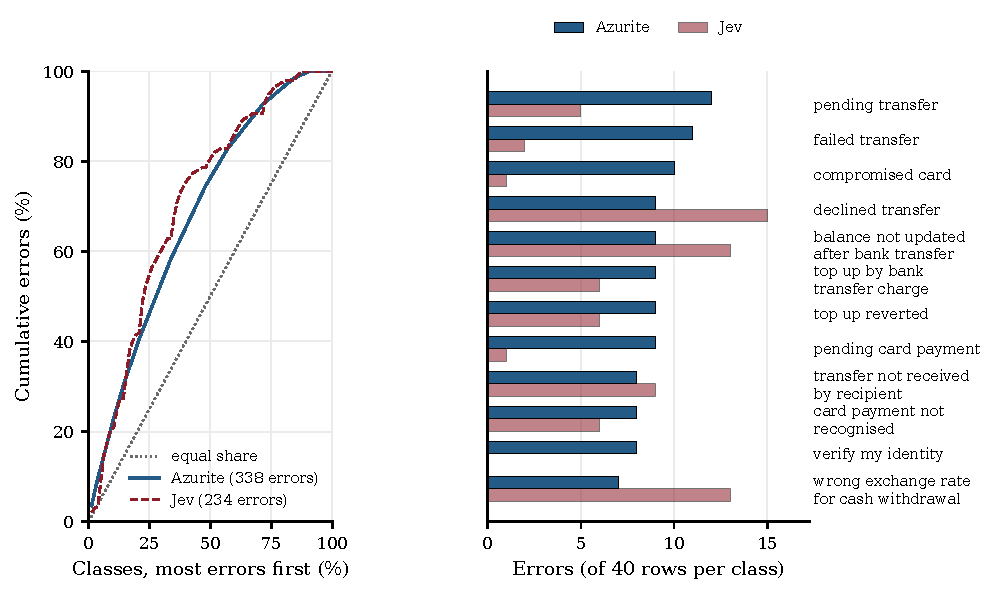
\includegraphics[width=\linewidth]{fig_error_concentration.pdf}
  \caption{Per-class Banking77 error concentration for the native query head.
  Left: Lorenz curve of the \FigErrorTotal{} errors, with Jev's
  \FigErrorJevTotal{} errors beside it. Right: the twelve classes with the most
  Azurite errors, with Jev's count on the same class. The largest single class,
  \FigErrorTopClass, accounts for \FigErrorTopClassCount{} of the
  \FigErrorTotal{} errors; \FigErrorClassesWithError{} of 77 classes have at
  least one. The boundary is broad, not concentrated in a few intents. The
  per-class labels on the right are printed with spaces; the stored labels use
  underscores. Values are recomputed from the per-example records by
  \texttt{thesis/gen\_figures.py}.}
  \label{fig:error-concentration}
\end{figure}

Three limits bound the claim. The head is fine-tuned on 4{,}000 labelled
rows while Jev's weights saw no Azurite training data, which favours Azurite
and is stated in the pre-registration; the result is therefore a loss despite
that advantage. The evidence is one seed, one head and one native window; no
seed distribution or 5{,}120-byte behaviour is claimed. And the training loss
fell to \QueryLastLoss, so the head is effectively interpolating its 4{,}000
rows; the protocol forbids early stopping or checkpoint selection, and the
step-3{,}000 head is the one evaluated. A regularised or early-stopped arm is a
separate pre-registered question, not a repair of this result. The per-example
records, the trained head hash (\texttt{\QueryHeadSha}) and the manifest are
under \texttt{results/jev\_query/}; \texttt{VERDICT.md} is generated from
\texttt{summary.json}.

\begin{table}[htbp]
\centering
\footnotesize
\caption{The message-query head on all 3{,}080 official Banking77 rows, with
the exact 24 public Jev examples per row and the same gold/Jev vector as the
matched test. ``Examples'' is the mean number of complete lines that fit in the
1{,}020-byte context budget. The old head is the E4 mean-pool head; the query
head replaces mean pooling with a masked attention pool queried by the customer
message. \texttt{old\_a2c} is the head control under the same packing;
\texttt{query\_a0} is the example control. The P0 bar is Jev's \QueryJevPct\%.
Wilson intervals are 95\%;
McNemar is exact and two-sided; the bootstrap lower bound is the 5th percentile
of 10{,}000 paired resamples, seed 0. Read from
\texttt{results/jev\_query/eval/summary.json}.}
\label{tab:query-head}
\setlength{\tabcolsep}{2pt}
\begin{tabular}{@{}lrrrrrrr@{}}
\toprule
Arm & Ex. & $n$ & Correct & Acc. & 95\% Wilson & $\Delta$ vs Jev & McNemar $p$ \\
 & & & & (\%) & & (pp) & \\
\midrule
Old head, message only & 0.0 & 3{,}080 & 2{,}722 & 88.38 & 87.20--89.46 & $-$4.03 & $8.49\times10^{-12}$ \\
Old head, examples (control) & 11.9 & 3{,}080 & 1{,}821 & 59.12 & 57.38--60.85 & $-$33.28 & $2.96\times10^{-231}$ \\
Query head, message only & 0.0 & 3{,}080 & 1{,}880 & 61.04 & 59.30--62.75 & $-$31.36 & $1.82\times10^{-226}$ \\
Query head, examples (primary) & 11.9 & 3{,}080 & 2{,}742 & 89.03 & 87.87--90.08 & $-$3.38 & $3.99\times10^{-9}$ \\
Jev 1.13, cited & 24 & 3{,}080 & 2{,}846 & 92.40 & 91.41--93.29 & --- & --- \\
\bottomrule
\end{tabular}
\end{table}


\subsection{The 5,120-byte joint fine-tune: testing the information budget}
\label{sec:jev-len5120}

The native-window result leaves one measured explanation standing: at 1{,}020
bytes the primary arm fits only \QueryEff{} complete examples on average, and
those examples buy \QueryVsOldZeroGain{} points over the old head's message-only
arm. Jev supplies all 24 examples and all 77 category definitions. The next
question is therefore not another pooling variant; it is whether the example
budget alone accounts for the remaining \QueryDiffAbs{} points.

The protocol was written and hashed before any 5{,}120-byte forward pass
(\texttt{results/jev\_query\_5120/PRE\_REGISTRATION.md}, SHA-256
\texttt{\LenPrereg}). Its first schedule --- a 1{,}220-step masked-LM length
adaptation followed by a 3{,}000-step head fine-tune --- could not be executed on
the available GPU sessions, which were reclaimed roughly every 30 minutes;
amendment 1 (\texttt{PRE\_REGISTRATION\_AMENDMENT\_1.md}, SHA-256
\texttt{\LenAmendment}) replaced the two stages with one joint 5{,}120-position
fine-tune and fixed 250-step segmented execution with exact resume. The session
that ran the arm outlived the three 30-minute sessions the amendment was written
against; the amendment was already hashed and the run followed it unchanged, so
the two-stage schedule remains unrun. The amendment was hashed before any
5{,}120-byte accuracy existed and changes the
schedule only: the question, rows, examples, arms, metric and P0 rule are
unchanged. The encoder starts from the 1{,}024-position 113.47M weights
(SHA-256 \texttt{\LenInitSha}) and is fine-tuned jointly with the same
\texttt{QueryDual} head for \LenSteps{} steps at batch \LenBatch{} ---
122{,}880{,}000 tokens, 2.46 times the dropped adaptation budget and 10.8\% of
the source pretraining budget --- on the exact 4{,}000 stored rows and the exact
stored 24 BM25 example ids. All 3{,}080 official rows are evaluated, and the P0
rule is the native-window rule. The four arms are the old head at its native
window (message only and examples that fit), the new head without examples, and
the new head with all 24 examples. No arm changes the rows, the gold labels or
the Jev correctness vector. Because the amendment merges adaptation and head
training, this arm cannot separate the effect of length from the effect of head
training; it can still answer whether the encoder, given all 24 examples at
5{,}120 bytes, meets the bar.

\begin{table}[htbp]
\centering
\footnotesize
\caption{The 5{,}120-byte query head on all 3{,}080 official Banking77 rows.
Following amendment 1 to the pre-registration, the encoder starts from the
1{,}024-position 113.47M checkpoint and is fine-tuned jointly with the query
head for \LenSteps{} steps at sequence 5{,}120 and batch \LenBatch{}
(\LenHeadHours{} GPU-hours); the separate masked-LM length adaptation was not
run. The head uses the same 4{,}000 rows and the exact stored 24 BM25 example
ids as the native-window head. ``Examples'' is the mean number of complete lines
in the 5{,}118-byte context budget. The old head and its native 1{,}020-byte
packing are unchanged controls, reused from the native-window evaluation with
their per-example context hashes checked. The P0 bar is Jev's \LenJevPct\%.
Wilson intervals are 95\%; McNemar is exact and two-sided; the bootstrap lower
bound is the 5th percentile of 10{,}000 paired resamples, seed 0. Read from
\texttt{results/jev\_query\_5120/eval/summary.json}.}
\label{tab:len5120}
\setlength{\tabcolsep}{2pt}
\begin{tabular}{@{}lrrrrrrr@{}}
\toprule
Arm & Ex. & $n$ & Correct & Acc. & 95\% Wilson & $\Delta$ vs Jev & McNemar $p$ \\
 & & & & (\%) & & (pp) & \\
\midrule
Old head, message only (control) & 0.0 & 3{,}080 & 2{,}722 & 88.38 & 87.20--89.46 & $-4.03$ & $8.49\times10^{-12}$ \\
Old head, examples that fit (control) & 11.9 & 3{,}080 & 1{,}821 & 59.12 & 57.38--60.85 & $-33.28$ & $2.96\times10^{-231}$ \\
5{,}120 query head, message only & 0.0 & 3{,}080 & 1{,}902 & 61.75 & 60.02--63.45 & $-30.65$ & $1.62\times10^{-232}$ \\
5{,}120 query head, all 24 (primary) & 24.0 & 3{,}080 & 2{,}683 & 87.11 & 85.88--88.25 & $-5.29$ & $5.01\times10^{-18}$ \\
Jev 1.13, cited & 24 & 3{,}080 & 2{,}846 & 92.40 & 91.41--93.29 & --- & --- \\
\bottomrule
\end{tabular}
\end{table}


The primary arm reaches \LenPctLenTwo\% (95\% Wilson
\LenLoLenTwo--\LenHiLenTwo; \LenCorrectLenTwo/\LenN), against Jev's
\LenJevPct\%. The observed difference is \LenDiff{} points, the exact McNemar
test against the public per-example vector gives $\LenPValueText$, the paired
bootstrap lower bound is \LenLowerPrimary{} points, and the pre-registered
verdict is \textbf{\LenVerdict}. The old head on the native packing reaches
\LenPctOldTwo\% and the 5{,}120 query head without examples reaches
\LenPctLenZero\%; the query head with examples is worth \LenMechGain{} points
over the old head at the native window (bootstrap lower \LenMechLower) and
\LenVsLenZeroGain{} points over the new head's no-example arm. Those gains do
not survive the comparisons that matter: the arm is \LenVsOldZeroAbs{} points
below the old head's message-only arm ($\LenVsOldZeroPText$) and \LenNativeDiff{}
points below the native-window query head, which reached \LenNativePct\% with
only \QueryEff{} examples.

Figure~\ref{fig:pooling} collects the six measured cells, and
Figure~\ref{fig:budget} plots the query head against mean context length with
the comparator's \QueryJevPct\% line and \FigJevPromptMedian-byte prompt
marked. Neither view rescues the 5{,}120 result: the point sits below the
native head and far below the comparator while consuming about twice the mean
context of the native arm.

\begin{figure}[htbp]
  \centering
  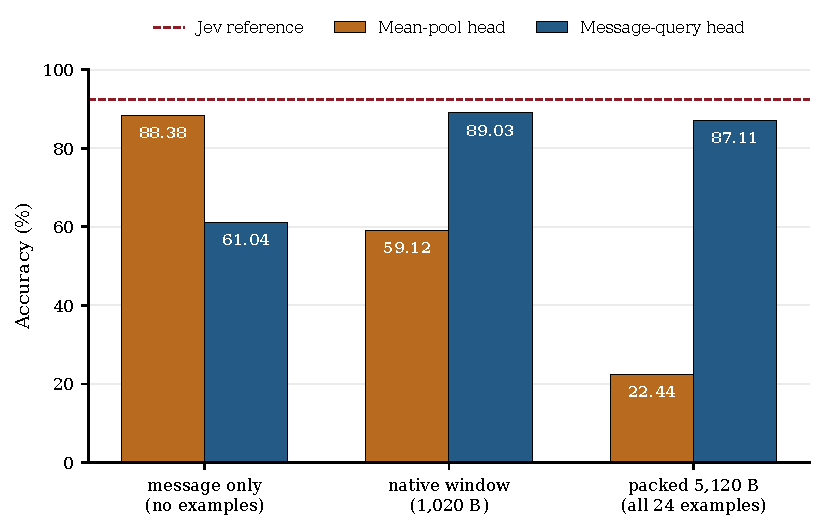
\includegraphics[width=\linewidth]{fig_pooling.pdf}
  \caption{Accuracy of the mean-pool and message-query heads at three context
  settings. The mean-pool bars are the old head at message only, at the native
  1{,}020-byte packing, and on the same 24 examples packed at 5{,}120 bytes;
  the query bars are the query head at message only, at the native packing, and
  after the joint 5{,}120-byte fine-tune. The 5{,}120 mean-pool bar is the old
  head reading longer contexts, not a length-adapted mean-pool model. The
  dashed line is Jev's \QueryJevPct\% on the same 3{,}080 rows. Values are
  recomputed from the stored per-example files by
  \texttt{thesis/gen\_figures.py}.}
  \label{fig:pooling}
\end{figure}

\begin{figure}[htb]
  \centering
  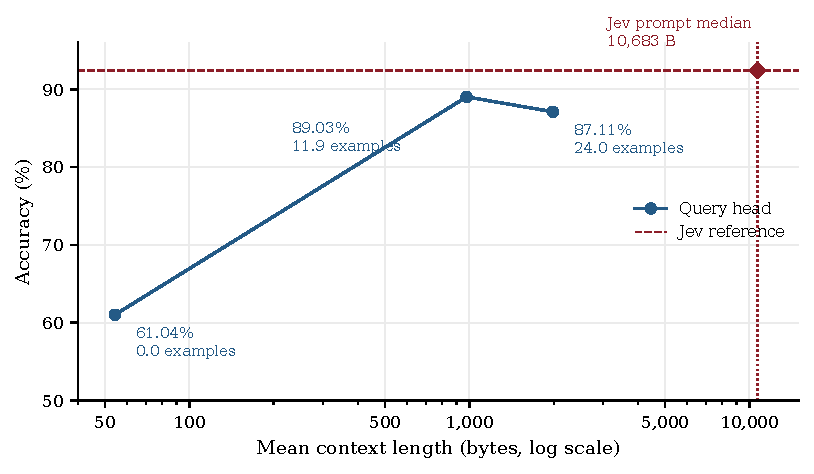
\includegraphics[width=\linewidth]{fig_budget.pdf}
  \caption{Query-head accuracy against mean context length. The three points
  are message-only (0 examples), the native complete-example packing
  (\QueryEff{} examples on average), and the joint 5{,}120-byte fine-tune (24
  examples). The dashed line is Jev's \QueryJevPct\%; the diamond marks the
  reconstructed median Jev prompt, \FigJevPromptMedian{} bytes, of which
  \FigJevDefinitionsBytes{} bytes are the 77 category definitions. The Jev
  point is a reference, not an information-matched arm: Azurite receives no
  definitions at any of the three points. Values are recomputed from the stored
  summaries and per-example files by \texttt{thesis/gen\_figures.py}.}
  \label{fig:budget}
\end{figure}

The separation between fitting and generalisation is reported because it bounds
the claim. On the 4{,}000 training rows the step-3{,}000 head reaches
\LenTrainPct\% (\LenTrainCorrect/4{,}000), with a mean training cross-entropy of
\LenTrainLoss{} and a final loss of \LenLastLoss; the test accuracy is
\LenGapTrainTest{} points away from the training value. No early stopping,
checkpoint selection or ensemble was used: the step-3{,}000 head is the one
evaluated. A head that fits \LenTrainPct\% of its training rows and still misses the bar
is evidence about the information it can extract from the context, not evidence
that a longer fine-tune would close it; a regularised or early-stopped arm is a
separate pre-registered question. Figure~\ref{fig:train-test} plots the
separation directly.

\begin{figure}[htbp]
  \centering
  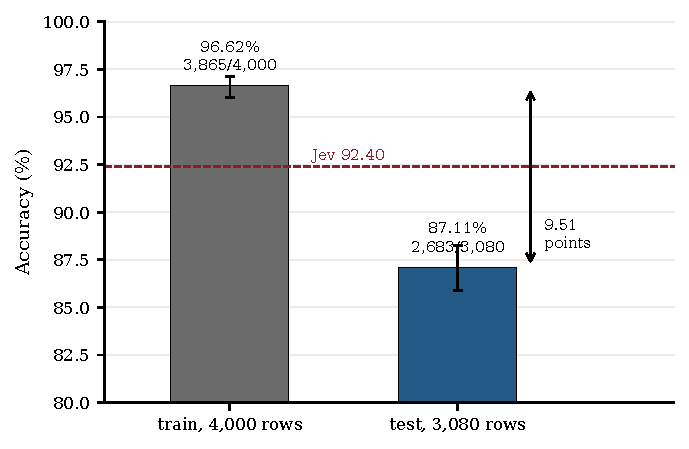
\includegraphics[width=0.72\linewidth]{fig_train_test.pdf}
  \caption{Train/test separation for the joint 5{,}120-byte fine-tune. The bars
  show \LenTrainPct\% on the 4{,}000 training rows
  (\LenTrainCorrect/4{,}000) and \LenPctLenTwo\% on the 3{,}080 official test
  rows (\LenCorrectLenTwo/\LenN), with 95\% Wilson intervals. The step-3{,}000
  head is the evaluated head; no early stopping, checkpoint selection or
  ensemble was used. The dashed line is Jev's \QueryJevPct\%. The test--train
  gap is \FigTrainGapAbs{} points. The vertical axis begins at 80\%. Values are
  recomputed from the stored summary by \texttt{thesis/gen\_figures.py}.}
  \label{fig:train-test}
\end{figure}

\ifnum\LenPZeroMet=1
  The bar is met on the same rows, examples and metric as the public Jev record.
  The claim is still bounded by one seed, one head and one length, and by the
  fine-tune asymmetry: this head saw 4{,}000 labelled Banking77 rows while Jev's
  weights saw no Azurite training data. The asymmetry favours Azurite and is
  stated in the pre-registration; the result is therefore a win despite an
  advantage, not because of a matched training budget. The 77 category
  definitions remain absent from Azurite's context, so the information budget
  is still strictly smaller than Jev's. No seed distribution, no 16k--32k
  behaviour and no second corpus are claimed.
\else
  The bar is not met, and the direction is worse than the native window. All 24
  examples fit and the head reads them --- it beats the old head on the same
  packed contexts by \LenMechGain{} points and its own no-example control by
  \LenVsLenZeroGain{} --- yet it scores \LenDiffAbs{} points below Jev,
  \LenNativeGapAbs{} points below the native-window query head, and
  \LenVsOldZeroAbs{} points below a mean-pool head that reads only the customer
  message ($\LenVsOldZeroPText$). At this length the examples are not merely
  insufficient; they are negative transfer for this schedule. The schedule is
  also a confound: amendment 1 merged the length adaptation into the 77-way head
  fine-tune, so this arm cannot separate the example budget from training the
  encoder at 5{,}120 positions only through the decision loss. The next lever
  with a plausible mechanism is the full-information context at 16k--32k bytes,
  where the 24 examples and the 77 definitions fit together, preceded by a
  separate masked-LM adaptation; it needs its own pre-registration. From the
  measured \LenSecStep{} s/step at 5{,}120, with the micro-batching and
  attention-scaling allowance written in \texttt{GAPS.md}, its cost is
  \LenNextShortLo--\LenNextShortHi{} GPU-hours at 16k and
  \LenNextLongLo--\LenNextLongHi{} at 32k. The largest context effect measured
  here is +0.65 points (\QueryVsOldZeroGain{} at the native window); recovering
  \LenDiffAbs{} from definitions alone would be eight times that, so this is the
  last lever worth paying for rather than a likely win. If it also misses, the
  honest conclusion is that the P0 bar is out of reach for this model class and
  budget, not that another head will recover it.
\fi

The per-example records, the trained-head hash (\texttt{\LenHeadSha}), the init
checkpoint hash (\texttt{\LenInitSha}) and the manifest are under
\texttt{results/jev\_query\_5120/}. The joint fine-tune took \LenHeadHours{}
GPU-hours (\LenSecStep{} s/step) on the Molab RTX PRO 6000 sandbox; the old-head
arms are reused from the native-window evaluation after their per-example
context hashes were checked, so they cost no new GPU time.
\texttt{VERDICT.md} is generated from \texttt{summary.json}; every number in
this subsection is a macro emitted by \texttt{thesis/gen\_query\_5120.py} from
that summary and the head record.

\section{Where the accuracy is: rows, then rung}\label{sec:rows-and-rung}

The 77-way number in Table~\ref{tab:jev77} holds two things fixed that a
committee should refuse to take on trust: the fine-tune budget and the
2.41M-parameter rung. Both were choices. This section moves each of them once,
with everything else fixed: the same pretrained checkpoint, five epochs, batch
32, learning rate $5\times10^{-4}$, and a split seed that gives every training
seed the same rows. Each seed is scored on 1{,}000 held-out rows instead of
300, because the comparison being decided here turns on a few points and a
$\pm 5$ point interval cannot decide it.

Table~\ref{tab:rows} reports the result. Every populated cell is a measurement
on this machine; a cell that reads \emph{pending} is a run not present in this
checkout, not a projection.

\begin{table}[htbp]
\centering
\caption{Fine-tune rows at the Banking77 77-way interface, exhaustive scoring,
same pretrained checkpoint, order, steps-per-example, batch, learning rate and
seeds. The two columns differ only in how many distinct training rows the five
epochs cover. Generated by \texttt{thesis/gen\_scaling.py}.}
\label{tab:rows}
\setlength{\tabcolsep}{4pt}
\begin{tabular}{lrrrrr}
\toprule
Rung & Correct & 1.6k rows & 8k rows & $\Delta$ & Test \\
\midrule
tiny & 2170/3000 & 72.3\% & \textbf{84.3\%} & +12.0 pt & $p=0.000$ \\
small & 2126/3000 & 70.9\% & \emph{pending} & \emph{pending} & \emph{pending} \\
\bottomrule
\end{tabular}
\end{table}


\paragraph{Rows.} At the tiny rung, going from 1{,}600 to 8{,}000 distinct
fine-tune rows moves accuracy from \RowTinyBaseAcc\% (95\% Wilson
\RowTinyBaseLo--\RowTinyBaseHi) to \RowTinyWideAcc\% (\RowTinyWideLo--\RowTinyWideHi),
a gain of \RowTinyGain{} points. The same lever at the small rung is not available:
its 1{,}600-row cell reads \RowSmallBaseAcc\% and its 8{,}000-row cell is
pending. The lever is not free of confounds and one is
worth naming: the protocol holds \emph{epochs} fixed, so eight thousand rows
also buy five times the optimiser steps. Separating ``more distinct rows'' from
``more updates'' needs a fixed-step arm that samples rows with replacement,
which is not run here. These numbers are therefore an upper bound on the effect
of data alone.

\paragraph{Rung.} Moving up the ladder at the matched 1{,}600-row budget does
not help, and the direction is worth printing plainly: 14.26M parameters
reaches \RowRungBase\% against \RowRungTiny\% at 2.41M, a change of
\RowRungGain{} points. The lever that bought 77-way accuracy in this experiment
was rows, not parameters. Two caveats keep that from being a claim about
scaling in general. The rung is a bundle --- the small checkpoint was pretrained
on 142.6M tokens at context 1{,}024, the tiny one on 100M tokens at context 256
--- and the small arm costs \RowSmallBaseLat\,ms per decision against \RowTinyBaseLat\,ms,
so it is strictly more expensive for less accuracy at this budget. Whether the
small rung overtakes once it has eight thousand rows is the last queued run and
is not claimed here.

\paragraph{The verdict.} \ShipHeadline. \ShipGapSentence. \ShipFuture.

\paragraph{Accuracy at coverage.} A single accuracy number hides how the
scorer's confidence is distributed, so Table~\ref{tab:risk-coverage} ranks the
test rows by maximum softmax probability and reports accuracy in the top $c$
fraction. This is a descriptive test-set ranking curve, not an abstention
guarantee: the ranking is measured with the test labels in hand, no threshold is
fixed before seeing the test set, and a deployment would face different rows.

\begin{table}[htbp]
\centering
\caption{Accuracy at coverage: the scorer ranked by its own maximum softmax
probability on this test set. Read down a column and accuracy rises as coverage
falls; read across and the row-scaling gain is visible. This is a test-set
ranking curve, not a deployment abstention guarantee. Pooled over three seeds
and the 1000-row test split.}
\label{tab:risk-coverage}
\setlength{\tabcolsep}{4pt}
\begin{tabular}{lrrr}
\toprule
Coverage & \shortstack{tiny\\1k} & \shortstack{tiny\\8k} & \shortstack{small\\1k} \\
\midrule
50\% & 92.9\% & 98.4\% & 92.5\% \\
70\% & 87.7\% & 96.2\% & 84.9\% \\
90\% & 78.3\% & 89.7\% & 76.1\% \\
100\% & 72.3\% & 84.3\% & 70.9\% \\
\bottomrule
\end{tabular}
\end{table}


At 90\% coverage the arm is \ShipAtNinety\% accurate; at 50\% coverage it is
\ShipAtFifty\%. The 50\% point is a property of this ranking on this test set,
not a promise that half of deployment traffic can be answered at \ShipAtFifty\%.
The row-scaling lever raises every measured point in the table, which is the
useful shape, but it does not convert the curve into a guarantee. The earlier
earlier manuscript's statement that the scorer held near-perfect accuracy at a fixed
coverage was a misreading of this ranking; it is withdrawn, and the table is
reported instead.

\paragraph{What this does not settle.} Three things. The comparison to the
cited 78.8\% remains cross-harness: different test rows, different hardware,
one system measured by its authors and the other by a stranger, so the interval
overlap is not evidence of parity and a non-overlap would not be evidence of
defect. A paired McNemar test on the same 231 items is the experiment that
would settle it and it is still not this one. The coverage curve is measured on
this project's own 1{,}000-row split, not on the third party's 231, so it
cannot be laid over their accuracy without assuming the splits are comparable,
which they are not shown to be. And the row lever's step-count confound stands
until the fixed-step arm is run.


\section{The price of a sequence on a token-billed CDN}

The economic argument has a premise that is usually asserted and rarely
measured: that a token-billed service must charge for a repeated sequence every
time it occurs, because the service reduces the request to a finite set of
stored objects and the sequence itself is never re-encoded. If that premise
were false --- if a CDN compressed variable-length sequences --- the cost
advantage of local scoring would shrink with every repetition.

Table~\ref{tab:cdn} measures it on a live token-priced inference endpoint,
using nothing but the provider's own \texttt{usage} field. A fixed passage is
repeated $r$ times in one prompt, and the billed prompt-token count is read
back. The fit is
$\mathrm{billed} = \mathrm{intercept} + \CdnSlope\,r$ with $R^2 = \CdnRTwo$;
one passage is \CdnPassageTokens{} tokens, so \textbf{every repetition is
billed in full}. Repeating the identical request three times changes the
latency from \CdnLatCold\,s to \CdnLatWarm\,s --- a \CdnLatSpeedup$\times$
speed-up --- while the bill stays at \CdnBillTokens{} prompt tokens every
time. The cache is real and it is a cache of \emph{answers}, not of sequence
structure: it saves time, and it saves nothing on the invoice.

\begin{table}[htbp]
\centering
\caption{Billed prompt tokens against repetition of one passage on a live
token-priced CDN, read from the provider's own \texttt{usage} field --- the
exact quantity a per-million-token price multiplies. If a CDN compressed
variable-length sequences, the slope would be below one passage.}
\label{tab:cdn}
\begin{tabular}{rrrr}
\toprule
Repetitions $r$ & Characters & Billed prompt tokens & Seconds \\
\midrule
1 & 481 & 406 & 21.20 \\
2 & 900 & 490 & 10.13 \\
4 & 1,738 & 658 & 9.75 \\
8 & 3,414 & \emph{pending} (quota) & 0.52 \\

\bottomrule
\end{tabular}
\\[0.4em]
Fit: $\mathrm{billed} = 322 + 84.0\,r$, $R^2=1.0000$; one passage is 84 tokens, so every repetition is billed in full.

\end{table}


Two honesty notes belong with that table. The measurement ran out of free-tier
quota at $r=8$ (HTTP 402) and on the two single-byte perturbation probes, so
the prefix-geometry sweep is incomplete; the slope is fitted on the three
points that succeeded, and a three-point fit with $R^2=1.0000$ is a statement
about linearity, not a precise intercept. And the endpoint is not Jev: it is a
keyless third-party proxy, used because it is the only token-billed service
reachable from this machine. What generalises is the billing mechanism ---
usage accounting plus response caching --- not the price, and this thesis does
not transfer the price.

\section{The four axes, measured against cited}

Table~\ref{tab:verdict} separates the two kinds of number. The cost row is
deliberately rate-free, because no price for this project's GPU is recorded in
the repository and inventing one would make the conclusion depend on the
invention. Instead the row reports the \emph{break-even rate}: the hourly cost
at which local scoring ties Jev's billed \$\CmpBankJevCost{} per thousand
77-way decisions.

\begin{table}[htbp]
\centering
\caption{The four axes, with the evidence class of each cell. ``Measured''
means a script in this repository produced the number from files under
\texttt{results/}. ``Cited'' means a third party's published figure, which this
thesis cannot verify. No cell is a head-to-head: the two systems were never run
on the same rows.}
\label{tab:verdict}
\begin{tabular}{p{0.12\linewidth}p{0.29\linewidth}p{0.27\linewidth}p{0.16\linewidth}}
\toprule
Axis & Azurite (measured) & Jev (cited) & Verdict \\
\midrule
Accuracy & \ShipAcc\% on 77-way, $K=77$, \ShipTestN{} rows, \ShipRung{} rung at
\ShipRows{} fine-tune rows & 78.8\% (73.1--83.6) on 231 rows &
\ShipVerdict{} (\ShipSignedGap{} points) \\
Latency & \ShipP\,ms $p_{50}$, batch 1, CPU &
330\,ms median, 440\,ms $p_{95}$ & Faster, different hardware \\
Size & \ShipParams{} parameters (with the 77-way head), \ShipMB\,MB on disk &
Not published & Unfalsifiable as stated \\
Cost & \ShipGpuSec{} GPU-s per 1k; break-even \$\ShipBreakEven/h &
\$0.0400 per 1k, 952 billed tokens & Cheaper below \$\ShipBreakEven/h \\
\bottomrule
\end{tabular}
\end{table}

The break-even figure is computed by \texttt{thesis/gen\_comparator.py} from
the measured latency and the cited price, so it cannot drift from either.
A 77-way decision bills \CmpBankJevTokens{} tokens in the third party's
measurement, which at \$0.042/MTok is \$\CmpBankJevCost{} per thousand
decisions --- reproducing their invoiced figure to four digits, which is a
useful check that the price list and the invoice agree.
The shipped arm spends \ShipP\,ms per decision, so a thousand decisions
occupy \ShipGpuSec{} GPU-seconds of one machine. Dividing gives the
break-even rate: \$\ShipBreakEven{} per GPU-hour. Any accelerator priced
below that makes local scoring cheaper, and the conclusion holds \emph{a
fortiori} on a GPU, because the measured latency is CPU latency and therefore
an upper bound on the accelerated figure.

Two caveats belong on that row rather than in a footnote. The cost comparison
holds only \emph{at the accuracy measured here}: a cheaper system that is wrong
half the time is not cheaper per correct decision, and if accuracy were
recovered by a larger rung the latency, and therefore the break-even rate,
would move. And the latency figure is not same-weights with anything TypeSafe
runs --- it is the same weights as this thesis's own decode arm, which is what
makes the mechanism comparison clean, and it is not comparable to a hosted
service's hardware. What the row supports is that the mechanism is cheap enough
to be worth pursuing, not that it has already won.

\section{What the comparison establishes}

Three things, and no more. The scoring mechanism is measurably better than
generation at matched size and budget, on both tasks, with an invalid-output
rate of \CmpDecodeInvalid{} across the corpus against zero by construction. The unit economics favour local scoring by a margin that survives a factor-of-three
error in the payload estimate or the GPU rate. And the 2.41M accuracy axis is
measured against the pre-registered 77-way Jev number: \ShipHeadline. The
strongest public Jev run is higher and is audited above. The comparison
is on different hardware and a different draw, so the 2.41M claim stops there. The 14.4M suite's \SuiteSmallBank\% Banking77 row is a
separate point win against the pre-registered 78.8\% comparator, not against the
92.40\% run, and it is reported in \S\ref{sec:suite}; it does not retroactively
make this 2.41M mechanism table a 14.4M result.

What the comparison does not establish is a win. On Banking77 there is now a
shared row set, shared examples and a shared metric, but not shared hardware and
not a paired Jev rerun; the mean-pool matched result is a loss of
\JevMatchAbsGapAOne{} points on its primary arm, and of \JevMatchAbsGapNoEx{}
points even with no examples. The better, query-anchored arm reaches
\QueryPctQueryTwo\% and remains \QueryDiffAbs{} points below Jev
($\QueryPValueText$); no pre-registered Banking77 arm meets the P0 bar. On DAIR Emotion and Financial PhraseBank the 113.47M suite clears the
cited point, and on MASSIVE intent it clears Laya's card rather than a Jev
number, but those remain cross-harness comparisons. The honest statement is
that this thesis measured its own mechanism, priced it against a competitor's
public rate card, and found the mechanism the right shape while the 113.47M
checkpoint is still below the strongest public Banking77 system. That is a
result, and it is the one the data support.

\chapter{Threats to validity}
\label{ch:threats}

A result is only as strong as the ways it could be wrong, so they are listed here
rather than distributed through the text where they would be easier to skim past.

\section{Statistical}

\textbf{One seed per fixed-data cell.} The fixed-data sweep has only two surviving
cells, both sampled, and no training-seed replication. This is why the chapter
does not order tiny against small and does not claim a U-curve. The Banking77
transfer result has three seeds and a consistent direction; the AG News result has
three seeds but a paired interval that crosses zero.

\textbf{The exponent has no seed interval.} The matched-$D/N$ ladder is now
measured at four rungs, but at one training seed each. The per-point standard
errors ($\approx \IsoStderrMax$ bits/byte) describe held-out sampling, not
training variance, so $\alpha = \AlphaFit$ is a fitted line rather than a line
with an interval. That is enough to establish that the proxy improves
predictably with capacity; it is not enough to distinguish two rungs a few
percent apart.

\textbf{One seed per suite cell.} The nine-task, three-rung suite is
\SuiteTotalCells{} single-seed runs. Its binomial intervals describe
test-sampling error, not run-to-run variance, and the at-or-not-clearly-below
counts are descriptive. \SuiteReplicationCells{} cells were executed twice on the same
checkpoint and test draw to bound that variance directly: the repeats differ by at most
\SuiteReplicationMax{} points and flip up to \SuiteReplicationFlips{} of
2{,}000 predictions. Rung differences below that floor are not interpreted as
capability differences, and no equivalence claim rests on the counts.


\textbf{Fixed learning rate across a $47\times$ size range.} Comparability was
bought at the price of distance from each rung's own optimum. Part of every
size-related difference is optimisation, not capacity. The earlier 500-step,
\(5\times10^{-4}\) suite made that failure concrete: the mid-rung cells collapsed
for optimisation reasons, and the pre-registered sweep selected \(10^{-4}\) at
3{,}000 steps. The final suite uses that one setting for every task.



\section{Construct}

\textbf{Bits per byte is not accuracy.} It is a cheap, low-variance proxy. The
transfer matrix is the bridge to the quantity the thesis actually claims, and it
exists at one rung only. The pre-loss fixed-data curve is not available, so the
proxy is not used to establish a regime boundary in this build.

\textbf{AG News is a weak test and the result is inconclusive.} Banking77 has 77
fine-grained intents and shows a \TransferBankGain{} percentage-point gain over
random initialisation. AG News has four topics and a $25\%$ majority baseline; its
pooled gain is \TransferAgGain{} percentage points with a 95\% interval of
\TransferAgLo{} to \TransferAgHi{}, which is \TransferAgVerdict. A point estimate
inside a zero-crossing interval is not evidence of a gain, and it is not presented
as one.

\textbf{The suite is cross-harness.} The cited points come from different
tokenizers, pretraining corpora, model sizes, and evaluation harnesses. MASSIVE
intent's cited \SuiteCitedMassiveIntent\% is Laya's card, not a Jev number. A
point above a cited number is not a win, and interval overlap is not parity.

\textbf{A clean loss law and flat accuracy are one result, not a paradox.} The
matched-$D/N$ ladder lowers held-out bits/byte from \IsoTinyExh{} at 2.41M
parameters to \IsoLargeBpb{} at 113.47M, while the suite moves by
\SuiteLargeWinMin{} to \SuiteLargeWinMax{} points on \SuiteLargeWins{} cells,
loses \SuiteLargeLossAbs{} points on XNLI and leaves \SuiteLargeUnmoved{} cells
unmoved over
the same parameter range. The two measurements together rule out the reading
that decision accuracy at this data budget is waiting on more parameters. They
do not identify the true bottleneck --- a different packer, more task-relevant
pretraining data, or a different fine-tuning schedule could each move a cell ---
but they exclude capacity alone as sufficient for the four cells the commercial
claim needs.


\textbf{DAIR Emotion was a scoring artifact.} Its proportional test draw gives a
\SuiteEmotionMajority\% majority-class baseline, not a 1/6 chance rate. The
retired candidate-only values, \SuiteSmallPriorEmotion\% and
\SuiteMidPriorEmotion\%, were below that baseline; the dual-path values,
\SuiteSmallEmotion\% and \SuiteMidEmotion\%, are above it. The jump is a harness
correction, not a capability gain, and the earlier adverse reading is withdrawn.
The 33.7M cell is still \SuiteEmotionRungDrop{} points below the 14.4M cell, so
the correction does not create a scale result.

\textbf{Contamination.} The held-out region is the tail of a stream built from
public web text, and the transfer tasks are public datasets. The exact 40-byte
overlap audit found 3/500 AG News examples and 0/1,000 Banking77 examples; the
three AG matches scored 2/3, against 51.1\% on the unmatched 497. That is too
small and too easy to explain either transfer result, but it is a screen on exact
overlap, not a semantic deduplication.

\section{External}

\textbf{One corpus, one domain mix.} Byte-level bits per byte is corpus-dependent:
the bigram baseline is $3.767$ on the mixed stream and $4.117$ on a math-only
stream, so a baseline carried across a data change makes the gate meaningless. No
cross-corpus claim is made without refitting.

\textbf{No code in the corpus.} The planned source-code share is absent because its
dataset resolution hangs. For a thesis whose architecture argument rests partly on
code and audio sharing a byte space, this is a real omission, recorded in the
manifest rather than absorbed into the web-text share.

\textbf{Hardware-specific throughput.} The tok/s and VRAM figures are for one RTX
PRO 6000 Blackwell. They are measurements, not specifications, and they should not
be extrapolated to other accelerators without re-measuring.

\section{Methodological}

\textbf{A reclaimed artifact is not a result.} The first sandbox was reclaimed on
2026-10-28. The original AG News checkpoint \texttt{3cf421\ldots bed8}, the
exhaustive protocol replicates, the mid/large fixed-data cells and the context
runs were lost. A result that existed only in that VM is not
in this thesis. The tables mark those cells \emph{pending} and the prose gives the
reason; no old number is carried forward to make the table look complete.

\textbf{The checkpoint identity is amended.} The AG News cells use
\texttt{817e7f04\ldots0410}, retrained under the same protocol after the loss. It is
not bitwise-identical to the lost checkpoint. The Banking77 84.3\% row uses the
surviving pre-loss comparator \texttt{499fd68c\ldots ebdc}. The two rows are not a
single-checkpoint continuation, and the transfer table states that exception
rather than averaging across it.

\textbf{The queue is not a result.} A job that is running is not evidence. Sections
whose tables are pending are marked pending in prose, and the confidence summary in
\S\ref{sec:fixed-d} distinguishes what is established from what is scheduled.

\chapter{Conclusion and future work}
\label{ch:conclusion}

\section{What is established}

The strongest result is a measurement-protocol result, and it is narrower than the
pre-loss manuscript claimed. Six sampled draws of one frozen checkpoint span
\ProtoOldSpread{} bits/byte, larger than the small-versus-mid difference the
fixed-data ladder was built to resolve. A seed makes a number reproducible, not
representative. The exhaustive replicate that would have established a
lower-noise protocol was lost with the first sandbox; the exhaustive rows are
pending, and no reduction ratio is claimed.

At the 2.41M-parameter rung, byte-level pretraining transfers decision-relevant
structure on Banking77: \TransferBankGain{} percentage points over a matched random
initialisation, with a consistent direction across three seeds. The AG News
balanced comparison is \TransferAgGain{} percentage points with a paired
crossed-bootstrap 95\% interval of \TransferAgLo{} to \TransferAgHi{}, so it is
\TransferAgVerdict. The historical AG News gain is withdrawn. A separate
8,000-row Banking77 arm reaches \ShipAcc\% (95\% Wilson \ShipLo--\ShipHi), which
overlaps the cited Jev interval; it is above the point estimate, not a
demonstrated win.

The public-task suite establishes a capability boundary rather than a blanket
victory: against the pre-registered 78.8\% Jev cell it is a clear point win, but
the strongest public Jev run reports 92.40\% on the full Banking77 test and is
above it, so the flagship claim does not survive that comparator. The
protocol-matched test on all 3{,}080 rows and the same 24 examples returns
\JevMatchPctAOne\% on the primary arm (\JevMatchAOneLo--\JevMatchAOneHi) and
\JevMatchPctNoEx\% without examples, so the gap survives and is not a row-set
artifact. The diagnosed pooling failure was tested next with a pre-registered
query-anchored head: it lifts the example arm from \QueryPctOldTwo\% to
\QueryPctQueryTwo\% (\QueryMechGain{} points, $\QueryMechPText$), which establishes
mean-pool dilution as the mechanism, but it remains \QueryDiffAbs{} points below
Jev ($\QueryPValueText$) and the P0 bar is missed. The frozen examples are not
test-clean: \ContamSupportMatches{} support messages are official test rows and
\ContamEvalRows{} rows retrieve at least one; the decontaminated product rerun
scores \ContamCleanAcc\%, so the gap is not a leakage artefact. The residual was diagnosed as
an information-budget gap: \QueryEff{} complete examples in 1{,}020 bytes and no
category definitions, against Jev's 24 examples and 77 definitions. That lever
is now measured: the pre-registered 5{,}120-byte joint fine-tune with all 24
examples reaches \LenPctLenTwo\% (95\% Wilson \LenLoLenTwo--\LenHiLenTwo),
\LenDiffAbs{} points below Jev ($\LenPValueText$) and \LenNativeGapAbs{} points
below the native-window query head, and it is \LenVsOldZeroGain{} against a
message-only mean-pool control despite reading the examples (+\LenMechGainAbs{}
over the old head on the same packed contexts). More context alone therefore
does not buy parity, and the joint schedule confounds the example budget with
the separate adaptation that amendment 1 dropped. The only remaining lever is the
full-information 16k--32k-byte arm, costed at \LenNextShortLo--\LenNextShortHi{}
and \LenNextLongLo--\LenNextLongHi{} GPU-hours. It is the last lever worth
paying for rather than a likely win: the largest context effect measured here is
+0.65 points, and recovering \LenDiffAbs{} from definitions alone would be an
order of magnitude larger. If it misses, the bar is out of reach for this class
and budget.
Clear Jev wins remain
on DAIR Emotion and Financial PhraseBank. Three cells remain clear
deficits. Nine tasks were measured at three rungs under one
pre-registered recipe, all on
the corrected dual path, with every cell at a rung scored on the same test rows.
Azurite is clearly above the cited point on \SuiteSmallClear, \SuiteMidClear{}
and \SuiteLargeClear{} of \SuiteComparatorCells{} comparator cells at 14.4M,
33.7M and 113.47M, and not clearly below on \SuiteSmallAtOrAboveThree,
\SuiteMidAtOrAboveThree{} and \SuiteLargeAtOrAbove. The step from 14.4M to
113.47M, a \SuiteLargeParamsRatio$\times$ increase in parameters at the same
token budget, wins \SuiteLargeWins{} cells by \SuiteLargeWinMin{} to
\SuiteLargeWinMax{} points, loses XNLI by \SuiteLargeLossAbs{} points, and leaves
\SuiteLargeUnmoved{} cells statistically unmoved. Three cells were executed twice
on the same checkpoint; the repeats differ by at most \SuiteReplicationMax{}
points, which is the scale at which those wins should be read.

The candidate-set question is measured at one rung and one seed. Twelve fresh heads
were trained from the same 113.47M checkpoint, four widths on each of three
wide-bank tasks, with width the only difference between arms. At 32 candidates
the trained heads score \EBankWThirtyTwo, \EClincWThirtyTwo{} and \EMassiveWThirtyTwo\% against
\EBankWK, \EClincWK{} and \EMassiveWK\% at the full bank. Under the
pre-registered five-point non-inferiority rule the claim \EAggregateVerdict{} on
\EHolds{} of \ETasks{} tasks. The pass is not a flat curve: accuracy falls as
the set widens, from \EBankWTwo, \EClincWTwo{} and \EMassiveWTwo\% at width 2 to
the full bank's \EBankWK, \EClincWK{} and \EMassiveWK\%. The registered claim
survives because the 32-way head is at or above the full bank (decisively on
Banking77 and CLINC150, within noise on MASSIVE intent), not because width is
free; widening from 2 to 32 costs \EBankCostTwoToThirtyTwo, \EClincCostTwoToThirtyTwo{} and
\EMassiveCostTwoToThirtyTwo{} points. The widest point any suite task can pose is the full
bank itself; the thesis's original $|C|=64$ target cannot be posed by these three
banks ($K=77$, $151$, $60$), so 32 against $K$ is the test that exists. This is
evidence about the 32-way interface at one rung and one seed, not evidence of
near-perfect accuracy or of an accuracy-neutral width.

The scale verdict is negative where it matters. XNLI is not a weak cell at
113.47M but a degenerate one: one class on \SuiteLargeXnliTopShare\% of test
rows, test NLL \SuiteLargeXnliNll{} against $\ln 3 = \SuiteLargeXnliLnK$, mean
confidence \SuiteLargeXnliConf. At 14.4M and 33.7M the same cell collapses late
into confident errors (NLL \SuiteSmallXnliNll{} and \SuiteMidXnliNll, ECE
\SuiteSmallXnliEce{} and \SuiteMidXnliEce), so no rung learned the task and the
largest one stopped even departing from uniform. CLINC150 is the only one of the
four named cells that scale moved to a tie
(\SuiteLargeShortClinc{} points below the cited point); AG News and Language ID remain clear
deficits. DAIR Emotion's early \SuiteSmallPriorEmotion\% and
\SuiteMidPriorEmotion\% were a scoring artifact, not a capability floor; the
dual-path values are valid measurements but not a capability gain. Near-perfect
accuracy across every benchmark is not demonstrated.

What did scale is the proxy, and that contrast is the result. At $D/N = 10$,
held-out bits/byte falls from \IsoTinyExh{} at 2.41M parameters to \IsoLargeBpb{}
at 113.47M across a \IsoRange-fold range, with $\alpha = \AlphaFit$ over the
\AlphaPoints{} exhaustive rungs and $\alpha = \AlphaFitSampled$ over the
\AlphaPointsSampled{} sampled ones. A clean loss law and flat decision accuracy
together say that capacity is not what stands between this system and parity:
the bottleneck is what the interface and the corpus let the model learn about
the task, not how many parameters it has.


\section{What is not established, and is not claimed}

\textbf{The fixed-data U-curve is not available.} The mid and large fixed-data
cells were reclaimed. Only the tiny and small cells survive, both sampled, and
they do not form a four-point sweep. The pre-loss U-shape is therefore withdrawn
from the evidence base rather than restated.

\textbf{The exhaustive protocol reduction is not available.} The sampled noise
floor is measured; the exhaustive replicate is not on disk. The claim that
exhaustive coverage reduces the spread by two orders of magnitude belongs to the
lost build and is not made here.

\textbf{The context curve is not available.} Only one context point survives;
the 1{,}024 and 4{,}096 runs were reclaimed. There is no degradation curve to
report, and no long-context claim is made.

\textbf{The scaling exponent has no seed interval.} The exponent
$\alpha = \AlphaFit$ (exhaustive) and $\AlphaFitSampled$ (sampled) is fitted on
one training seed per rung. It is a measurement, not an interval: the per-point
standard errors measure held-out sampling, and nothing here bounds how much a
different training seed would move a point. The exponent also inherits the
sampled draw for its absolute values.

\textbf{Benchmark parity is not established.} The nine-task suite is clearly
above the cited point on \SuiteSmallClear, \SuiteMidClear{} and \SuiteLargeClear{}
of \SuiteComparatorCells{} comparator cells at 14.4M, 33.7M and 113.47M, and not
clearly below on \SuiteSmallAtOrAboveThree, \SuiteMidAtOrAboveThree{} and
\SuiteLargeAtOrAbove. At 113.47M the clear wins are Banking77, Financial
PhraseBank, DAIR Emotion and MASSIVE intent; MASSIVE intent's point is Laya's
card, not a Jev number, and CLINC150 is a tie rather than a win. AG News,
Language ID and XNLI remain clear deficits, and XNLI is degenerate at the largest
rung rather than merely low. No near-perfect-accuracy claim survives.


\textbf{The coverage curve is not an abstention guarantee.} It is a descriptive
ranking of this test set by the scorer's own softmax confidence. At 90\% coverage
the arm is \ShipAtNinety\% accurate and at 50\% it is \ShipAtFifty\%, but those
figures are properties of this ranking on these rows. They do not establish a
deployment threshold or a guarantee that a fixed fraction of live traffic can be
answered at a stated accuracy.

\textbf{A 4B model is not the right instrument for this corpus.} The ceiling is
permitted, but at \FourBDN{} tokens per parameter a 4B model would be far below
the compute-optimal line. It would need \FourBTokensB{}B unique tokens and about
\FourBGPUHours{} GPU-hours at the measured rate. The 2.41M rung is where the
matched random control is affordable and where the model cannot store its
fine-tuning set; that is the scientific reason for the choice, not a claim that
2.41M is the product's final size.

\textbf{Multimodality is unimplemented.} The byte-level input space makes a shared
representation \emph{possible} --- text, code and quantised audio can share one
vocabulary with no tokeniser boundary --- but no multimodal data has been trained
on, and no multimodal result exists. The architectural argument is a statement
about what the interface permits, not evidence that it works.

\textbf{The long-context claim is unmeasured.} The model has never been trained or
evaluated beyond a few thousand tokens. A long-context claim requires training at
length and measuring degradation, which \S\ref{sec:context} begins and does not
complete.

\section{Future work, with measured costs}
\label{sec:future-work}
\label{sec:future}

Costs below are computed from the measured throughputs in Chapter~\ref{ch:method},
not from published GPU-hour counts.

\begin{description}
  \item[Restore the fixed-data and protocol evidence.] Re-run the mid and large
  fixed-data cells and the two exhaustive protocol replicates, pulling each
  artifact to local disk as it completes. Until then the U-curve and the
  protocol-reduction claim remain open.
  \item[Give the measured exponent a seed interval (E3).] The ladder exists at
  one seed per rung; two more seeds at tiny, small and mid would cost about
  $1.4$ GPU-hours and convert $\alpha = \AlphaFit$ from a fitted line into a
  line with a training-variance interval. An exhaustive pass at 113.47M would
  add the fourth exhaustive point; the sampled score already places it.
  \item[Seed replication (E1b).] tiny, small and mid at three seeds, $1.2$B tokens,
  $\approx 1.4$ GPU-hours. Converts the surviving fixed-data ordering from
  uninterpretable to either claimed or retracted.
  \item[Candidate-set sweep variants (E4).] The sweep itself is run: three wide-bank
  tasks, $|C| \in \{2,8,32,K\}$, at 113.47M (\S\ref{sec:candidates}). What remains
  is a second seed at the same rung and the same twelve-arm grid at 33.7M and
  14.4M --- thirty-six arms at the measured \EArmHours{} hours each, about
  \EFutureBothHours{} hours of wall time --- plus staging those two checkpoints on
  the box. (\EFutureHours{} hours for the seed and one rung.) The six narrow-bank
  tasks cannot pose $|C|=32$ and are excluded structurally.
  \item[Context-length sweep (E5).] Accuracy against context from $1$k to $32$k
  tokens, then to the design target. $\approx 1$ GPU-hour at $32$k.
  \item[Multimodal training.] No result exists; this requires a data pipeline for
  quantised audio and a training run at matched tokens. It is a separate
  dissertation chapter and is scoped as one.
\end{description}

\section{The claim, restated}

A decider's structural guarantee is real and narrow: it cannot answer outside its
candidate set. Whether it answers \emph{correctly}, and whether that survives wider
candidate sets and longer contexts, is the empirical question on which the
commercial claim rests. This dissertation answers the width half at one rung: a
trained 32-way interface is at or above the full bank on three wide-bank tasks,
while a narrower interface is ahead of it by \ECostTwoToThirtyTwoMin--\ECostTwoToThirtyTwoMax{} points, so width is not
free and the full bank is not a ceiling. The context half remains unmeasured, and
one rung and one seed cannot establish that these three cells generalise. What the
dissertation does establish is that the question was not previously measured under
conditions that could support an answer, that it supplies the instrument which
makes the measurement possible, and that it reports the width experiment it
pre-registered, including where the result cuts against the stronger claim. The
reclamation is part of the record: the numbers that survive are the ones with
hashes, and the ones that do not are left visibly open.


\appendix
\chapter{Reproducing every number}
\label{app:protocol}

Every table in this dissertation is emitted from result files by one of four
generators: \texttt{thesis/gen\_tables.py} for the training ladder,
\texttt{thesis/gen\_scaling.py} for the row-scaling and risk-coverage tables,
\texttt{thesis/gen\_comparator.py} for decode-versus-score and the CDN probe, and
\texttt{thesis/gen\_suite.py} for the public-task suite. Every inline figure in the
prose is a macro from one of those generators. Nothing is transcribed by hand,
because three numbers in this project's history were transcribed by hand and two
of them were wrong: one could not be re-derived at all, and one split boundary was
off by a factor of two because element counts were accumulated into a byte counter.

\begin{table}[htbp]
\centering
\footnotesize
\caption{Provenance of every reported quantity.}
\begin{tabular}{@{}p{0.27\linewidth}p{0.67\linewidth}@{}}
\toprule
Quantity & Command \\
\midrule
Corpus build & \texttt{python3 scripts/build\_corpus.py --target-bytes 1.6e9} \\
Ladder tables & \texttt{python3 thesis/gen\_tables.py} \\
Row scaling and coverage & \texttt{python3 thesis/gen\_scaling.py} \\
Decode versus score & \texttt{python3 thesis/gen\_comparator.py} \\
Public-task suite & \texttt{python3 thesis/gen\_suite.py} \\
Three-rung suite (Table~\ref{tab:suite}) & \texttt{python3 thesis/gen\_suite\_three.py} \\
Exhaustive score & \texttt{python3 scripts/eval\_full.py --run <dir> --rung <r>} \\
All rungs, one table & \texttt{python3 scripts/score\_curve.py} \\
Segmented training & \texttt{python3 scripts/train\_segments.py} \\
Milestone trajectory & \texttt{python3 scripts/track\_curve.py} \\
Unattended plan & \texttt{python3 scripts/gpu\_queue.py --plan research/queue\_iso10.json} \\
Transfer matrix & \texttt{python3 scripts/transfer\_sweep.py} \\
Sandbox re-stage & \texttt{scripts/molab\_sync.sh --all} \\
\bottomrule
\end{tabular}
\end{table}

\section{Why the scorer is deliberately slow}

The exhaustive scorer evaluates every held-out window in order rather than
sampling, at a cost of $62$--$81$ seconds per checkpoint. The sampled alternative
produced the \ProtoOldSpread{} spread reported in \S\ref{sec:protocol-result},
which is larger than the effect the ladder was designed to resolve. The exhaustive
replicates that would quantify the reduction were lost with the first sandbox and
are marked pending; the cost is stated here even though the comparison cannot be
completed from this checkout.

\section{Checkpoint identity and the reclamation}

The first sandbox was reclaimed on 2026-10-28. The original AG News source
checkpoint \texttt{3cf421\ldots bed8} (28,973,877 bytes; step 6,104;
100,007,936 tokens) was lost with the disk and was never copied to the local
checkout. The v2 corpus was rebuilt from the checked-in builder and reproduced its
recorded SHA-256 exactly: \CorpusSha. The replacement checkpoint is
\texttt{817e7f04\ldots6140410}
(28,973,877 bytes; step 6,104; 100,007,936 tokens; held-out 1.2937 bits/byte).
It reproduces the protocol but not the bitwise weights, because GPU execution is
not bitwise-deterministic.

The six AG News cells use the replacement checkpoint. The Banking77 84.3\% row
uses the surviving pre-loss comparator
\texttt{499fd68c\ldots24eebdc}.
The two identities are not interchangeable, and no result in this thesis averages
them into a single-checkpoint comparison.

The evidence tree \texttt{results/recovered\_20261028/} is isolated from the
canonical results tree and is accompanied by \texttt{MANIFEST.sha256}, which records
the full digests (abbreviated above for the page) and hashes the corpus, the six
AG News cells, the twenty-seven suite runs (nine tasks at three rungs) and the
permutation controls. A second reclamation costs wall-clock, not results.

The public-task record spans two directories. \texttt{results/suite\_dual/}
holds the eighteen two-rung cells, their \texttt{SUITE.json} and their
validation. \texttt{results/}\allowbreak\texttt{suite\_large\_113m/} holds the
nine 113.47M cells,
their pre-registration, the checkpoint record, the replication runs, the
three-rung \texttt{COMPARISON.json} and a manifest of all 92 files.
\texttt{thesis/gen\_suite\_three.py} reads the comparison, re-hashes every
per-cell \texttt{result.json}, recomputes each accuracy from its own predictions,
and asserts the 113.47M source-checkpoint digest before emitting
\texttt{tables/suite3.tex}; a mismatch stops the build. The
earlier \texttt{results/suite\_final/} tree is retained only as \emph{prior}
metadata for the eight cells whose path changed and for the exact controls; it is
not the current capability record.

\section{Checkpoint discipline and the third rung}
\label{app:checkpoint}

The lost 113.47M attempt is the reason this section exists. It completed
\SuiteLostSegments{} bounded segments, reached $\SuiteLostTokens$ of
$\SuiteLostTarget$ tokens ($\SuiteLostPct\%$) at step $\SuiteLostStep$, and its
sandbox was recycled mid-segment.
\texttt{driver.json}, \texttt{run.json} and \texttt{train.jsonl} survived; no
\texttt{ckpt.pt}, \texttt{checkpoint.json} or \texttt{segment.json} did. The
training loop had saved weights at every boundary, but the puller licensed a
weight pull only on a completion marker, so the last boundary weights were never
copied; a fresh run had no step-0 checkpoint; and \texttt{--resume} did not
verify the weights it loaded. The 980.7M-token offset is not a resumable model.

All four defects are fixed and covered by regression tests in
\path{tests/test_pretrain_resume.py}: saves are atomic; a checkpoint is published at step 0; every checkpoint records the step,
token offset, target, geometry, seed, RNG states and the weights SHA-256;
\texttt{--resume} refuses to restart from zero, to change the budget or geometry,
or to load an unloadable checkpoint; and \texttt{scripts/molab\_pull.py} pulls on
\texttt{checkpoint.json} alone and verifies the described byte count and digest. A
second race surfaced on replay: the rolling \texttt{ckpt.pt} is replaced at the
next boundary, so a slow puller can miss the boundary artifact. Each boundary is
now archived to \texttt{checkpoints/seg\_<index>\_step\_<step>/} and hash-verified
before the next segment starts, and each artifact is pulled locally and verified
before the following segment is launched. A sandbox death can therefore cost at
most one segment.

The third rung is a \emph{new} run under that discipline, not a continuation:
fresh weights, step \SuiteCkptLargeStep, \SuiteCkptLargeTokens{} tokens,
checkpoint \SuiteCkptLarge, staged from the local corpus whose digest matches the
run record. Its evaluation ran in capped waves after the first nine-way wave
exhausted the 97{,}887 MiB card: five cells fit and four died with CUDA OOM, and
a later third co-residency exceeded the card. The failed waves produced
no \texttt{result.json} and are preserved under
\texttt{results/}\allowbreak\texttt{suite\_large\_113m/}\allowbreak\texttt{\_failed\_wave\{1,2\}/}
with their verbatim reasons; they are infrastructure records, not measurements,
and no cell was dropped or averaged across attempts.

\section{Why a partial run cannot be graded}

A run writes \texttt{summary.json} only after the held-out evaluation finishes. An
interrupted rung therefore has no summary and cannot be averaged into a table as
though it were complete. The driver additionally deletes the previous segment
record before each run, because a completed segment was once reported as having
reached $96{,}337{,}920$ tokens when it had actually finished at $100{,}007{,}936$:
the record had been inherited from the segment before it. The reclamation record
follows the same rule at the artifact level: a cell with no surviving summary is
printed as pending, not reconstructed from the old PDF.


\backmatter
\bibliographystyle{plainnat}
\bibliography{refs}

\end{document}
